%%%  Ukázkový text a dokumentace stylu pro text závěrečné (bakalářské a
%%%  diplomové) práce na KI PřF UP v Olomouci
%%%  Copyright (C) 2012 Martin Rotter, <rotter.martinos@gmail.com>
%%%  Copyright (C) 2014 Jan Outrata, <jan.outrata@upol.cz>


%%  Pro získání PDF souboru dokumentu je třeba tento zdrojový text v
%%  LaTeXu přeložit (dvakrát) programem pdfLaTeX.

%%  V případě použití programu BibLaTeX pro tvorbu seznamu literatury
%%  je poté ještě třeba spustit program Biber s parametrem jméno
%%  souboru zdrojového textu bez přípony a následně opět (dvakrát)
%%  přeložit zdrojový text programem pdfLaTeX.

%%  Postup získání Postscriptového souboru je popsán v dokumentaci.


%%  Třída dokumentu implementující styl pro závěrečnou práci. Vybrané
%%  nepovinné parametry (ostatní v dokumentaci):

%%  'master' pro sazbu diplomové práce, jinak se sází bakalářská práce

%%  'program=kód' pro Váš studijní program/obor (specializaci), kódy
%%  pro diplomovou práci 'infoi' pro Informatiku (Obecná informatika),
%%  'infui' pro Informatiku (Umělá inteligence), 'ainfpst' pro
%%  Aplikovanou informatiku (Počítačové systémy a technologie), 'uinf'
%%  pro Učitelství informatiky pro střední školy, 'binf' pro
%%  Bioinformatiku, 'inf' pro Informatiku (bez specializací) a 'ainf'
%%  pro Aplikovanou informatiku (bez specializací), jinak je výchozí
%%  ainfvs pro Aplikovanou informatiku (Vývoj software), a pro
%%  bakalářskou práci 'infoi' pro Informatiku (Obecná informatika),
%%  'itp' pro Informační technologie v prezenční formě, 'itk' pro
%%  Informační technologie v kombinované formě, 'infv' pro Informatiku
%%  pro vzdělávání, 'binf' pro Bioinfomatiku, 'inf' pro Informatiku
%%  (bez specializací), 'ainfp' pro Aplikovanou informatiku (bez
%%  specializací) v prezenční formě, 'ainfk' pro Aplikovanou
%%  informatiku (bez specializací) v kombinované formě, jinak je
%%  výchozí infpvs pro Informatiku (Programování a vývoj software)

%%  'printversion' pro sazbu verze pro tisk (nebarevné logo a odkazy,
%%  odkazy s uvedením adresy za odkazem, ne odkazy do rejstříku),
%%  jinak verze pro prohlížeč

%%  'biblatex' pro zapnutí podpory pro sazbu bibliografie pomocí
%%  BibLaTeXu, jinak je výchozí sazba v prostředí thebibliography

%%  'language=jazyk' pro jazyk práce, jazyky english pro anglický,
%%  slovak pro slovenský, jinak je výchozí czech pro český

%%  'font=sans' pro bezpatkový font (Iwona Light), jinak výchozí
%%  patkový (Latin Modern)

\documentclass[
  program=infoi,
  biblatex=true,
  figures=true,
  glossaries=false,
  index,
  sourcecodes=true
]{kidiplom}

%% Informace pro úvodní strany. V jazyku práce (pokud není v komentáři
%% uvedeno česky) a anglicky. Uveďte všechny, u kterých není v
%% komentáři uvedeno, že jsou volitelné. Při neuvedení se použijí
%% výchozí texty. Text pro jiný než nastavený jazyk práce (nepovinným
%% parametrem language makra \documentclass, výchozí český) se zadává
%% použitím makra s uvedením jazyka jako nepovinného parametru.

%% Název práce, česky a anglicky. Měl by se vysázet na jeden řádek.
\title{Grafové databáze – přehled a srovnání}
\title[english]{Graph databases – overview and comparison}

%% Volitelný podnázev práce, česky a anglicky. Měl by se vysázet na
%% jeden řádek. Výchozí je prázdný.
%% \subtitle{}
%% \subtitle[english]{}

%% Jméno autora práce. Makro nemá nepovinný parametr pro uvedení
%% jazyka.
\author{Jan Gaja}

%% Jméno vedoucího práce (včetně titulů). Makro nemá nepovinný
%% parametr pro uvedení jazyka.
\supervisor{Mgr. Tomáš Urbanec, Ph.D.}

%% Volitelný rok odevzdání práce. Výchozí je aktuální (kalendářní)
%% rok. Makro nemá nepovinný parametr pro uvedení jazyka.
%\yearofsubmit{\the\year}

%% Anotace práce, včetně anglické (obvykle překlad z jazyka
%% práce). Jeden odstavec!
\annotation{Tato práce se zaměřuje na grafové databáze, které představují pokročilý nástroj pro správu a analýzu hustě propojených dat. Prezentuje výhody práce s grafovými daty a jejich aplikace v různých oblastech. Tyto výhody jsou demonstrovány pomocí vybraných implementací grafových databází. Pro experimentální porovnání výkonnosti těchto implementací jsou navrženy specifické dotazy.}

\annotation[english]{This thesis focuses on graph databases, which represent an advanced tool for managing and analyzing densely interconnected data. It presents the advantages of working with graph data and their applications in various fields. These benefits are demonstrated through selected implementations of graph databases. Specific queries are designed for the experimental comparison of the performance of these implementations.}

%% Klíčová slova práce, včetně anglických. Oddělená (obvykle) středníkem.
\keywords{grafové databáze; modelování grafových dat; průchod grafem; grafové algoritmy; experimentální porovnání}
\keywords[english]{graph databases; graph data modeling; graph traversal; graph algorithms; experimental comparison}

%% Volitelná specifikace příloh textu práce, i anglicky. Výchozí je '1
%% CD/DVD'.
\supplements{elektronická data v úložišti katedry informatiky}
\supplements[english]{electronic data in the storage of department of computer
science}

%% Volitelné poděkování. Stručné! Výchozí je prázdné. Makro nemá
%% nepovinný parametr pro uvedení jazyka.
\thanks{Děkuji Mgr. Tomáši Urbancovi, Ph.D., za vedení a cenné rady při psaní této práce a všem, kdo mě podporovali.}

%% Cesta k souboru s bibliografií pro její sazbu pomocí BibLaTeXu
%% (zvolenou nepovinným parametrem biblatex makra
%% \documentclass). Použijte pouze při této sazbě, ne při (výchozí)
%% sazbě v prostředí thebibliography.
\bibliography{bibliografie.bib}

%% Další dodatečné styly (balíky) potřebné pro sazbu vlastního textu
%% práce.
\usepackage{lipsum, longtable, graphicx, amssymb, multirow, tabularx, makecell, minted}
\graphicspath{ {./graphics/} }
\renewcommand{\listingscaption}{Zdrojový kód}
\renewcommand{\listoflistingscaption}{Seznam zdrojových kódů}
\usemintedstyle{xcode}
\setminted{fontsize=\footnotesize, linenos=true}

\begin{document}
%% Sazba úvodních stran -- titulní, s bibliografickými údaji, s
%% anotací a klíčovými slovy, s poděkováním a prohlášením, s obsahem a
%% se seznamy obrázků, tabulek, vět a zdrojových kódů (pokud jejich
%% sazba není vypnutá).
\maketitle

%% Vlastní text závěrečné práce. Pro povinné závěry, před přílohami,
%% použijte prostředí kiconclusions. Povinná je i příloha s obsahem
%% přiloženého datového média.

%% -------------------------------------------------------------------

\newcommand{\BibLaTeX}{\textsc{Bib}\LaTeX}

\section*{Úvod}

Grafové databáze, stejně jako jiné databáze (například relační, dokumentové a klíč-hodnota) představují systém pro uchovávání a zpracovávání dat. Jsou, jak již název napovídá, postaveny na jednom z oborů diskrétní matematiky zvaném teorie grafů. Díky této struktuře vykazují skvělé vlastnosti pro aplikace, které ve větší míře pracují se vztahy mezi jednotlivými entitami. V dnešním světě je mnoho problémů, které vyžadují práci s takovými daty. Toho jsou důkazem data z webové stránky \cite{dbEngines}, která ukazují nejvyšší růst popularity grafových databází v posledním desetiletí ve srovnání s ostatními databázovými modely.

Tato práce má dva cíle. Prvním je představit grafové databáze, jejich silné a slabé stránky, modelování grafových dat a práci s těmito daty. Druhým cílem je otestovat vybrané implementace grafových databází pomocí navržených experimentů.

První kapitola je úvodem do teorie grafů. Obsahuje základní pojmy a definice používané v textu.

Druhá kapitola se věnuje grafovým databázím. Zahrnuje přehled různých typů grafových databází a jejich výhod a nevýhod. Dále představuje různé implementace grafových databází dostupných na trhu a dotazovací jazyky používané s těmito databázemi. Zvláštní pozornost je věnována databázím Neo4j, ArangoDB a OrientDB a dotazovacím jazykům Cypher, AQL a Gremlin.

Třetí kapitola popisuje modelování dat v grafových databázích. Na konkrétním příkladu ukazuje postup modelování, který je rozdělen do čtyř fází, které jsou podrobně vysvětleny. Je zde upozorněno na nejčastější chyby, které mohou při modelování nastat.

Čtvrtá kapitola pojednává o cestování v grafu. Zabývá se předdefinovanými cestami, které jsou známy a specifikovány v rámci databázového schématu a hledáním cest mezi vrcholy. Všechny části jsou provázeny příklady.

V páté kapitole je nahlédnuto na některé algoritmy využívané v grafových databázích. Jsou zde například přehledově představeny algoritmy pro hledání cest v grafu, pro míru centrality a pro detekci komunit.

V šesté kapitole je představen dataset vybraný pro testování zvolených implementací. Následně jsou zde ukázány a shrnuty výsledky experimentu, který je součástí praktické části práce.

\newpage

\section{Základní pojmy z teorie grafů}
%tato kapitola byla napsána pomocí
%knihy	Introduction to Graph Theory - Robin J. Wilson
%		http://belohlavek.inf.upol.cz/vyuka/DiskretniStruktury-2020.pdf
%		https://home.zcu.cz/~ryjacek/students/DMA/skripta/8.pdf
%weby	https://www.ramba.cz/blog/grafova-terminologie-a-dostupne-technologie

V této části jsou uvedeny základní definice a pojmy z teorie grafů používané v~textu. Tato kapitola byla napsána pomocí \cite{graphIntroduction}, \cite{Ramba_2016}, \cite{disk} a \cite{directedGraph}.

\begin{definition}[Graf]
\textit{Grafem} nazveme uspořádanou dvojici $G = \langle V,E\rangle$, kde $V \neq \emptyset$ označuje \textit{množinu vrcholů} a $E$ označuje \textit{množinu hran}. Každá hrana $e \in E$ je určena dvěma vrcholy z $V$, které spojuje.
\end{definition}

\begin{remark}[Vrchol]
V teorii grafů se pojem \uv{vrchol} někdy zaměňuje s pojmem \uv{uzel}. V této práci však budeme používat pouze pojem \uv{vrchol}.
\end{remark}

\begin{remark}[Nekonečné grafy]
Grafy mohou mít nekonečnou množinu vrcholů. Tyto grafy se nazývají \textit{nekonečné}. Nekonečné grafy však obecně nelze uchovávat v počítači. V této práci se omezíme na grafy s konečnou množinou vrcholů.
\end{remark}

Grafy se dělí na \textit{orientované} a \textit{neorientované}. Hrana v neorientovaném grafu spojující vrcholy $u$ a $v$ se nazývá \textit{neorientovaná} a je tvořena dvouprvkovou množinou $ \{ u, v \} $. Hrana v orientovaném grafu začínající ve~vrcholu $u$ a končící ve vrcholu $v$ se nazývá \textit{orientovaná} a je reprezentována uspořádanou dvojicí $\langle u, v \rangle$. O~orientované hraně začínající i končící ve stejném vrcholu mluvíme jako o~\textit{smyčce}. Hrany grafu nazveme \textit{vícenásobné}, pokud existuje více hran mezi dvěma vrcholy, jinak je nazýváme \textit{jednoduché}. Grafu obsahujícímu vícenásobné hrany říkáme \textit{multigraf}. Proces, ve kterém v orientovaném grafu zapomeneme orientaci hran, odstraníme smyčky a vícenásobné hrany nahradíme jednoduchými, nazýváme \textit{symetrizace orientovaného grafu}.

Grafy se nejčastěji znázorňují pomocí kroužků, které představují vrcholy, a~úseček mezi nimi, které představují hrany. Pro znázornění orientovaných hran místo úseček používáme šipky.

\begin{definition}[Podgraf]
\textit{Podgrafem} grafu $G = \langle V,E\rangle$ nazýváme graf $H = \langle V',E'\rangle$, kde $V' \subseteq V$ a~$E' \subseteq E$ tak, že každá hrana z $E'$ má oba vrcholy ve $V'$. 
\end{definition}

Podgraf $H = \langle V',E'\rangle$ grafu $\langle V,E\rangle$ nazveme \textit{indukovaný}, pokud $E'$ obsahuje všechny hrany z $E$, pro které platí, že mají oba konce v množině $V'$.

\begin{definition}[Ohodnocení hran]
Nechť $G = \langle V,E\rangle$ je graf. Funkce $w:E \to \mathbb{R}$ se nazývá \textit{ohodnocení hran grafu G}. \textit{Ohodnoceným grafem} nazveme trojici $G = \langle V,E,w\rangle$.
\end{definition}

Hodnotu $w(e)$ pro hranu $e \in E$ ohodnoceného grafu $G = \langle V,E,w\rangle$ nazýváme \textit{váha} nebo \textit{ohodnocení hrany} $e$. Obdobně můžeme definovat \textit{ohodnocení vrcholů} jako funkci $g:V \to \mathbb{R}$.

\begin{remark}[Ohodnocený graf]
Ohodnoceným grafem budeme v textu vždy myslet graf $G = \langle V,E,w\rangle$, kde přiřazení $w$ je nezáporné ohodnocení hran.
\end{remark}

\begin{definition}[Sousedství]
Řekneme, že vrcholy $u,v \in V$ v grafu $G = \langle V,E\rangle$ spolu \textit{sousedí}, pokud mezi nimi existuje hrana  $e \in E$. Říkáme, že vrcholy $u,v$ jsou \textit{incidentní} s $e$. \textit{Sousedství} vrcholu $v \in V$ je množina vrcholů $N(v)$, která obsahuje všechny vrcholy, se kterými $v$ sousedí. Prvky $N(v)$ nazýváme \textit{sousedy} vrcholu $v$.
\end{definition}

\begin{definition}[Stupeň vrcholu]
\textit{Stupňem vrcholu} $u \in V$ v grafu $G = \langle V,E\rangle$ se rozumí počet hran, s kterými je $u$ incidentní. Značíme jej $ deg(u) $.
\end{definition}

Vrcholy se stupněm 0 se v teorii grafů nazývají \textit{izolované}. Vrcholy se stupněm 1 se nazývají \textit{koncové} vrcholy nebo \textit{listy}. Vrcholy s vysokým stupněm nazýváme \textit{superuzly}. Přesná definice toho, co je považováno za vysoký stupeň, může záviset na kontextu a charakteristikách daného grafu. V praxi jsou obvykle za superuzly považovány vrcholy se stupněm v řádu desítek tisíc a více.

Stupeň vrcholu $u$ lze v orientovaném grafu dále rozdělit podle hran vcházejících a vycházejících na \textit{vstupní stupeň vrcholu $u$} definovaný jako
\begin{center}
$ deg_{in}(u) = | \{ \langle v, u \rangle \in E \mid v \in V \} | $
\end{center}
a \textit{výstupní stupeň vrcholu $u$} definovaný jako 
\begin{center}
$ deg_{out}(u) = | \{ \langle u, v \rangle \in E \mid v \in V \} | $.
\end{center}

\begin{definition}[Sled]
\textit{Sled} v grafu $G = \langle V,E\rangle$ je konečná posloupnost vrcholů a hran grafu $G$ ve~tvaru $ v_0, e_1, v_1, e_2, \ldots  ,e_n , v_n $ tak, že hrana $ e_i$ vede v grafu $G$ z vrcholu $v_{i-1}$ do~vrcholu $v_i$ pro všechna $ i \in \{ 1, 2, 3, \ldots ,n \} $.
\end{definition}

\textit{Cesta} je sled, ve kterém pro každé dva vrcholy $v_i$ a $v_j$ platí: $v_i \neq v_j$, právě když $i \neq j$. V neohodnocených grafech má cesta obsahující $n+1$ vrcholů \textit{délku} $n$. Délka cesty v ohodnoceném grafu je rovna součtu ohodnocení hran na cestě. Pro vrcholy $u$ a $v$ grafu $G$ definujeme \textit{vzdálenost} vrcholu $u$ a vrcholu $v$ jako délku cesty z $u$ do $v$, která je ze všech délek cest z $u$ do $v$ nejmenší. Značíme ji $dist(u,v)$.

\textit{Kružnice} je cesta, kde je počáteční a koncový vrchol stejný. U orientovaného grafu používáme pojem \textit{cyklus}. O grafu $G = \langle V,E\rangle$ řekneme, že je \textit{cyklický}, pokud se v $G$ vyskytují kružnice nebo cykly. Jinak $G$ nazveme \textit{acyklický}.

\begin{definition}[Klika]
Nechť $G = \langle V,E\rangle$ je neorientovaný graf. Množina vrcholů $C \subseteq V$ se nazývá \textit{klika}, pokud pro každé dva různé vrcholy $u, v \in C$ existuje hrana $\{u, v \} \in E$. Klika $C$ je \textit{maximální}, pokud neexistuje jiná klika $C' \subseteq V$ tak, že $C \subset C'$.
\end{definition}

\begin{definition}[Souvislý graf]
Neorientovaný graf $G = \langle V,E\rangle$ nazýváme \textit{souvislý}, pokud pro každé dva vrcholy $ u,v \in V $ platí, že existuje cesta z $u$ do $v$. Maximální souvislý podgraf grafu nazýváme \textit{komponenta grafu}.
\end{definition}

U orientovaného grafu $H = \langle V_H,E_H \rangle$ rozlišujeme slabou a silnou souvislost. Graf $H$ je \textit{slabě souvislý}, pokud jeho symetrizace je souvislý graf. Graf $H$ je \textit{silně souvislý}, pokud pro každé dva vrcholy $ u,v \in V_H $ platí, že existuje cesta z $u$ do $v$.

\begin{definition}[Strom a Les]
Souvislý acyklický neorientovaný graf se nazývá \textit{strom}. Množina navzájem nepropojených stromů se nazývá \textit{les}.
\end{definition}

\begin{definition}[Kořenový strom]
\textit{Kořenový strom} je dvojice $T=\langle G,r \rangle$, kde $G=\langle V,E \rangle$ je strom a $r \in V$. Vrchol $r$ nazýváme \textit{kořen}.
\end{definition}

Opomeňme ohodnocení hran v grafu. \textit{Hloubka vrcholu $v$} ve stromě $T=\langle G,r \rangle$ je rovna $dist(r,v)$. Speciálně hloubka kořene $r$ je 0. \textit{Výškou kořenového stromu $T$} rozumíme nejdelší vzdálenost z kořene do některého z vrcholů v $T$.
Vrchol $v$ nazýváme \textit{předchůdce} (rodič) vrcholu $u$, pokud v kořenovém stromu $T$ je $v$ sousedem $u$ a zároveň $v$ má menší hloubku než $u$. Vrchol $u$ se pak nazývá \textit{následník} (přímý potomek) $v$. Pokud se vrchol $v$ vyskytuje na cestě z kořene do vrcholu $u$, nazýváme vrchol $v$ \textit{předek} $u$ a vrchol $u$ \textit{potomek} $v$. Vrcholy mající stejného rodiče označujeme jako \textit{sourozence}. \textit{Listem} nazýváme vrchol, který v kořenovém stromu nemá žádné následníky. Naopak \textit{vnitřní vrchol} je nazýván ten vrchol, který není listem.
\clearpage
\section{Grafové databáze}
Grafová databáze je specializovaný typ NoSQL databáze určený pro ukládání a~dotazování dat, u kterých jsou důležité vztahy mezi objekty. Tento systém rozšiřuje grafový model o operace CRUD. CRUD je zkratka pro čtyři základní operace -- vkládání, čtení, editování a mazání. Díky grafové struktuře lze v databázi také provádět specifické operace, jako je průchod grafem. Ty nám umožňují efektivně pracovat se vztahy mezi objekty.

Cílem této části je představit základní vlastnosti grafových databází, jejich výhody v porovnání s jinými typy databází a na závěr je nahlédnuto na některé implementace. Při psaní jsem čerpal převážně z \cite{graphDatabases}, \cite{influxdata}, \cite{Besta_2023} a \cite{ionos}.

\subsection{Nativní ukládání a zpracování dat}
Při psaní této podkapitoly jsem čerpal též ze zdrojů \cite{indexFreeAdjacency} a \cite{neo4jNative}. Grafové databáze můžeme mezi sebou rozlišovat podle zpracování a ukládání dat. Grafová databáze má \textit{nativní grafové úložiště}, pokud umožňuje uchovávání a správu dat v grafové podobě. Tento přístup zefektivňuje práci s databází, neboť úložiště je optimalizované přímo pro tento typ dat. Nicméně ne všechny grafové databáze mají grafové úložiště. Některé z nich tato data serializují do jiných typů databází. Tento způsob se především opírá o vyspělost a známost jiných technologií.

Druhou vlastností je \textit{index-free adjacency}. Ta nám říká, že v úložišti jsou s~každým vrcholem mimo jiné uloženy přímé odkazy (pointery) na sousední vrcholy. Pro přístup k sousedům každého vrcholu tedy není potřeba žádná další datová struktura, nebo globální index. Obdobně to platí pro hrany. S každou hranou máme též uloženy ukazatele na koncové vrcholy, které jsou s danou hranou incidentní. Výsledkem je skvělý výkon při procházení grafem, neboť z aktuálního vrcholu se lze dostat na sousední vrchol s konstantní časovou složitostí. Navíc výkon není závislý na velikosti grafu v databázi, nýbrž na množství procházených dat. Toto je obrovská výhoda ve srovnání s relačními databázemi, kde je zpracování požadavku závislé na velikosti spojovaných tabulek. Nevýhodou tohoto přístupu je, že některé dotazy mohou být na výkon nebo paměť mnohem náročnější. Zejména ty, při kterých nedochází k průchodu grafem.

Grafové databáze označujeme jako \textit{nativní}, pokud implementují nativní grafové úložiště a index-free adjacency. Pro práci s velkým množstvím hustě propojených dat je tato architektura nezbytná. Ostatní grafové databáze označujeme jako \textit{nenativní}. Nenativní grafové databáze jsou bezpečnější volbou pro malé projekty a ne příliš propojená data, neboť obvykle staví na technologiích, které jsou známé a lety ověřené.

\subsection{Datové struktury pro reprezentaci grafu}
Volba reprezentace grafu v databázi má velký vliv na výsledný výkon. Existuje více reprezentací, přičemž každá má své výhody a nevýhody. Běžně jsou grafy reprezentovány pomocí \textit{matice sousednosti} a \textit{seznamu sousedů}.

\subsubsection{Matice sousednosti}
Jedná se o čtvercovou matici o $n$ řádcích a sloupcích, kde $n$ je počet vrcholů v grafu. Každý řádek a sloupec představuje právě jeden vrchol. Každý prvek v~matici může nabývat dvou hodnot. Pro prvek $a_u^v$ na řádku reprezentujícím vrchol $u$ a sloupci reprezentujícím vrchol $v$ platí:
\begin{center}
$
 a_u^v =
    \begin{cases}
        1 & \text{jestliže } \langle u,v \rangle \in E \\
        0 & \text{jinak.}
    \end{cases}
$
\end{center}
Jestliže je graf neorientovaný, pak je matice sousednosti symetrická.

Výhodou tohoto přístupu je rychlé zjišťování, zda mezi dvěma vrcholy existuje hrana, přidávání a odebírání hran. Nevýhodou je procházení všech sousedů vrcholu, neboť musíme projít celý řádek matice, tedy $n$ hodnot. Při přidání vrcholu je nutné matici rozšířit. Matice též není vhodná pro reprezentaci \uv{řídkých} grafů, neboť má kvadratickou prostorovou složitost. Proto na matici sousednosti bývá aplikována komprese.

\subsubsection{Seznam sousedů}
Pro každý vrchol udržujeme seznam jeho sousedů. Seznam bývá pro rychlé mazání obousměrný. Pokud v grafu existuje hrana vedoucí z vrcholu $u$ do vrcholu $v$, pak seznam sousedů patřících vrcholu $u$ obsahuje vrchol $v$.

Výhodou je rychlý přístup k sousedům daného vrcholu. To je žádané při průchodu grafem. Zjištění, zda jsou dva vrcholy propojeny, má pak časovou složitost v nejhorším případě $O(d_{max})$, kde $d_{max}$ je maximální stupeň vrcholu. Prostorová složitost je $O(n + m)$, kde $n$ značí počet vrcholů a $m$ počet hran.

\subsection{Grafové modely}
Při psaní této podkapitoly jsem čerpal též ze zdroje \cite{graphModels}. Grafové databáze lze rozdělit podle implementace grafového modelu. Všechny tyto modely mají společné, že jejich data mají grafovou strukturu složenou z vrcholů a hran. Dále se však liší různými omezeními a pravidly, kterými je základní definice grafu rozšířena.

\subsubsection{Labeled property graph}
Tento grafový model bývá označován jako orientovaný multigraf s atributy a~labely. Zkráceně jej označujeme LPG. Atributům se v terminologii grafových databází říká \textit{vlastnosti}. Vlastnosti jsou obvykle reprezentované pomocí dvojic klíč-hodnota. Tyto vlastnosti mohou být přiřazeny jak vrcholům, tak hranám v jakémkoli množství. Vrcholům a hranám jsou též přiřazeny \textit{labely}. Pomocí nich je lze seskupovat. Jedná se o koncept, který je nejvíce využívaný v grafových databázích. V textu se budeme dále zabývat pouze databázemi implementujícími tento model.

\begin{remark}[Překlad]
V práci je použito  české slovo \uv{vlastnosti} přeložené z anglického slova \uv{properties}, se kterým se běžně uživatel setká při práci s grafovou databází. Slovo \uv{label} je z důvodu znělosti zachováno v původním znění.
\end{remark}

\subsubsection{Resource Description Framework}
Tento model je označován jako RDF. Používá speciální strukturu nazývanou \textit{trojice}. Tato struktura umožňuje uchovávat věty ve tvaru podmět-přísudek-předmět. Podmět a předmět jsou v grafu reprezentovány dvěma vrcholy a přísudek představuje orientovanou hranu mezi nimi. \cite{rdf} Každý LPG model lze převést na~RDF a naopak. Velkou výhodou RDF je jeho jednoduchost v porovnání s~LPG.

RDF model je využíván v sémantickém webu pro propojení dat. Dalším příkladem je využití v aplikacích využívajících \textit{znalostní grafy} (anglicky knowledge graphs). Znalostní graf pro nizozemského informatika Edsgera Djikstru zobrazuje obrázek \ref{fig:Knowledge-Graph}. Známým znalostním grafem je \textit{Google Knowledge Graph}. Google jej využívá například ve svém hlasovém ovládání Google Asistenta, nebo data získaná z tohoto grafu vizualizuje v tzv. Knowledge Graph panelu.\cite{knowledgeGraphs}

%https://www.semrush.com/blog/knowledge-graph/
\begin{figure}[h]
	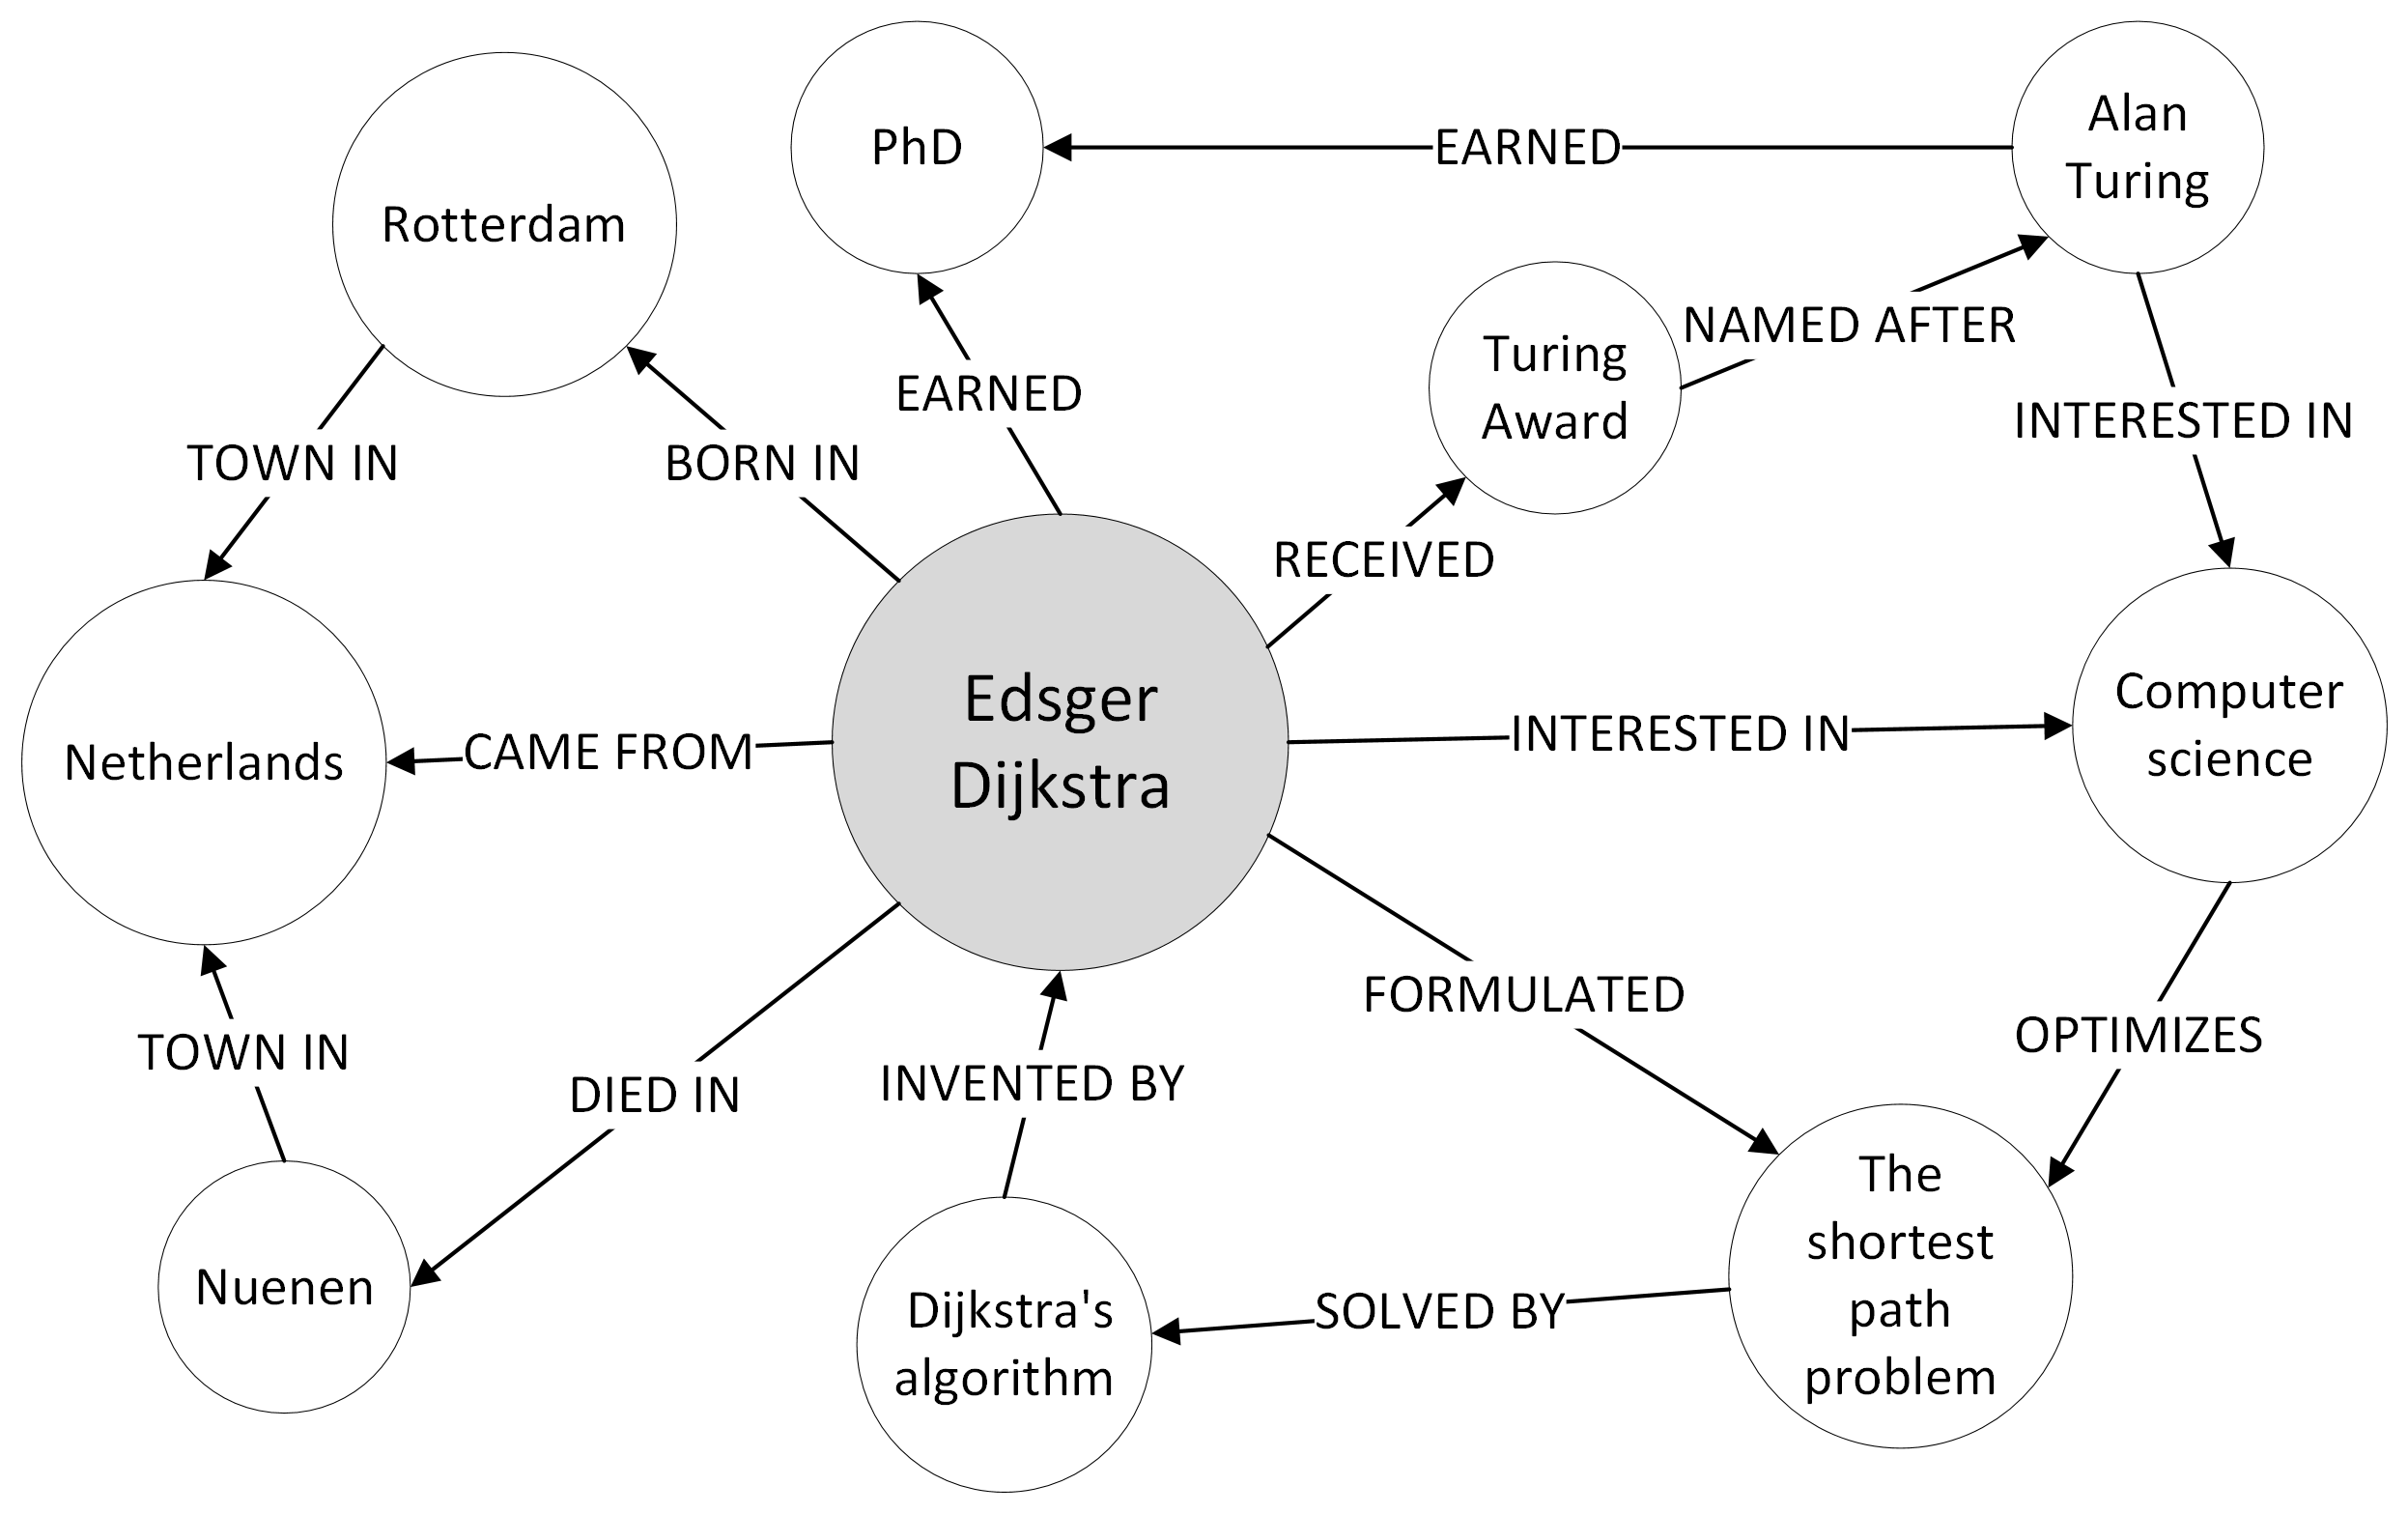
\includegraphics[width=\textwidth]{KnowledgeGraph-Example}
	\caption{Znalostní graf}
	\label{fig:Knowledge-Graph}
\end{figure}

\subsubsection{Hypergrafy}
Tento model obsahuje speciální hrany zvané hyperhrany, které mohou spojovat více vrcholů. Narozdíl od klasické orientované hrany, hyperhrana může mít libovolné množství počátečních a koncových vrcholů. Hypergrafy mohou být užitečné v aplikacích, které zacházejí s vazbami o kardinalitě M:N. Vždy je však možné reprezentovat hypergraf jako LPG. I když s použitím více vztahů a zprostředkujících vrcholů. Příklad hypergrafu je ukázán na obrázku \ref{fig:Hypergraph-Example}.

\begin{figure}[h]
	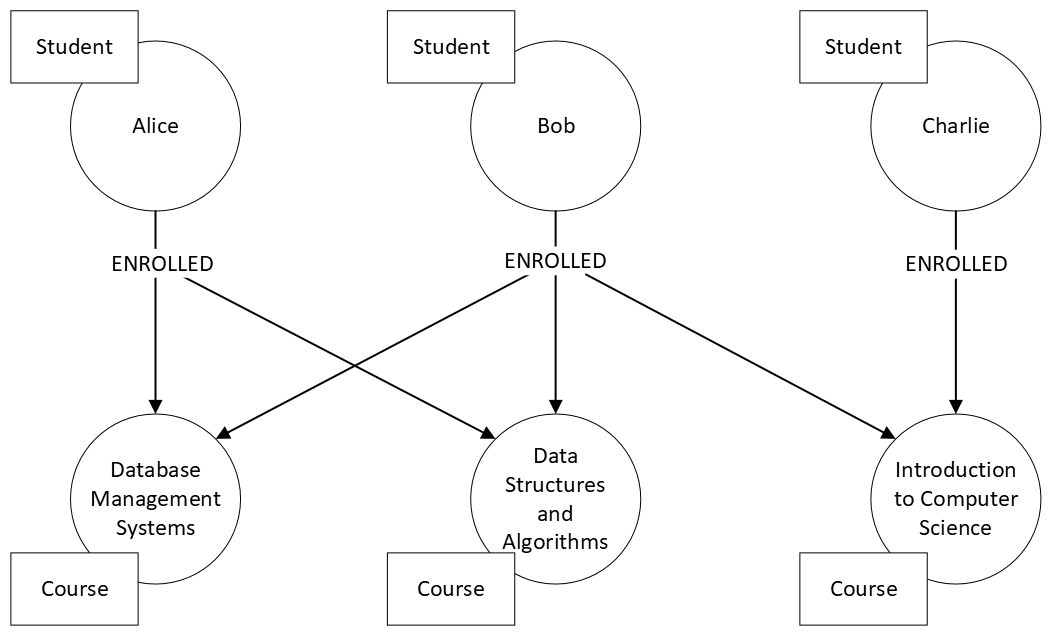
\includegraphics[width=\textwidth]{Hypergraph-Example}
	\caption{Hypergraf}
	\label{fig:Hypergraph-Example}
\end{figure}

\subsection{Systémy OLTP a OLAP}
Při psaní této podkapitoly jsem čerpal též ze zdrojů \cite{oltpOlap} a \cite{cambridge-intelligence}. Grafové databáze dále můžeme rozdělit podle způsobu použití do dvou kategorií:
\begin{itemize}
\item \textit{OLTP systémy}. OLTP je zkratkou za Online Transaction Processing. Jsou navrženy pro rychlé a efektivní zpracování velkého množství transakcí. Nejsou vhodné pro analýzu dat. Dotazy většinou prochází pouze poměrně malý podgraf. Hodí se pro aplikace, ve kterých jsou data v reálném čase čtena, přidávána, mazána a modifikována. Nachází využití například v doporučovacích a bankovních systémech, sociálních sítích a při odhalování podvodů.
\item \textit{OLAP systémy}. OLAP je zkratkou za Online Analytical Processing. Jsou navrženy pro komplexní analýzu velkého objemu dat. Data se z databáze ve většině případů čtou. Zpracovávájí malé množství časově a výpočetně náročných dotazů. Dotazy často operují nad celým grafem. Využívány jsou například v analýze znalostních grafů.
\end{itemize}

\subsection{Výhody grafových databází}
V nativních grafových databázích jsou uloženy nejen entity, ale i vztahy mezi entitami. Při dotazování nedochází k výpočtu těchto vztahů, jak tomu je například u relačních databází pomocí klauzule \texttt{JOIN}. To zrychluje zpracování dotazů pracujících se vztahy mezi entitami. Množství uchovávaných dat obecně výkon nezhoršuje, neboť čas pro vyhodnocení dotazu závisí pouze na velikosti podgrafu, kterým procházíme.

Pomocí vrcholů a hran lze často lépe vystihnout dané problémy, než například pomocí tabulek. Grafová struktura popisuje, jak nad daty v rámci aplikace přemýšlíme. Lze tak dosáhnout datových modelů, které jsou srozumitelné i laikům. Navíc ve spoustě případů je dotazování prostřednictvím grafových dotazovacích jazyků přehlednější než dotazy v jiných databázích. To platí především pro dotazy pracující se vztahy mezi entitami.

Většina grafových databází nevynucují definování schématu. Tato vlastnost databází se označuje \textit{schema-less}. Struktura dat se může měnit v závislosti na~potřebách aplikace. Přidávání nových vlastností, vrcholů, hran a labelů nenarušuje chod aplikace. To přináší jisté výhody pro vývojáře a budoucí vývoj. Ovšem základní forma dat by měla být známa, abychom mohli s daty pracovat.

Některé grafové databáze (hlavně OLAP systémy) nabízí grafové algoritmy, které lze aplikovat na~uložená data. To rozšiřuje možnosti analýzy propojených dat, které by jinak byly obtížně realizovatelné.

I přes komplikované rozdělení grafových dat (sharding) mnoho implementací grafových databází nabízí \textit{horizontální škálování}. To umožňuje rozdělit data mezi více výpočetních strojů. Je spousta technik jak data rozdělit. Například pomocí hashování identifikátorů, nebo pomocí grafových vzorů. Ale volba správné techniky je obtížná. Pro co největší efektivitu databáze by měl být celý graf rozdělen na podgrafy tak, aby mezi jednotlivými podgafy bylo co nejméně hran, které by je propojovaly. Tyto podgrafy budou uloženy na jednotlivých strojích.\cite{practitioner}

\subsection{Nevýhody grafových databází}
Grafové databáze jsou mezi ostatními druhy databází relativně mladé. Narozdíl od relačních databází, kde většina z nich alespoň z části implementují SQL (zkratka pro Structured Query Language), je všechny mezi sebou nepropojuje jeden standardizovaný dotazovací jazyk. Jeho absence škodí jejich popularitě, neboť pro vývojáře znamená, že pro práci s více grafovými databázemi je nucen používat více různých dotazovacích jazyků, místo specializování se na jeden univerzální. Navíc při změně grafové databáze hrozí, že bude nutné přepsat všechny dotazy do jiného dotazovacího jazyka. Několik grafových databází proto vyžívají pro dotazování speciálně upravený jazyk SQL. Jednou z nich je OrientDB. Tento problém by se však mohl v blízké době zlepšit. Podle zdroje \cite{GQL} se pracuje na~normovaném jazyku GQL, což je zkratka pro Graph Query Language.

Grafovým databázím dělají problém dotazy, které operují nad celým grafem. Jedná se především o filtrování a agregování. Pokud se v aplikaci soustředíme především na takové typy operací, je lepší zvolit jiné databázové technologie.

Jelikož jsou grafové databáze často schema-less, tak může docházet k nekonzistenci ukládaných dat. Ne všechny implementace grafových databází totiž disponují mechanismy, které by v případě potřeby nekonzistenci zabránily. Konzistence dat je tedy v některých databázích řešena pouze na aplikační úrovni.

\subsection{Implementace grafových databází}
Existuje spousta implementací grafových databází. Liší se například nativností, dotazovacím jazykem, škálovatelností a podporou ACID transakcí. ACID je zkratkou pro čtyři žádané vlastnosti databázových transakcí: atomicita, konzistence, izolovanost a trvalost. Jakou z nich využít pro naši aplikaci je otázka zkoumání funkcionalit jednotlivých implementací. Známými grafovými databázemi jsou například:

\begin{itemize}
\item \textit{Amazon Neptune} -- rychlý, spolehlivý, plně řízený a vysoce zabezpečený systém pro hustě propojené grafy. Podporuje jak LPG, tak RDF grafový model. Databáze byla představena v roce 2017 společností Amazon. Výhodou je podpora známých dotazovací jazyků Gremlin, openCypher a SPARQL.\cite{amazonNeptune}
\item \textit{TigerGraph} -- moderní, nativní grafová databáze pro ukládání LPG grafových modelů. Nabízí vestavěné paralelní výpočty nad grafy.\cite{tigerGraph}
\item \textit{AllegroGraph} -- výkonná multi-model open-source databáze. Data mohou být ukládána ve formě RDF grafu, vektorů nebo dokumentů. AllegroGraph je kompatibilní se standardy W3C/ISO a podporuje dotazy prostřednictvím SPARQL a Prologu.\cite{allegroGraph} Dle knihy \cite{graphDatabases} nemá nativní grafové zpracování.
\item \textit{JanusGraph} -- jedná se o open-source projekt společnosti The Linux Foundation. Jedná se o odnož grafové databáze Titan. Je založen na Apache TinkerPop, a proto lze klást dotazy prostřednictvím jazyka Gremlin. Kromě online transakčního zpracování (OLTP) podporuje JanusGraph globální grafovou analýzu (OLAP) díky integraci Apache Spark.\cite{janusGraph}
\end{itemize}
V rámci práce byly zkoumány tři implementace grafových databází: \textit{Neo4j}, \textit{OrientDB} a \textit{ArangoDB}.

\subsubsection{Neo4j}
Při psaní této podkapitoly jsem čerpal též ze zdrojů \cite{neo4jDoc} a \cite{neo4jDev}. Databázový systém Neo4j je nejrozšířenější open-source grafovou databází na trhu s největší uživatelskou základnou. Nabízí vysoký výkon při práci s grafy. Její první verze byla vyvinuta v roce 2002. Vznikla z důvodu nespokojenosti jejich zakladatelů s výkonem relačních databází. Implementována je v Javě. Jedná se o nativní schema-less grafovou databázi. Je využívána světoznámými společnostmi jako jsou Microsoft, eBay, nebo Linkedin. Klást dotazy můžeme prostřednictvím dotazovacího jazyka Cypher, který byl navržen přímo vývojáři Neo4j. Dotazy se nejběžněji píší a vyhodnocují v rozhraní nazvaném Neo4j Browser. Výsledky dotazů umožňuje zobrazit v grafové podobě, tabulce, nebo třeba JSON formátu. Při lokálním použití je Neo4j Browser dostupný na adrese \url{http://localhost:7474/browser}.

Neo4j používá pro vrcholy a hrany identifikátory s názvem \textit{elementId}. Dle dokumentace však není bezpečné používat tyto identifikátory v jednotlivých transakcích a je doporučeno, pokud je jich potřeba, si vytvořit vlastní. Pro rychlý přístup k datům mají záznamy v databázi fixní délku. V úložišti jeden vrchol zabírá 15~bytů a jedna hrana 34 bytů. Na disku jsou ukládány ve spojových seznamech. Vlastnosti jsou ukládány odděleně, jsou propojeny s vrcholy a hranami pomocí pointeru a jsou čteny jen v případě potřeby.

Neo4j lze provozovat jako samostatně spravovanou databázi, nebo jako cloudovou databázi. Pro první případ existují dvě varianty – Community Edition a Enterprise Edition. Community Edition je open source. Enterprise Edition se dále liší mimo jiné lepším zabezpečení, zálohováním, škálováním, podporou běhu více databází na~jednom stroji a monitorováním databáze. Pro cloudové nasazení nabízí Neo4j plně automatizovaný databázový servis s názvem Neo4j AuraDB, spuštěný v roce 2019. AuraDB je dostupný i v bezplatné verzi, která je však omezena na~200~tisíc vrcholů a 400 tisíc hran.

Neo4j má též spoustu rozšiřujících knihoven a nástrojů, které lze do produktů doinstalovat (pokud již nejsou součástí). Například se jedná o nástroj pomáhající při migrování dat z relační databáze do Neo4j, nebo o standardní knihovnu procedur a funkcí. V práci je pak ukázána knihovna s užitečnými grafovými algoritmy.

\subsubsection{OrientDB}
Při psaní této podkapitoly jsem čerpal též ze zdrojů \cite{orientDBDoc} a \cite{benchmark}. OrientDB je open-source NoSQL databázový systém implementovaný v Javě. Byl představen v roce 2010 (komerčně 2011). Jedná se o pokročilou multi-model databázi. Podporuje grafový, dokumentový, klíč-hodnota a objektový model. Databáze je schématicky flexibilní. Umožňuje uchovávat schema-full, schema-less a schema-hybrid data. Manipulovat s databází můžeme pomocí programovacího jazyka Java, speciálně upraveného SQL a dotazovacího jazyka Gremlin.

Uživatelé pak mohou interagovat s databází pomocí Java API, HTTP REST API, konzolu nebo prostřednictvím grafického uživatelského rozhraní nazvaného OrientDB Studio. Pokud databázový server běží lokálně, OrientDB Studio lze otevřít ve webovém prohlížeči na adrese \url{http://localhost:2480}. V~něm lze mimo jiné spravovat jednotlivé databáze, práva uživatelů, klást SQL dotazy a zobrazovat výsledky v mnoha formátech.

Nejmenší jednotkou v databázi je \textit{záznam} (record). Rozlišujeme 4 typy záznamů: Documents, Blobs, Vertices a Edges. Tyto záznamy jsou organizovány do \textit{tříd} podobně, jako je tomu v objektově orientovaném programování. Každý záznam pak patří právě do jedné třídy. Třídy mohou dědit z jiných tříd. Pro vrcholy je výchozí třídou \texttt{V}, pro hrany pak třída \texttt{E}. Je silně doporučené vytvářet vlastní definované třídy pro vrcholy a hrany dědící právě z těchto tříd. Každá třída má dále přidělené vlastní \textit{klastry}. Ty představují fyzický prostor, kam OrientDB ukládá záznamy. Vytvoří se automaticky spolu se třídou. Název klastru je pak odvozen z názvu třídy. Pro zlepšení výkonu je vytvořeno tolik klastrů, kolik má CPU na serveru jader. Každému záznamu v databázi je na základě jeho pozice v klastru automaticky vygenerován unikátní identifikátor, označovaný jako RID, což je zkratka pro Record ID. RID je uchováván ve~formátu \textit{\#<klastrId>:<pozice>}.

OrientDB též umožňuje takzvané \textit{lightweight} hrany, které zlepšují výkon a~snižují nároky na úložiště. Tyto hrany však nemohou mít žádné vlastnosti, neboť jsou v databázi reprezentovány pomocí přímých referencí mezi vrcholy.

V práci je využívána bezplatná verze OrientDB Community Edition. OrientDB nabízí i placenou verzi Enterprise Edition, která poskytuje výhody jako správu zálohování, migrační nástroje, monitorování systému a CRUD operací v~reálném čase a jiné.

\subsubsection{ArangoDB}
Při psaní této podkapitoly jsem čerpal též ze zdroje \cite{arangoDBDoc}. ArangoDB je multi-model open-source databáze. Lze ji použít jako plnohodnotné úložiště dokumentů, grafů, párů klíč-hodnota, full-text vyhledávací engine nebo jakoukoli kombinaci těchto technologií. První verze byla představena společností ArangoDB Inc. v roce 2012. S daty je možno pracovat prostřednictvím jazyka AQL (ArangoDB Query Language). Pokud server provozující ArangoDB běží lokálně je možno interagovat s databází skrze webové rozhraní na adrese \url{127.0.0.1:8529}, nebo prostřednictvím textového rozhraní \textit{arangosh}. Lze též komunikovat prostřednictvím HTTP API, nebo driveru. Ačkoli je ArangoDB schema-less, umožňuje vynutit strukturu dokumentů v rámci kolekcí. Toho lze dosáhnout pomocí definování \textit{JSON Schema}\footnote{\url{https://json-schema.org/}} formátu. Databáze nabízí též placenou verzi, nabízející například vyšší výkonnost, zabezpečení a škálování grafů.

Data jsou ukládána ve formátu JSON. Nejmenší jednotkou v databázi je \textit{dokument}, který představuje jeden záznam dat. Dokumenty jsou ukládány v binární podobě zvané \textit{VelocyPack}. Dokumenty jsou dále organizovány do \textit{kolekcí}, které mohou obsahovat libovolné množství dokumentů. Každý dokument patří právě do jedné kolekce. Každý dokument má dále \textit{atributy}, které slouží jako vlastnosti. Každý dokument navíc obsahuje minimálně 3 povinné atributy, nazývané \textit{systémové}. Jsou odlišeny od ostatních tak, že začínají podtržítkem. Mají datový typ \texttt{string} a všechny jsou určené pouze ke čtení.
\begin{itemize}
\item \textit{\_key} -- nazývá se \textit{dokumentový klíč}. Každý dokument v rámci kolekce má hodnotu tohoto atributu unikátní. Dokumentový klíč lze specifikovat při vytváření dokumentu. Pak jej již nelze změnit. Pokud není specifikován, je atributu přiřazena hodnota automaticky.
\item \textit{\_id} -- nazývá se \textit{dokumentový identifikátor}. Každý dokument v rámci databáze má hodnotu tohoto atributu unikátní. Je uchováván ve formátu \textit{<název-kolekce>/<klíč-dokumentu>}.
\item \textit{\_rev} -- nazývá se \textit{dokumentová revize}. Hodnota atributu je automaticky obdržena serverem.
\end{itemize}
Hrany v databázi jsou uloženy ve speciálních dokumentech a kolekcích nazvané \textit{hranové}. A mají navíc dva systémové atributy.
\begin{itemize}
\item \textit{\_from} -- hodnota atributu je rovna dokumentovému identifikátoru počátečního vrcholu.
\item \textit{\_to} -- hodnota atributu je rovna dokumentovému identifikátoru koncového vrcholu.
\end{itemize}

Databáze nepoužívá přímo index-free adjacency. Místo toho používá tzv. hybridní index. Jeho výhoda se dle ArangoDB projeví u větších grafů, které celé nejdou načíst do paměti. Hybridní index kombinuje výhody spojového seznamu a hashovací tabulky, přičemž dosahuje časové složitosti $O(k)$ v případě procházení grafu, kde $k$ je stupeň vrcholu, a $O(1)$ při editování a mazání hran. Oproti tomu index-free adjacency má i v případě mazání a editování v nejhorším případě časovou složitost $O(k)$, což se negativně projevuje převážně u superuzlů. \cite{hybridIndex}

\subsection{Dotazovací jazyky v grafových databázích}
Pomocí dotazovacích jazyků lze formulovat dotazy, které lze klást na databázi. Pomocí nich lze definovat \textit{grafové vzory}. Ty popisují, jakým způsobem grafem procházíme. Na základě specifikovaných vzorů a mechanismu zvaném pattern matching následně můžeme dostat odpovědi na dotazy.

Jak již bylo zmíněno pro grafové databáze zatím neexistuje jeden standardní jazyk. Lze narazit na jazyky vyvinuté specificky pro konkrétní systém. Příkladem může být jazyk \textit{Cypher} vyvíjený společností Neo4j nebo \textit{AQL} využívaný v databázi ArangoDB. Na druhou stranu jsou zde jazyky, jakým je například \textit{Gremlin}, které lze použít ve více systémech zacházejících s grafy -- například v~OrientDB. Následující seznam obsahuje další známé dotazovací jazyky.
\begin{itemize}
\item \textit{SPARQL} -- je standardizovaný dotazovací jazyk využívaný v grafových databázích implementujících RDF model. \cite{sparql}
\item \textit{PGQL} -- je jednou z komponent datové databáze společnosti Oracle, který je rozšířením SQL. Podporuje jak LPG, tak RDF grafový model. Implementuje vestavěné grafové algoritmy.\cite{pgql}
\item \textit{GSQL} -- je procedurální jazyk používaný v databázi TigerGraph podobný SQL. Slibuje vysoký výkon díky vestavěnému paralelismu.\cite{gsql}
\item \textit{GraphQL} -- jedná se o dotazovací jazyk pro API, který není závislý na~konkrétní implementaci. Za jeho vývojem stojí Facebook. Je povážován za~přímého konkurenta REST API.\cite{graphql}
\end{itemize}

\subsubsection{Cypher}
Při psaní této podkapitoly jsem čerpal též ze zdrojů \cite{neo4jDoc} a \cite{neo4jDev}. Cypher je inspirovaný známým jazykem SQL z relačních databází. Důkazem může být použití několika stejnojmenných klíčových slov, jako je \texttt{WHERE}, \texttt{LIMIT}, \texttt{ORDER BY} apod. V obou případech se jedná o deklarativní dotazovací jazyky.

Cypher je unikátní při definování grafových vzorů, kde využívá kulaté závorky pro vrcholy a hranaté pro hrany, čímž docílí lepší přehlednosti v dotazu. Základní syntaxe pro průchod grafem z vrcholu \textit{vrchol1} na vrchol \textit{vrchol2}, přes hranu \textit{HRANA}, která je spojuje, je ve formátu 

\begin{center}
\textit{(vrchol1)-[:HRANA]->(vrchol2)}.
\end{center}

%https://neo4j.com/docs/cypher-manual/current/planning-and-tuning/execution-plans/#lazy-eager-evaluation
Pro úsporu paměti implementuje vždy, když je to možné, \textit{líné vyhodnocování dotazů}. Tedy u většiny operátorů nečekáme na všechny výsledky aplikace daného operátoru, ale hned po jejich získání na ně aplikujeme další nadřazený operátor. Výpočet podřazeného operátoru tedy obecně nemusí skončit dříve, než na výsledky začneme aplikovat nadřazený operátor. Tím nedochází k zatěžování paměti mezivýsledky výpočtu. Nicméně ne všechny dotazy lze takto vyhodnocovat. Pro operace jako je třídění nebo agregování je nutné použít \textit{striktní vyhodnocování dotazů}. S výsledky pak nadřazený operátor manipuluje až po úplném skončení výpočtu.

\subsubsection{Gremlin}
Při psaní této podkapitoly jsem čerpal též ze zdrojů \cite{practicalGremlin}, \cite{tinkerPopDoc} a \cite{orientDBDoc}. Gremlin je dotazovací jazyk pro procházení grafů, který je součástí grafového výpočetního frameworku Apache TinkerPop\footnote{\url{http://tinkerpop.apache.org/}}. Gremlin lze použít pro všchna grafová úložiště, která tento framework podporují. Je to imperativní jazyk s nějakými deklarativními prvky. Podobně jako Cypher ve většině případů vyhodnocuje dotazy líným způsobem.

Apache TinkerPop mimo jiné obsahuje také Gremlin Console, což je textové REPL (Read-Eval-Print Loop) rozhraní pro práci s lokálními, či vzdálenými grafy. Je založená na Groovy konzoli. Groovy je programovací jazyk, který je označován jako nadmnožina Javy. Co funguje v Javě funguje i v Groovy. V~konzoli tedy můžeme používat validní kód napsaný v tomto jazyce. Díky tomu lze například uložit do proměnné určitý vrchol a na něj se pak přes danou proměnnou odkazovat. Konzole je široce rozšiřitelná pomocí různých pluginů.

Pro napojení konzole na databázi OrientDB budeme potřebovat plugin\linebreak \texttt{tinkerpop.orientdb}. Když je tento plugin aktivovaný, lze v konzoli vytvořit novou instanci \texttt{OrientGraph}. Uložíme ji do proměnné \texttt{graph}. Při vytváření je nutné specifikovat URL pro připojení k databázi. Připojit se můžeme k lokální databázi, vzdáleně k databázovému serveru nebo k jednorázové databázi v paměti. Může být též potřeba zadat přihlašovací údaje. Než začneme psát dotazy pomocí Gremlinu musíme ještě vytvořit instanci zdrojového objektu pro procházení grafu zavoláním metody \texttt{traversal()} na hodnotu v proměnné \texttt{graph}. Ta se ukládá ve většině případů do proměnné \texttt{g}. Celý postup je uveden ve zdrojovém kódu \ref{kod:establishConnection}.

\begin{listing}[h]
\begin{minted}{Groovy}
//OrientDb database connector
graph = OrientGraph.open(url, user, password);

//establishing a graph traversal source object
g = graph.traversal();
\end{minted}
\caption{Připojení se k databázi OrientDB v Gremlin Console.}
\label{kod:establishConnection}
\end{listing}

\subsubsection{AQL}
Při psaní této podkapitoly jsem čerpal též ze zdroje \cite{arangoDBDoc}. Jedná se o~převážně deklarativní dotazovací jazyk používaný v databázi ArangoDB. Snaží se být nezávislý na klientovi. To znamená, že jazyk a syntaxe není závislá na programovacím jazyku, který klient využívá. Obdobně jako velká čast grafových dotazovacích jazyků je ovlivněný jazykem SQL. Jazyk je jednotný pro všechny databázové modely. AQL je čistě DML (zkratka pro Data Manipulation Language) jazyk. Tedy umí číst a manipulovat s daty v kolekcích. Neumí vytvářet a odstraňovat databáze, kolekce a indexy.

Každý dotaz v AQL musí buď vracet výsledky pomocí klíčového slova\linebreak \texttt{RETURN}, nebo provádět operaci, která modifikuje data. Je podporován pouze jeden dotaz v rámci jednoho dotazovacího řetězce. Není možné provést výpočet více oddělených dotazů pro jedno zavolání. Dotaz je opět vyhodnocován líně, pokud se v něm neobjevují poddotazy, ty jsou ve výrazech vyhodnocovány předem. Příkladem je ternární operátor. Dotazy lze klást prostřednictvím webového rozhraní nebo konzole \textit{arangosh}. V práci se dotazy kladly pouze prostřednictvím první zmíněné možnosti.
\clearpage
\section{Modelování grafových dat}
Tato kapitola byla napsána s využitím knih \cite{inAction}, \cite{graphDatabases}, \cite{practitioner}. Dále byly využity tyto zdroje \cite{ionos} a \cite{neo4jDev}.

Při \textit{modelování grafových dat} se snažíme navrhnout grafový model, který bude reprezentovat náš problém. Jedná se o proces, ve kterém rozpoznáváme jednotlivé entity, které v problému vystupují a vztahy mezi nimi. Problém pak popisujeme jako graf skládající se z vrcholů a hran pomocí vlastností a labelů. Podoba výsledného modelu závisí na potřebách vyvíjené aplikace a otázkách, které mají podobu dotazů, které budou na databázi kladeny.

Dodržení základních principů modelování dat je důležité pro výslednou efektivitu. Pro správné fungování je proto dobré věnovat grafovému modelování dostatečné množství času. Když je graf přizpůsoben dotazům, dokáže velmi rychle nalézt potřebnou odpověď. Naopak špatně zvolený model grafu může ve výsledku aplikaci ublížit a být překážkou. Například tím, že zpracování dotazu bude trvat déle než u optimalizovaného modelu.

Další důležitou věcí, na kterou je potřeba myslet, je budoucnost vyvíjené aplikace. Model by měl být připravený na možné změny, které po aplikaci budou její koncoví uživatelé požadovat.

Je potřeba také podotknout, že ne všechna data jsou vhodná pro uchovávání v grafové podobě. Rozhodnutí, zda pro naše účely je grafová databáze dobrým řešením, je ve spoustě případů náročné. Existují různé typy databází a každá má své silné a slabé stránky. Grafové databáze jsou výhodné pro aplikace, které mají vztahy mezi entitami na prvním místě. Tato vlastnost by měla být odrazovým můstkem při rozhodování, zda použít, či nepoužít grafovou databázi. Lze dohledat spoustu \uv{návodů} pomáhajících s touto volbou. Jeden z nich je ukázán na obrázku \ref{fig:GraphDatabase-DecisionTree}. Je na něm zobrazen rozhodovací strom převzatý z knihy \cite{inAction}.

\begin{figure}
	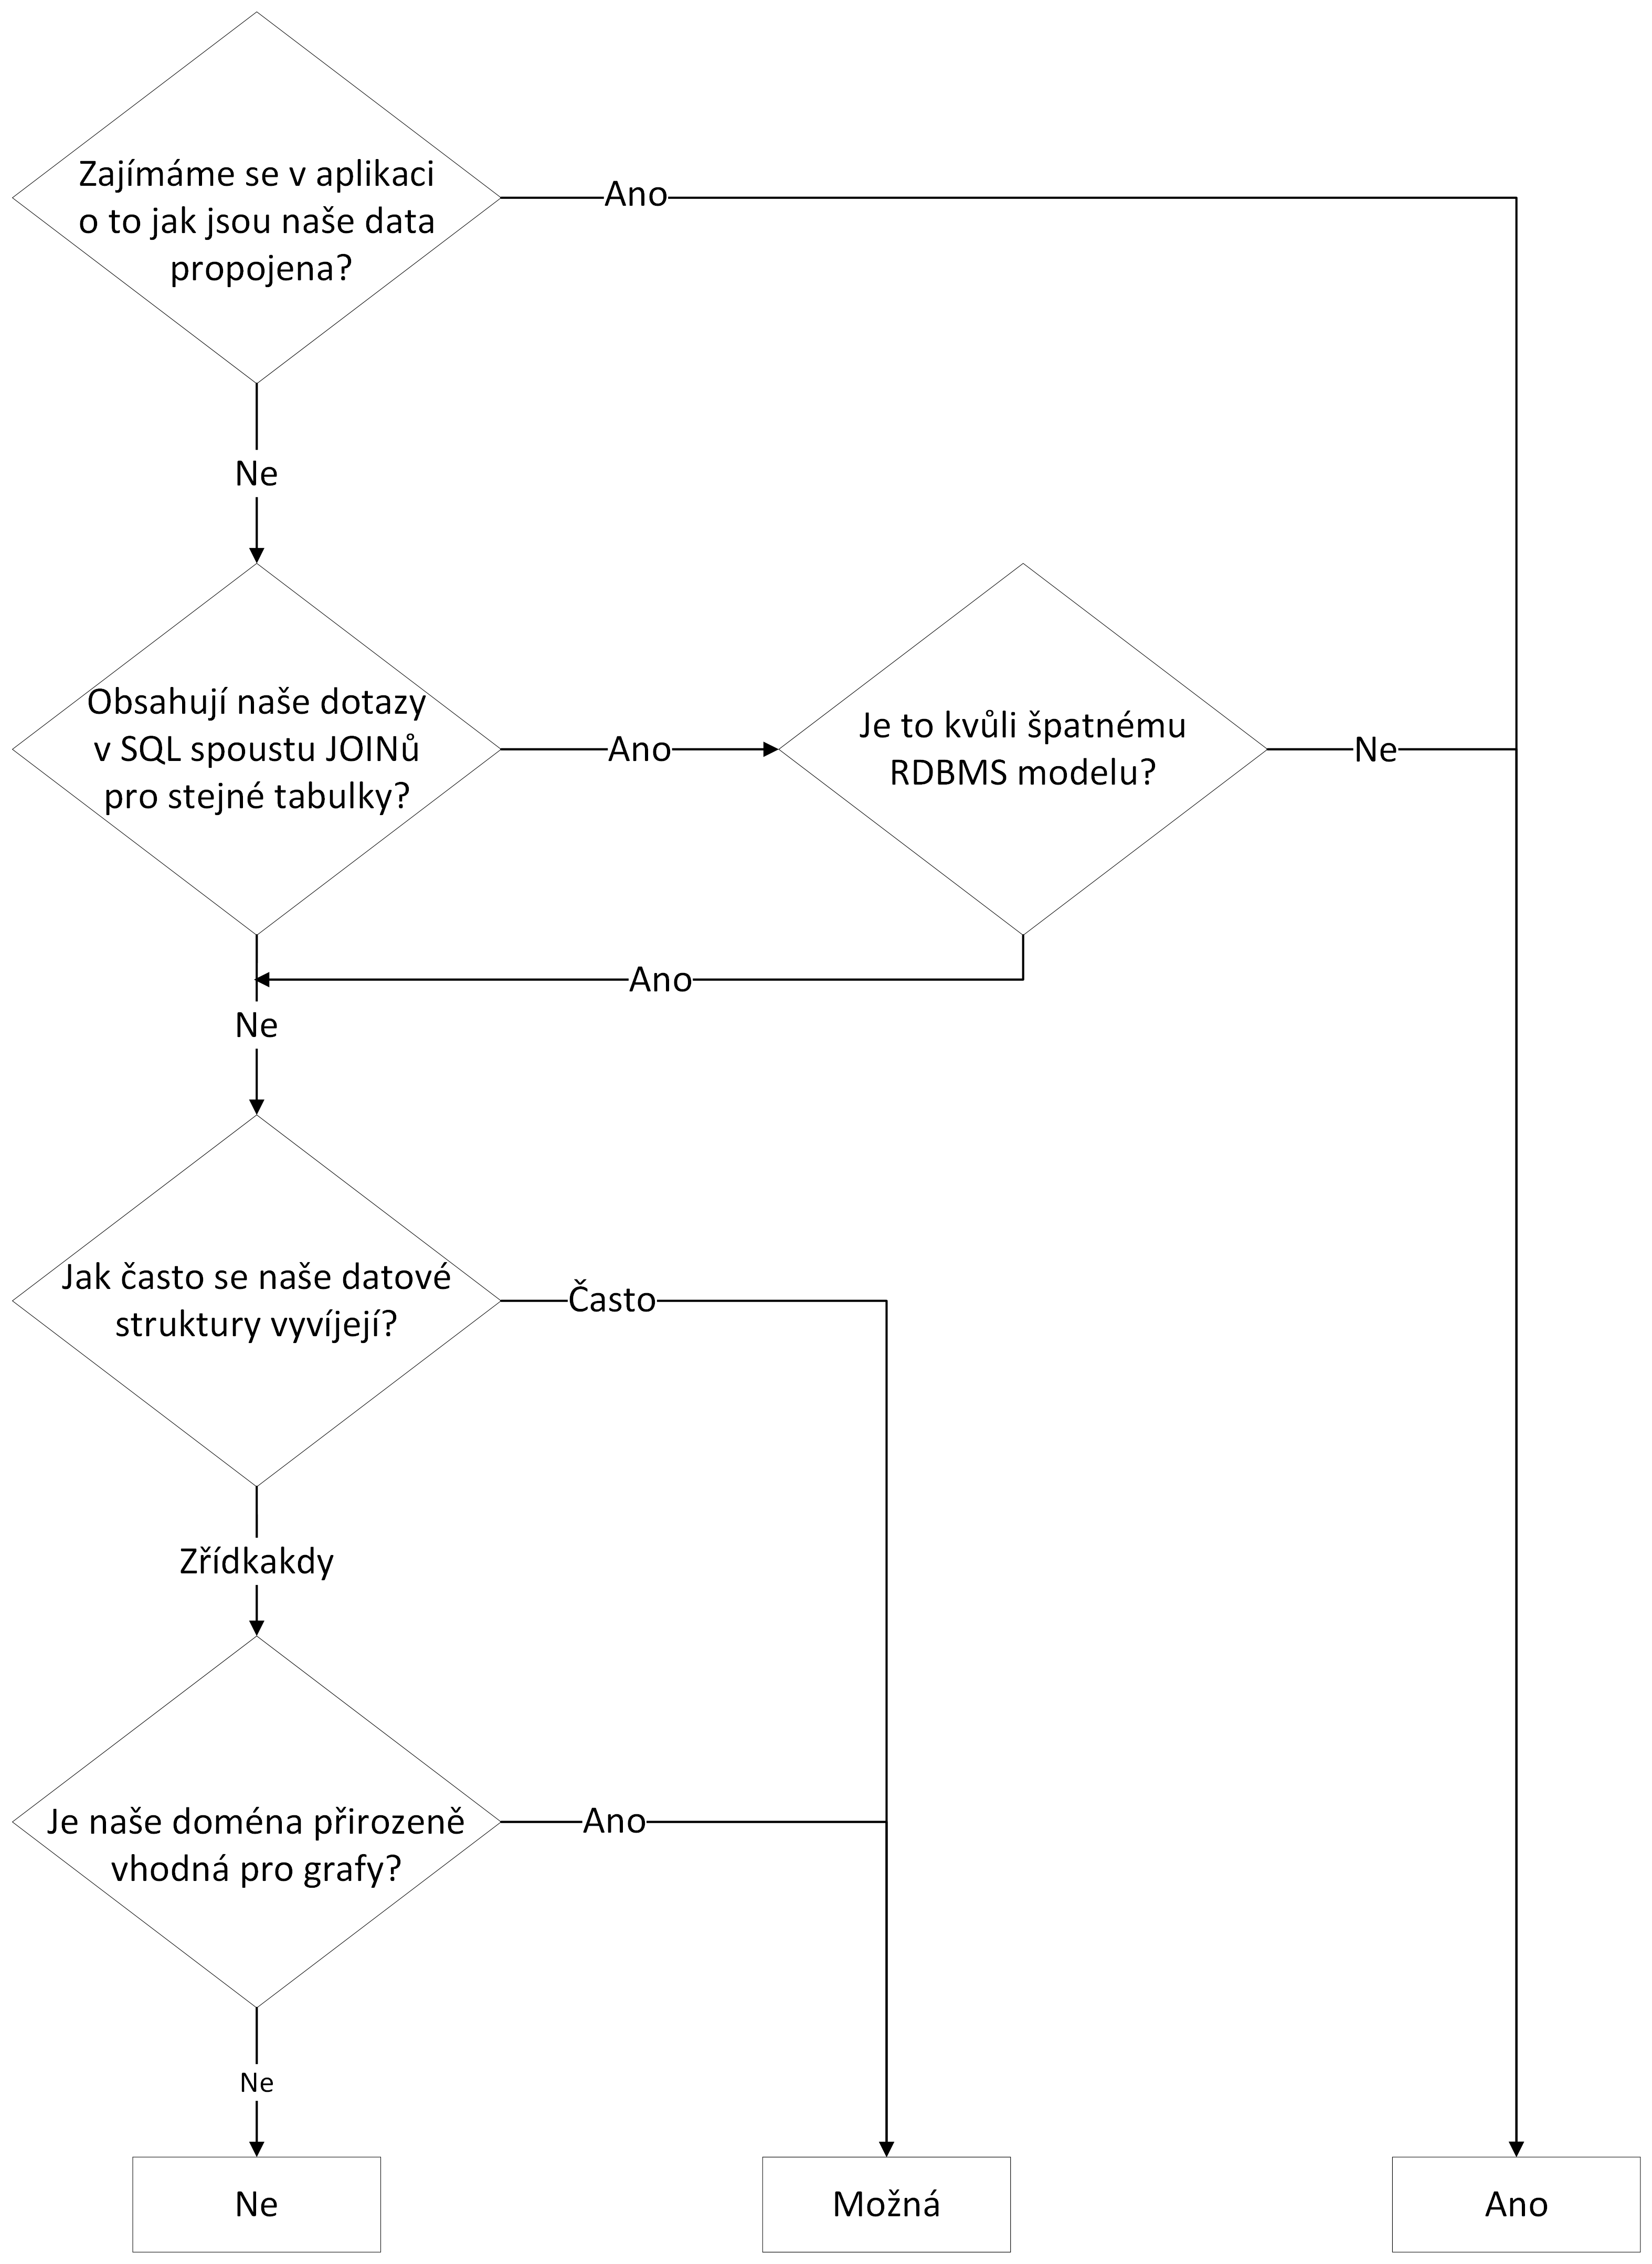
\includegraphics[width=\textwidth]{GraphDatabase-DecisionTree}
	\caption[Rozhodovací strom.]{Rozhodovací strom pro vhodnost použití grafové databáze.}
	\label{fig:GraphDatabase-DecisionTree}
\end{figure}

Pokud se pro použití grafové databáze rozhodneme, můžeme přistoupit k modelování dat. V této kapitole se na návrh grafového modelu zaměříme. Zkusíme si to na příkladu sociální platformy pro nadšence cestování. Sociální sítě jsou totiž jedním z případů, kdy použití grafových databází pro ukládání dat dává smysl. Tato aplikace tedy bude umožňovat cestovatelům se propojit s ostatními. Dále bude zaznamenávat jejich výlety do různých destinací, hodnocení těchto cest, cestovatelské aktivity, které destinace nabízí a které se mohou uživatelům aplikace líbit. Na základě přátel a hodnocení cest do destinací aplikace dokáže uživateli doporučit jiné destinace, které dosud nenavštívil. Naše aplikace se tedy bude dotýkat i dalšího případu užití grafových databází, a to systémů pro doporučování, které jsou v praxi hojně využívány.

Výsledný model je též dostupný v elektronické příloze práce, kde jsou pro jeho vyzkoušení předpřipravené dotazy a csv soubory obsahující data pro naši aplikaci. Seznam všech csv souborů, rozdělený na entity a vztahy mezi nimi a~počet řádků jednotlivých souborů lze vyčíst z tabulky \ref{tab:TravelEnthusiastNetwork-csv}.

\begin{table}[h]
\caption{Použité soubory v aplikaci pro cestovní nadšence.}
\label{tab:TravelEnthusiastNetwork-csv}
\begin{tabularx}{\textwidth}{ | l | c | c | X | }
 \hline
 \textbf{Typ} & \textbf{Název souboru} & \textbf{Počet} & \textbf{Informace o souboru} \\
 \hline \hline
 \multirow{6}{*}{Entity} & \texttt{activities.csv} & 48 & Cestovatelské aktivity, které mohou destinace nabízet. \\
 & \texttt{countries.csv} & 57 & Státy, v kterých se vyskytují jednotlivé destinace.\\
 & \texttt{destinations.csv} & 203 & Destinace, které mohou uživatelé navštívit. \\
 & \texttt{journeys.csv} & 296 & Cesty, v rámci kterých uživatelé navštěvují destinace. \\
 & \texttt{ratings.csv} & 640 & Hodnocení jednotlivých cest uživateli.\\
 & \texttt{users.csv} & 300 & Uživatelé sociální sítě Travel Enthusiast Network.\\
 \hline
 \multirow{8}{*}{Vztahy} & \texttt{follows.csv} & 6091 & Uživatel sleduje uživatele. \\
 & \texttt{is\_within.csv} & 203 & Destinace je ve státu. \\
 & \texttt{led\_to.csv} & 1496 & Cesta vedla do destinace.\\
 & \texttt{likes.csv} & 1460 & Uživatel má rád cestovní aktivitu. \\
 & \texttt{offers.csv} & 2028 & Destinace nabízí cestovní aktivitu.\\
 & \texttt{participated.csv} & 1643 & Uživatel se zúčastnil cesty. \\
 & \texttt{wrote\_about.csv} & 640 + 640 & Uživatel napsal recenzi o cestě. \\
 \hline
\end{tabularx}
\end{table}
\pagebreak
Postup modelování se dá dle \cite{inAction} rozdělit do čtyř fází:
\begin{enumerate}
  \item Definice problému,
  \item konceptuální datový model,
  \item logický datový model a
  \item testování modelu.
\end{enumerate}
V následujících částech se na jednotlivé fáze podíváme detailněji. 

\subsection{Definice problému}
\label{sec:problem-definition}
V první fázi bychom měli zvážit, co všechno by měla aplikace umět. Výsledkem by měl být její, co nejpřesnější, slovní popis. Pomoci nám může odpovědět na~pár otázek převzatých z knihy \citep{inAction}.

\subsubsection{Co od aplikace očekáváme?}
Aplikace je sociální sítí, a proto by měla jednotlivým uživatelům umožňovat se propojit s ostaními uživateli aplikace. To je umožněno pomocí relace sledování. Uživatelům by pak na základě jimi sledovaných uživatelů, oblíbených aktivit a~hodnocení destinací měly přicházet tipy na výlet. Aplikace by měla umožnit zazanamenat, že někteří uživatelé podnikli cestu společně. Uživatelé budou moci v~rámci jedné cesty navštívit více destinací. Tyto podniknuté cesty mohou uživatelé ohodnotit.

\subsubsection{Jaké informace budou v databázi uchovávány?}
\begin{itemize}
  \item Potřebné údaje o uživatelích -- jejich jméno, příjmení, unikátní identifikátor, oblíbené cestovatelské aktivity.
  \item Informace o cestách, které uživatelé podnikli -- název cesty, časové údaje, jejich recenze.
  \item Informace o destinacích -- lokace, název, nabízené cestovatelské aktivity.
\end{itemize}
V reálném scénáři by projekt pravděpodobně zahrnoval mnoho dalších informací, ale pro tuto ukázkovou aplikaci to ponecháme omezené. Pro zjednodušení se vyhneme přesným souřadnicovým informacím a vystačíme si s informací v rámci jakého státu se daná destinace nachází. Dále uživatelům aplikace bude dovolovat psát hodnocení pouze na dané cesty, nikoli na destinace, které v rámci cesty podnikli. Uživatelé mohou hodnotit pomocí přirozených čísel na stupnici od 1 do 5, přičemž číslo 5 představuje nejvyšší hodnocení. Uživatelé cestující spolu se budou účastnit stejné cesty do destinací.

\subsubsection{Jak spolu tyto informace vzájemně souvisí?}
Následující seznam ukazuje, jakým způsobem jsou odpovědi na předchozí otázku mezi sebou propojeny. 
\begin{itemize}
  \item Uživatel \textbf{sleduje} jiného uživatele.
  \item Uživatel \textbf{se zúčastnil} cesty \textbf{vedoucí do} destinace.
  \item Uživateli se \textbf{líbí} cestovatelská aktivita.
  \item Uživatel \textbf{napsal} recenzi \textbf{o} cestě.
  \item Destinace \textbf{nabízí} cestovatelskou aktivitu.
  \item Destinace \textbf{je ve} státě.
\end{itemize}

\subsubsection{Na jaké otázky potřebujeme v aplikaci najít odpověď?}
\begin{itemize}
  \item Jaké všechny uživatele sleduji? A koho sledují oni? Které uživatele nesleduji, ale sledují je uživatelé, které sleduji?
  \item Najdi 3 nejlépe hodnocené destinace, které jsem nenavštívil, nabízející konkrétní cestovní aktivity.
  \item Které destinace navštívil uživatel X? Kolikrát je navštívil?
  \item S kterými uživateli podnikl cestu uživatel X?
  \item Najdi destinace nabízející některé z cestovatelských aktivit, které se uživateli líbí. Seřaď je na základě hodnocení.
  \item Pro konkrétní destinaci vrať 3 měsíce v roce, ve kterých je nejlépe hodnocená.
  \item Najdi uživatele, jejichž jméno nebo přijmení obsahuje řetězec XYZ. 
\end{itemize}
Tyto otázky po vytvoření modelu přeložíme pomocí dotazovacího jazyka na dotazy.
 
\subsection{Konceptuální datový model}
V této fázi vyvineme konceptuální datový model, což je přehledný diagram popisující typy dat a jejich propojenost v naší aplikaci. Vyvarujeme se v něm pro nevývojáře zbytečným detailům a zaměříme se pouze na to, jak data ruzných typů v rámci vyvíjené aplikace spolu souvisí. Tento proces vyžaduje identifikování a seskupení všech entit a vztahů, které se v naší aplikaci vyskytují. K~tomu nám pomohou odpovědi na otázky z podkapitoly \ref{sec:problem-definition}. Je možné, že model navrhneme špatně a~budeme jej muset předělat.

Při vyvíjení datového modelu vývojáři aplikace často kreslí na tabuli, jak jsou data v rámci projektu mezi sebou propojena. Proto konceptuální datový model je v některých zdrojích označován jako \textit{whiteboard model}. 

\subsubsection{Entity}
Entity většinou představují objekty, jakými jsou například \textit{Uživatel}, \textit{Účet} nebo \textit{Město}, které jsou v databázi uloženy a propojeny vzájemnými vztahy. Jedním z osvědčených postupů, jak v našich poznámkách z předchozí fáze identifikovat entity, je dívat se po podstatných jménech. Pokud se budeme řídit tímto postupem, tak z věty \uv{Uživateli se líbí cestovatelská aktivita.} získáme dvě entity, a~to \textit{Uživatel} a \textit{Cestovatelská aktivita}.

Je třeba podotknout, že ne všechna podstatná jména jsou nutně enetity. Příkladem může být podstatné jméno \uv{příjmení}. Příjmení v naší aplikaci chápeme jako součást uživatele. Díky ní budeme moci rozlišovat jednotlivé uživatele. V~této fázi se jedná o nepodstatný detail.

\subsubsection{Vztahy}
Nyní následuje propojení entit pomocí vztahů. Podobně jako u entit, vztahy získáme zaměřením se především na slovesa vyskytujících se v popisu problému. Zde bychom však měli být velmi opatrní. Ve slovese se může ukrývat podstatné jméno. Zanedbáním tohoto faktu bychom mohli přijít o důležitou entitu v naší aplikaci. To by mohlo mít v budoucnosti následky při rozšiřování funkcionality aplikace a mohlo by to vést k migrování databáze. Dobrým příkladem je sloveso \uv{recenzovat}. Pokud bychom při modelování zvolili větu \uv{Uživatel recenzoval X.} místo \uv{Uživatel napsal recenzi o X.}, tak bychom mohli v budoucím vývoji aplikace narazit na~problém, že nemáme entitu představující recenzi, na~kterou bychom se mohli odkazovat. Snadno si jde domyslet komentování nebo jiný způsob reagování na~recenze.

Pokud váháme, zda určitý typ dat má tvořit entitu nebo relaci v našem modelu, je obecně doporučeno se rozhodovat podle toho, zda některý dotaz na~databázi dostane na vstupu informaci ve formě tohoto typu dat. Pokud ano, tato data bychom měli reprezentovat jako entitu. Například lze takto odvodit, že \textit{Uživatel} musí být entita, protože je vstupem (proměnnou) v dotazu odpovídajícím na otázku \uv{Které destinace navštívil uživatel X?}.

\subsubsection{Konceptuální datový model}

Po důkladném rozmýšlení jsou entity v naší aplikaci propojeny vztahy tak, jak na obrázku \ref{fig:Concept}.
\begin{figure}[h]
	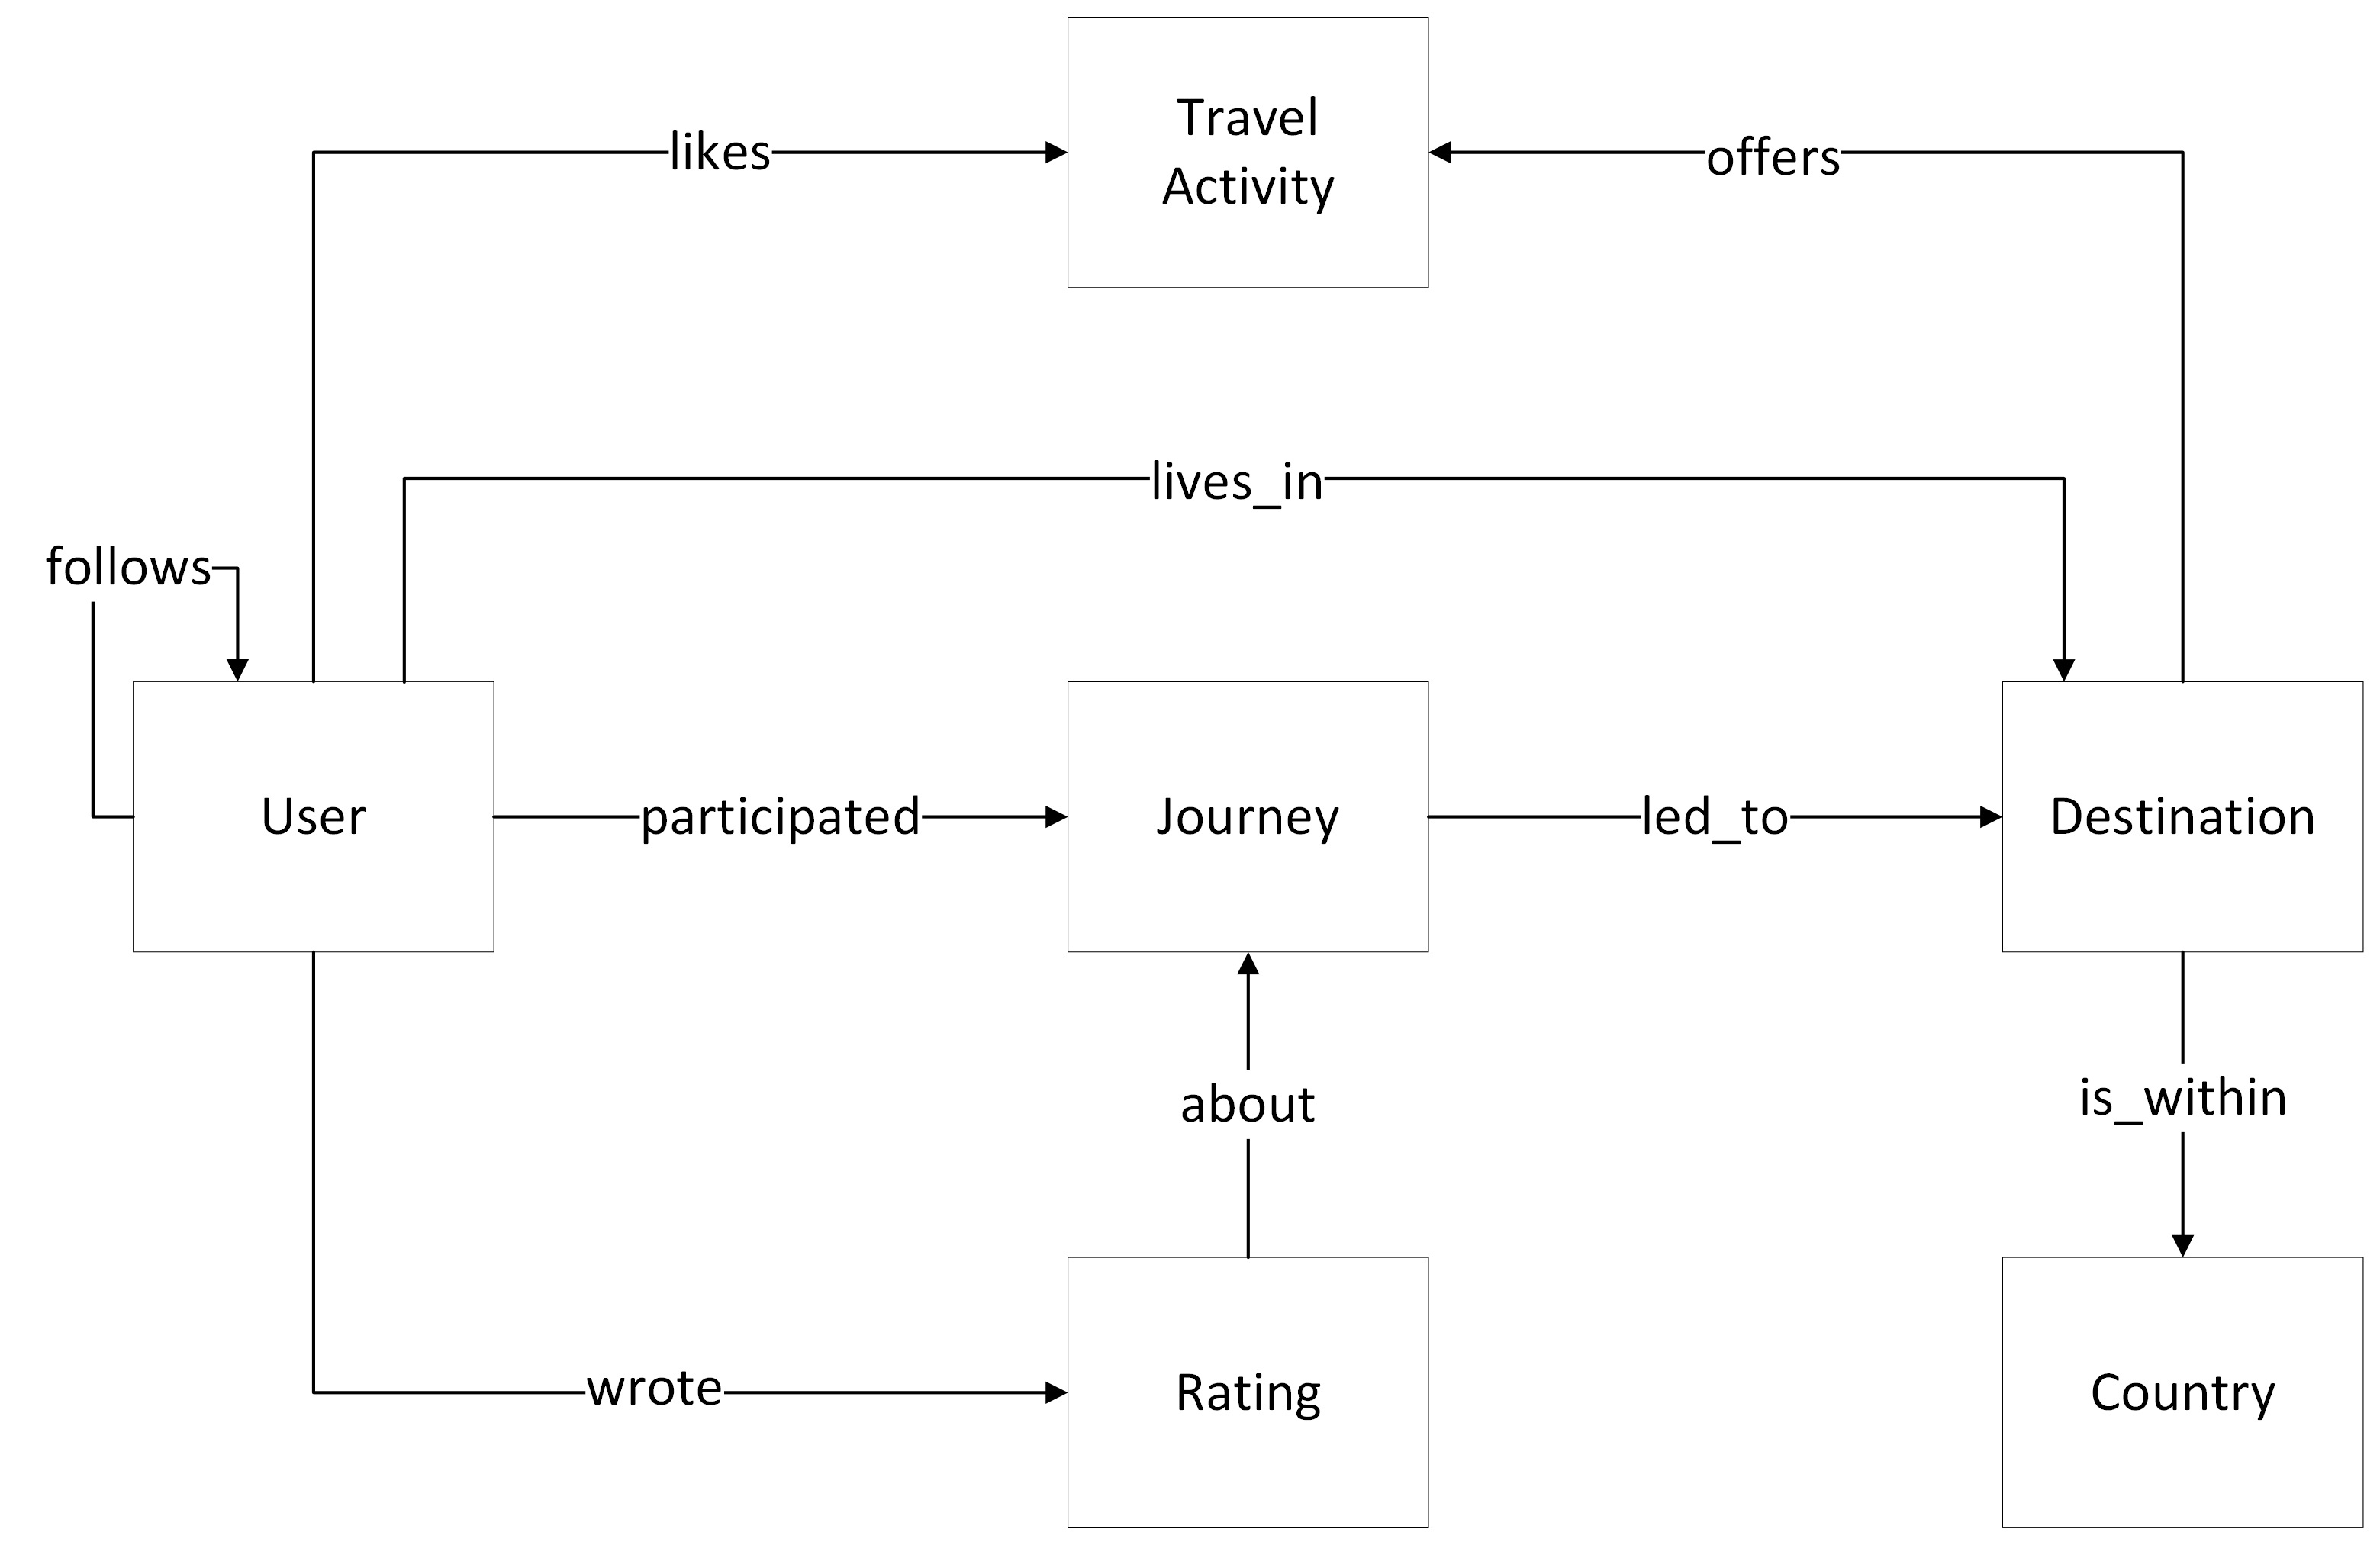
\includegraphics[width=\textwidth]{TravelEnthusiastNetwork-Conceptual}
	\caption[Konceptuální datový model.]{Konceptuální datový model pro sociální síť pro cestovní nadšence.}
	\label{fig:Concept}
\end{figure}

\subsection{Logický datový model}
V této fázi definujeme základní schéma, které bude určovat podobu našich dat v~databázi. Výstupem tedy bude schéma ve formě grafu nazývané \textit{logický datový model}, které bude mnohem detailnější než konceptuální datový model. Bude se zabývat detaily, kterými se zabývají vývojáři. Poté již můžeme do naší databáze vložit zkušební data a~vyzkoušet dotazy, které budou odpovídat na naše otázky načrtnuté v první části modelování dat.

\subsubsection{Vrcholové labely}
Podstatnou část práce již máme za sebou, neboť můžeme využít konceptuálního datového modelu a převést naše entity na vrcholové labely. Label vrcholu $u$ určuje, do~které skupiny vrcholů vrchol $u$ patří. Label pak můžeme používat v~dotazech na databázi a pracovat tak s různými skupinami vrcholů a dosáhnout tak lepšího výkonu při dotazování. Pro lepší pochopení je zde obrázek \ref{fig:VertexLabels}.

\begin{figure}[h]
	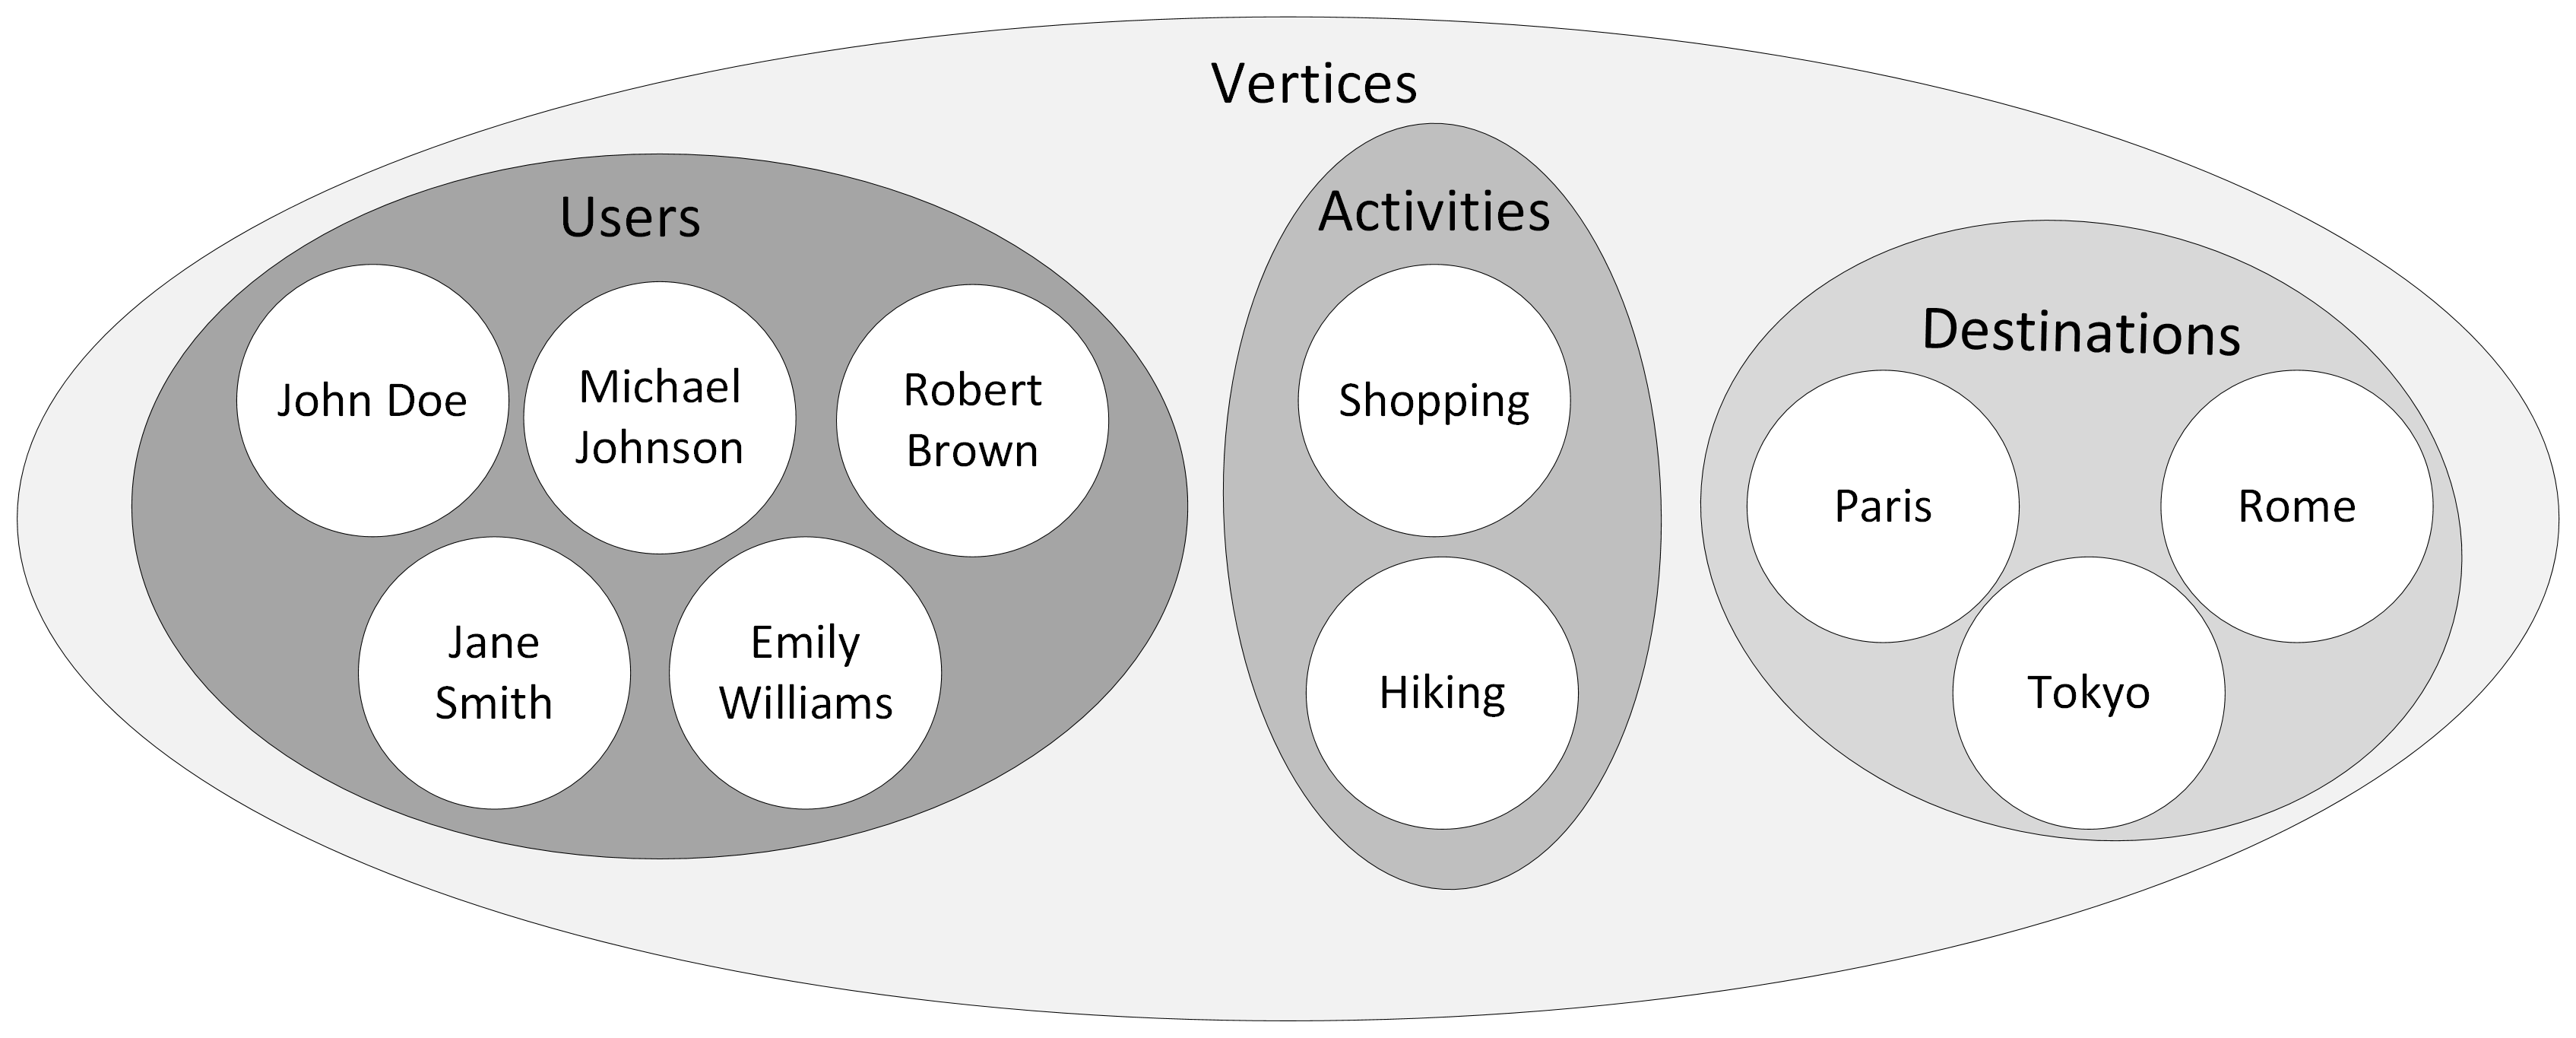
\includegraphics[width=\textwidth]{VertexLabels}
	\caption[Label vrcholu.]{Label vrcholu definuje, do které kategorie vrchol spadá.}
	\label{fig:VertexLabels}
\end{figure}

Labely vrcholů by měly být stručné a výstižné. Musíme mít na paměti budoucí rozšířitelnost aplikace a fakt, že s databází může pracovat jiný vývojář. Při přiřazování labelu je též vhodné zvolit co nejvíce obecný název, aby nám umožnil snadnou reprezentaci podobných objektů v budoucnu.

Povolený počet labelů pro jeden vrchol se u různých grafových databází liší. Jednou z možností je každému vrcholu přiřadit právě jeden label. To je například přístup ArangoDB databáze. Často se ale také hodí mít labelů více a pomocí nich umět vyjádřit dědičnost. Vrcholy pak spadají do více skupin vrcholů naráz. Tento přístup podporuje databáze Neo4j. Příkladem může být systém pro správu zaměstnanců a klientů ve firmě. Kromě vrcholových labelů \textit{Zaměstnanec} a \textit{Klient} použijeme také label \textit{Osoba}. Neboť zaměstnanec, reprezentovaný vrcholem v~databázi, jistě sdílí s klientem osobní údaje, jako jsou jméno a datum narození, ale může mít nějaké dodatečné informace, jako je například plat, nebo identifikační číslo zaměstnance. Nyní jednoduše můžeme vybrat data týkající se pouze klientů, ale zároveň můžeme požádat databázi o informaci o všech lidech spravovaných v~databázi. Příklad přiřazení více labelů jednomu vrcholu je znázorněn na obrázku \ref{fig:MoreVertexLabels}.

\begin{figure}[h]
	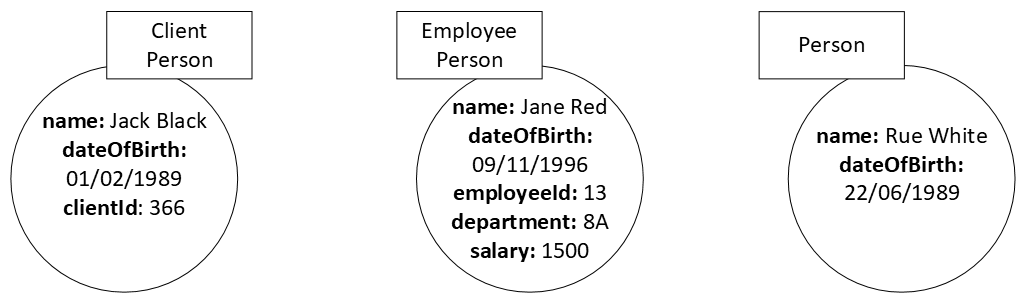
\includegraphics[width=\textwidth]{MoreVertexLabels}
	\caption{Jeden vrchol s více labely.}
	\label{fig:MoreVertexLabels}
\end{figure}

Častou chybou při navrhování labelů je nekonzistentní pojmenovávací konvence. Proto je dobré si stanovit pojmenovací konvenci, kterou se budeme řídit. V~našich příkladech je zvolena konvence doporučená v dokumentaci databáze Neo4j a tedy pro labely vrcholů budeme používat \textit{UpperCamelCase} notaci, pro labely hran \textit{SCREAMING\_SNAKE\_CASE} notaci s použitím podtržítka pro oddělení slov a pro vlastnosti \textit{camelCase} notaci. Labely vrcholů a názvy vlastností budou v jednotném čísle.

\subsubsection{Hranové labely}
Při hledání hran využijeme vztahů mezi entitami v připraveném konceptuálním datovém modelu. Podobně jako u vrcholových labelů musíme zvážit labely hran, jejichž názvy by opět měly dodržovat podobné principy. Navíc bychom se měli držet jedné dobré zásady. Přečtením labelů počátečního vrcholu, hrany z něj vycházející a~cílového vrcholu do nějž hrana vstupuje by nám mělo dávat vcelku smysluplnou větu. Příkladem by mohla být věta \uv{Uživatel napsal hodnocení.}, která vznikla spojením vrcholového labelu \textit{Uživatel}, hranového labelu \textit{NAPSAL} a labelu cílového vrcholu \textit{Hodnocení}. Ve většině případů mají věty tvar podle následující posloupnosti větných členů -- podmět-přísudek-předmět. Hrany mají obecně jeden label, někdy označovaný jako \textit{typ} hrany.

Vytvořené věty nám určují i orientaci hran. Opačná orientace hrany by ve většině případů způsobila, že přečtením daných labelů bychom dostali nesmyslnou větu. Pokud bychom tedy požadovali opačnou orientaci hran, museli bychom přistoupit ke změně labelu hrany. Orientace hrany by měla reflektovat to, jak přirozeným způsobem přemýšlíme o datech v naší doméně. Při procházení grafu není orientace hran překážkou. Dotazovací jazyky umožňují pomocí grafových vzorů procházet hrany v obou směrech.

Nyní zbývá ještě určit \textit{jedinečnost} hran. Jedinečnost lze definovat jako počet hran se stejným labelem mezi dvěma vrcholy. Tyto vrcholy mohou a nemusí mít stejný label. Jedinečnost hran se dělí na dva typy: \textit{jednoduchá} a \textit{vícenásobná}. Jednoduchá jedinečnost znamená, že mezi dvěma vrcholy existuje nejvýše jedna hrana se stejným labelem. Vícenásobná povoluje takových hran více.

Všechny hrany v naší aplikaci, až na jednu výjimku, budou mít jedinečnost jednoduchou. Neboť například vztah \textit{LÍBÍ\_SE} mezi daným uživatelem a cestovatelskou aktivitou lze vyjádřit pomocí existence jedné hrany mezi těmito dvěma vrcholy. Výjimkou je hrana s labelem \textit{VEDLA\_DO}. Jistě totiž může existovat situace, kdy v rámci cesty uživatel do dané destinace zavítá vícekrát a s touto možností by náš model měl také počítat. Tedy tato hrana bude mít vícenásobnou jedinečnost. Tyto hrany pak od sebe rozlišíme pomocí vlastností, které budou určovat období, kdy se daný uživatel v dané destinaci nacházel. Hrany s~mnohonásobnou jedinečností bychom měli rozlišovat pomocí vlastností, aby byly rozlišitelné.

Zvolení správné jedinečnosti hran je klíčové pro správné chování databáze. Pokud zvolíme jednoduchou jedinečnost tam, kde by měla být vícenásobná, databáze může vracet méně dat než očekáváme. Naopak, vícenásobná jedinečnost hran tam, kde by měla být jednoduchá, může vést k duplikativním datům. Každá hrana navíc zvyšuje čas výpočtu a komplikuje průchod grafem.

U některých implementací grafových databází, jako například JanusGraph, lze tuto jedinečnost vynutit při definování schématu. U implementací bez schématického přístupu, jako je Neo4j, tuto jedinečnost lze ošetřit pouze v rámci aplikace.

\subsubsection{Vlastnosti}
Poslední zastávkou při konstruování logického modelu jsou vlastnosti. V grafových databázích mohou mít vlastnosti vrcholy i hrany. Základní prvky grafu máme, ale chybí nám způsob jak rozlišit jednotlivé vrcholy (a někdy i~hrany) se~stejným labelem. K tomu nám slouží vlastnosti.

Vlastnosti v grafové databázi jsou páry klíč-hodnota a popisují konkrétní atributy hrany nebo vrcholu. Hodnota vlastnosti může být různého datového typu, například řetězec, číslo, pravdivostní hodnota nebo datový typ pro uchování datumu a času. Někdy též může být hodnota typu pole nebo seznam. Zde záleží na konkrétních implementacích. Jednou z~vlastností bývá námi definovaný unikátní identifikátor každého vrcholu, díky kterému přistupujeme ke konkretním vrcholům.

K dokončení logického modelu nám tedy zbývá najít a správně přiřadit potřebné vlastnosti konkrétním vrcholovým a hranovým labelům, rozumně je pojmenovat a určit jejich datový typ. K jejich nalezení nám opět mohou pomoci otázky z podkapitoly \ref{sec:problem-definition}.

\subsubsection{Logický datový model}
Naše výsledné grafové schéma popisuje obrázek \ref{fig:Schema}. Vrcholové labely jsou uvedeny v kroužcích. Hranové labely jsou vepsány do šipek. Vlastnosti vrcholů a hran jsou zobrazeny v obdélnících nacházejících se u vrcholů a na hranách. Za každou vlastností je v závorce uveden datový typ.

\begin{figure} [h]
	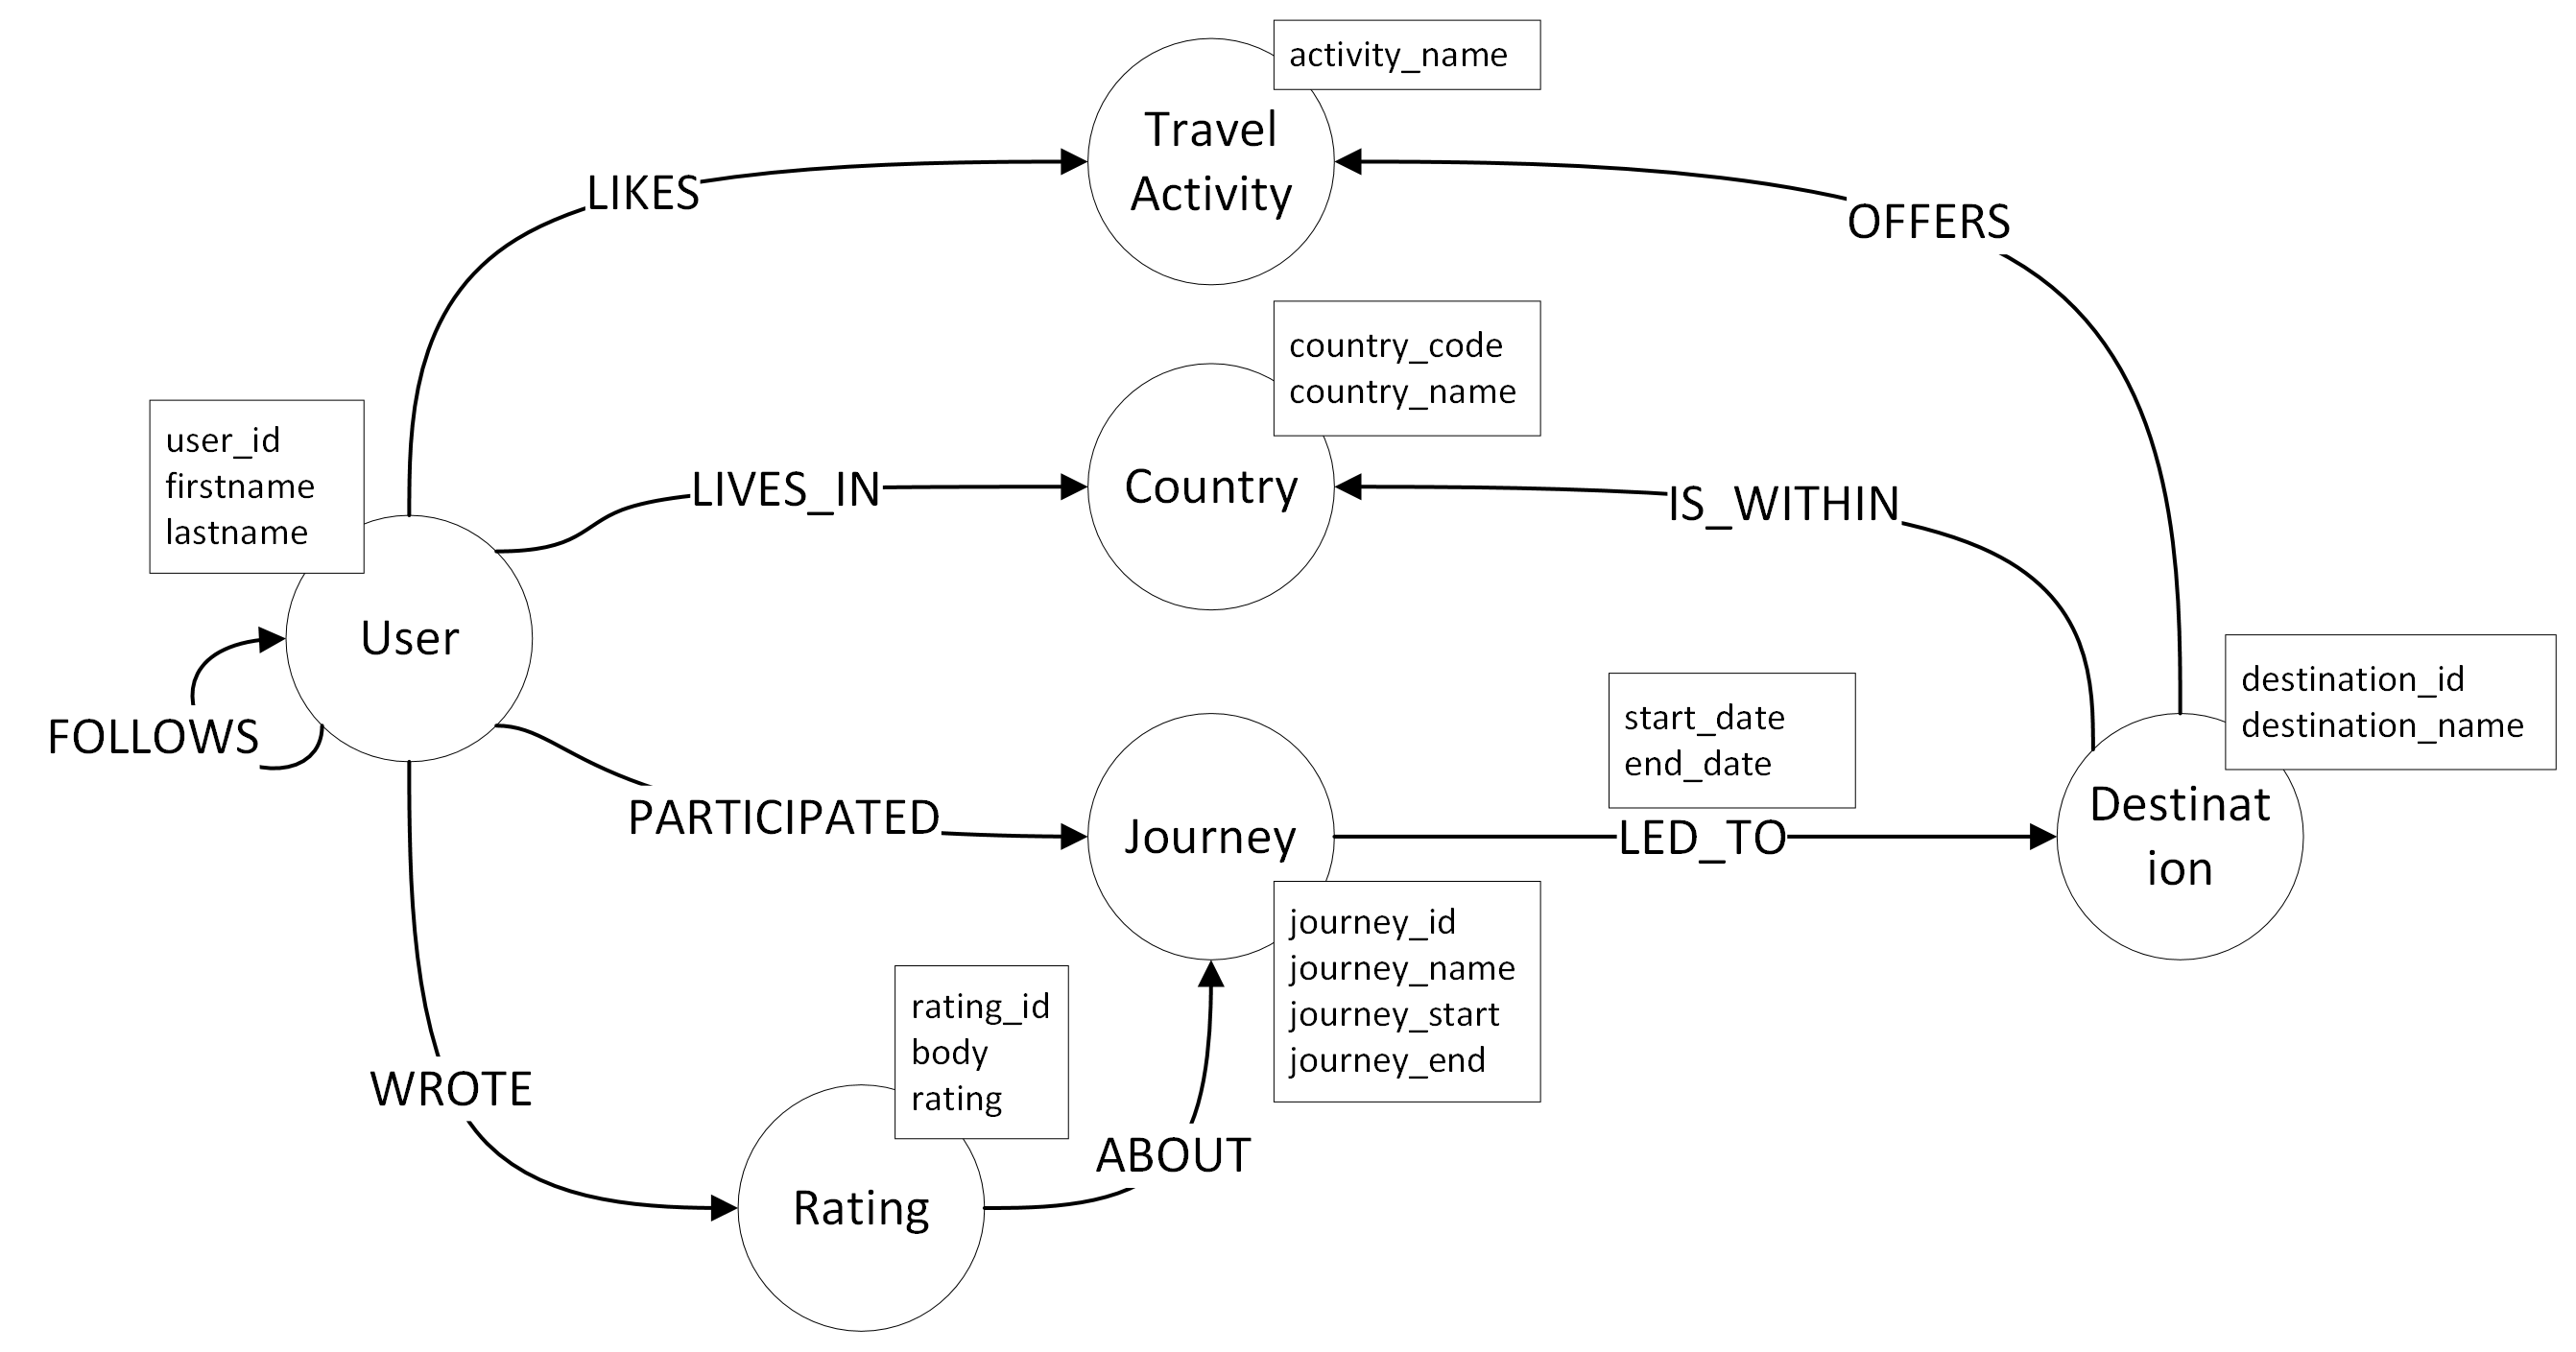
\includegraphics[width=\textwidth]{TravelEnthusiastNetwork-Graph}
	\caption[Logický datový model.]{Logický datový model pro sociální síť pro cestovní nadšence.}
	\label{fig:Schema}
\end{figure}

\subsection{Testování modelu}
Testování našeho grafového modelu spočívá ve vyzkoušení, zda se chová dle našeho očekávání (databáze vrací očekávané výsledky) a dotazování není moc pomalé ani pro velké množství dat. K testování lze využít široké škály nástrojů, které dotazovací jazyky a databáze nabízejí.

\subsubsection{Unit testy}
Při testování správnosti dotazů je vhodné použít \textit{unit testy}. Tedy vytvoříme si pro každý dotaz malé množství testovacích dat (například kolem 10 vrcholů, tak abychom z něj pouhým okem vyčetli správnou odpověď), kterými otestujeme správnost odpovědí z databáze. Příkladem unit testu je zdrojový kód \ref{kod:UnitTest}. Tento kód vloží do databáze data, která tvoří graf znázorněný na obrázku \ref{fig:UnitTest-Graph}. Následně zkontroluje dotaz hledající všechny uživatele, které mají od uživatele s vlastností \texttt{userId} rovnou 1 vzdálenost rovnou 2. Vidíme, že po spuštění testu databáze by měla vrátit uživatele s identifikátory 4 a 5. Následně po sobě uklidíme. Smažeme testovací data.

\begin{listing}[h]
\begin{minted}{cypher}
// Vytvoření testovacích dat
CREATE (u1:User {userId: 1, firstName: "John", lastName: "Doe"})
CREATE (u2:User {userId: 2, firstName: "Lisa", lastName: "Fog"})
CREATE (u3:User {userId: 3, firstName: "Bob", lastName: "John"})
CREATE (u4:User {userId: 4, firstName: "Jane", lastName: "Doe"})
CREATE (u5:User {userId: 5, firstName: "Paul", lastName: "Bae"})

CREATE (u1)-[:FOLLOWS]->(u2)
CREATE (u2)-[:FOLLOWS]->(u3)
CREATE (u1)-[:FOLLOWS]->(u3)
CREATE (u2)-[:FOLLOWS]->(u4)
CREATE (u3)-[:FOLLOWS]->(u5)

// Spuštění testu
MATCH (u:User {userId: 1})-[:FOLLOWS]->(u2)-[:FOLLOWS]->(u3)
WHERE NOT EXISTS((u)-[:FOLLOWS]->(u3)) AND u3 <> u
RETURN u3;

// Smazání testovacích dat
MATCH (u:User) WHERE u.userId IN [1, 2, 3, 4, 5]
DETACH DELETE u;
\end{minted}
\caption{Unit test}
\label{kod:UnitTest}
\end{listing}

\begin{figure}[h!]
	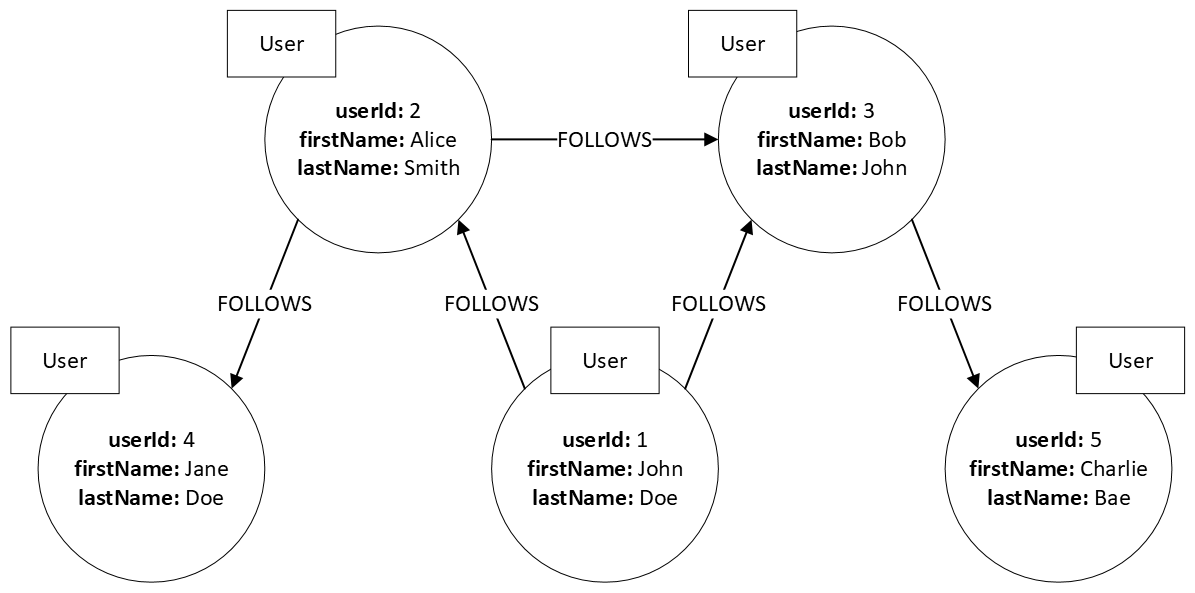
\includegraphics[width=\textwidth]{UnitTest-Graph}
	\caption[Unit test]{Graf vytvořený pomocí zdrojového kódu \ref{kod:UnitTest}.}
	\label{fig:UnitTest-Graph}
\end{figure}

\subsubsection{Profile a Explain}
Pokud čelíme pomalému vykonávání některých dotazů, můžeme použít dva nástroje pro diagnostiku problémů. První z nich se nazývá \textit{explain} a slouží pro vysvětlení, jak se bude průchod grafem vyvíjet na základě našeho dotazu. Používá se v situacích, kdy chceme zjistit chování průchodu grafem, ale nechceme jej vykonat. Výsledkem je optimalizovaný exekuční plán daného dotazu, který by byl vykonán na datech.

\pagebreak
Druhému říkáme \textit{profile} a podle dodaného dotazu profiluje, co průchod grafem udělal. Profile je hojně používaným nástrojem pro analýzu dotazů, neboť dotazy jsou často pomalé pouze pro několik vrcholů (například superuzlů). Toho lze využít k porovnání chování rychlých a pomalých vykonání dotazu. Získané informace pak využijeme k optimalizování našich dotazů.

\subsubsection{Indexy}
Při psaní této podkapitoly jsem čerpal též ze zdroje \cite{macrometa}. Pro efektivní hledání dat v rámci grafu lze použít \textit{indexy}. Toho lze využít pro vylepšení dotazů, neboť díky nim můžeme zrychlit průchod grafem, přístup ke konkrétním datům a další operace pracující s daty. Stanovením indexu se v databázi vytvoří datová struktura s efektivním hledáním obsahující redundantní kopii vybraných dat podle zadaných kritérií.

Indexy jsou výhodné pro data, která jsou častým terčem hledání. Nejčastěji se jedná o vlastnosti, které často vystupují ve filtrování dat v~dotazu, nebo identifikátory vrcholů. Dále se využívají pro vlastnosti, na kterých jsou prováděny různé operace s řetězci. Příkladem je hledání slov, které začínají na určitý podřetězec.

Indexy však také mají nevýhody. Zvýšují nároky na úložný prostor a mohou zpomalovat zápisy do databáze. Měly by tedy být vytvářeny pouze pro vlastnosti, pro které budou výhodné.

\subsubsection{Denormalizace}
\textit{Denormalizace} je metoda, která do databáze přidává redundantní data za účelem zrychlení čtení dat. Denormalizace v grafových databázích většinou znamená kopírování hodnot vlastností vrcholů na incidentní hrany. Často se jedná o časové informace. Nevýhodou tohoto procesu je nutná udržba těchto kopií což vede ke~zpomalení zápisů. Denormalizace je tedy vhodná pouze pro aplikace, kde počet operací pro čtení z databáze mnohonásobně převyšuje počet operací pro zápis.

\subsection{Ukázky dotazů}
V této podkapitole jsou ukázány tři zdrojové kódy \ref{kod:recommendation}, \ref{kod:substring} a \ref{kod:favouriteMonth} pro dotazy odpovídající na některé otázky z podkapitoly \ref{sec:problem-definition}. Výsledky dotazů jsou v tabulkách \ref{tab:recommendation}, \ref{tab:substring} a \ref{tab:favouriteMonth}. U dotazů, které vracejí více než tři výsledky, jsou uvedeny pouze první tři. Desetinná čísla ve výsledcích jsou zaokrouhlena na 3 desetinná místa.

\begin{listing}[h]
\begin{minted}{cypher}
MATCH (a:TravelActivity)
WHERE a.activityName IN ["Sightseeing", "Water Sports"]
WITH collect(a) AS activities
MATCH (d:Destination)
WHERE ALL(a IN activities WHERE (d)-[:OFFERS]->(a))
AND NOT exists ( (:User {userId: 10})-[]->(:Journey)-[]->(d) )
OPTIONAL MATCH (d)<-[:LED_TO]-()<-[:ABOUT]-(r:Rating)
WITH d, coalesce(avg(r.rating), "not rated") as rating
RETURN d.destinationName AS name, rating
ORDER BY rating DESC
LIMIT 3;
\end{minted}
\caption[Ukázka dotazu v Cypheru]{Dotaz v Cypheru odpovídající na zadání \uv{Najdi 3 nejlépe hodnocené destinace, které jsem nenavštívil, nabízející konkrétní cestovní aktivity.}}
\label{kod:recommendation}
\end{listing}

\begin{table}[h]
\begin{center}
\caption[Tabulka výsledků pro ukázkový dotaz]{Výsledná tabulka pro dotaz ve zdrojovém kódu \ref{kod:recommendation}.}
\label{tab:recommendation}
\begin{tabular}{ | l | c | }
 \hline
 \textbf{name}  & \textbf{rating} \\
 \hline \hline
 Dallas & 4,222 \\
 Bangkok & 4,077 \\
 San Antonio & 3,905 \\
 \hline
\end{tabular}
\end{center}
\end{table}

\begin{listing}[h]
\begin{minted}{SQL}
FOR u IN User
    FILTER CONTAINS(UPPER(u.firstName), UPPER("RoB"))
        OR  CONTAINS(UPPER(u.lastName), UPPER("RoB"))
    SORT u.firstName, u.lastName
    RETURN {userId: u._key, name: CONCAT(u.firstName, " ", u.lastName)}
\end{minted}
\caption[Ukázka dotazu v AQL]{Dotaz v AQL odpovídající na zadání \uv{Najdi uživatele, jejichž jméno nebo přijmení obsahuje specifikovaný řetězec.}}
\label{kod:substring}
\end{listing}

\begin{table}[h]
\begin{center}
\caption[Tabulka výsledků pro ukázkový dotaz]{Výsledná tabulka pro dotaz ve zdrojovém kódu \ref{kod:substring}.}
\label{tab:substring}
\begin{tabular}{ | l | c | }
 \hline
 \textbf{userId}  & \textbf{name} \\
 \hline \hline
 153 & Ashley Roberts\\
 146 & Kathryn Robbins\\
 71 & Marie Robertson\\
 \hline
\end{tabular}
\end{center}
\end{table}

\begin{listing}[h]
\begin{minted}{Groovy}
g.V().has("Destination", "destinationId", 7).
  inE("LED_TO").
  group().by(values("startDate").map{it.get().getMonth() + 1}).
  unfold().
  project("month", "rating").
    by(keys).
    by(select(values).unfold().
        outV().in('ABOUT').values('rating').mean().fold().
        coalesce(unfold(),constant('not rated'))).
  order().
    by(__.select("rating").map { it.get() instanceof Number ? 0 : 1 }).
    by(__.select("rating"), desc).
  limit(3)
\end{minted}
\caption[Ukázka dotazu v Gremlinu]{Dotaz v Gremlinu odpovídající na zadání \uv{Pro konkrétní destinaci vrať 3 měsíce v roce, ve kterých je nejlépe hodnocená.}}
\label{kod:favouriteMonth}
\end{listing}

\begin{table}[h]
\begin{center}
\caption[Tabulka výsledků pro ukázkový dotaz]{Výsledná tabulka pro dotaz ve zdrojovém kódu \ref{kod:favouriteMonth}.}
\label{tab:favouriteMonth}
\begin{tabular}{ | l | c | }
 \hline
 \textbf{month}  & \textbf{rating} \\
 \hline \hline
 5 & 3,25 \\
 3 & 2,625 \\
 1 & not rated \\
 \hline
\end{tabular}
\end{center}
\end{table}

\clearpage
\section{Cestování v grafu}
V této kapitole se zaměříme na velkou výhodu grafových databází -- cestování v~grafu. To může být rozděleno na dva podproblémy: cestování v grafu, kde dopředu známe grafový vzor a cestování v grafu, kde dopředu grafový vzor neznáme. Ne vždy totiž platí, že cestu mezi dvěma vrcholy známe. Často máme pouze počáteční a cílový vrchol a chceme například zjistit, zda je jeden z druhého dosažitelný.

Pro ukázkové příklady v podkapitolách \ref{sec:unweightedPath} a \ref{sec:weightedPath} je použitý dataset \cite{railNetworkDataset} obsahující informace o belgických železničních stanicích a jednosměrných spojeních mezi nimi. K němu příslušný logický datový model ukazuje obrázek \ref{fig:RailNetwork-Graph}. Původní dataset je rozdělen do dvou \texttt{csv} souborů. Jeden uchovává informace o železničních stanicích a~druhý spojení mezi nimi. Informace obsahující souřadnice pro hrany byly vypuštěny. Seznam souborů shrnuje tabulka \ref{tab:RailNetwork-csv}.

\begin{table}[h]
\caption{Použité soubory pro ukázku hledání cest.}
\label{tab:RailNetwork-csv}
\begin{tabularx}{\textwidth}{ | l | c | c | X | }
 \hline
 \textbf{Typ} & \textbf{Název souboru} & \textbf{Počet řádků} & \textbf{Informace o souboru} \\
 \hline \hline
 Entity & \texttt{stations.csv} & 559 & Informace o železničních stanicích. \\
 \hline
 Vztahy & \texttt{leads\_to.csv} & 1385 & Stanice vede do stanice.\\
 \hline
\end{tabularx}
\end{table}

\begin{figure}[h]
\begin{center}
	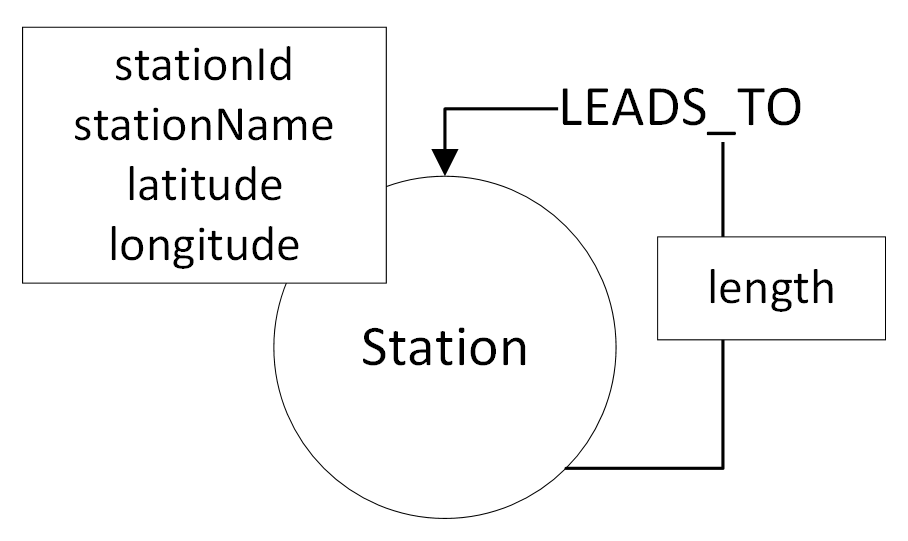
\includegraphics[scale=0.75]{RailNetwork-Graph}
	\caption[Grafový model pro ukázkové příklady.]{Logický grafový model pro ukázkové příklady v této kapitole.}
	\label{fig:RailNetwork-Graph}
\end{center}
\end{figure}

\subsection{Procházení grafu}
Pro prohledávání grafů od určitého počátečního vrcholu lze použít dva známé grafové algoritmy využívané při cestování v grafu:
\begin{enumerate}
  \item \textit{Prohledávání do šířky}, označované jako BFS (z anglického Breadth-First Search)
  \item \textit{Prohledávání do hloubky}, označované jako DFS (z anglického Depth-First Search)
\end{enumerate}
Oba algoritmy mají časovou složitost $O(|E| + |V|)$.

\subsubsection{Prohledávání do šířky}
Algoritmus BFS začne v počátečním vrcholu a následně prohledá všechny své sousední vrcholy. Poté projde sousedy sousedů počátečního vrcholu, které ještě nenavštívil a tak postupuje, dokud nenavštíví všechny dosažitelné vrcholy.

Tento způsob procházení grafu lze znázornit pomocí kořenového stromu. Kořenem je počáteční vrchol. Algoritmus prochází vrcholy grafu po jednotlivých úrovních tohoto stromu. Platí, že nejkratší cesta z počátečního vrcholu do vrcholu $v$ v neohodnoceném grafu má délku rovnou hloubce $v$ ve stromu, který průchodem vznikne. Proto bývá využíván při hledání nejkratších cest v neohodnoceném grafu. Lze jej efektivně implementovat pomocí fronty vrcholů. Průchod grafem do šířky a~strom, vzniklý průchodem algoritmu jsou znázorněny na obrázku \ref{fig:bfs}. Algoritmus začínal ve vrcholu B. Pořadí, ve kterém jsou vrcholy procházeny, je znázorněno čísly v obdélnících u každého vrcholu.

\begin{figure}[h]
	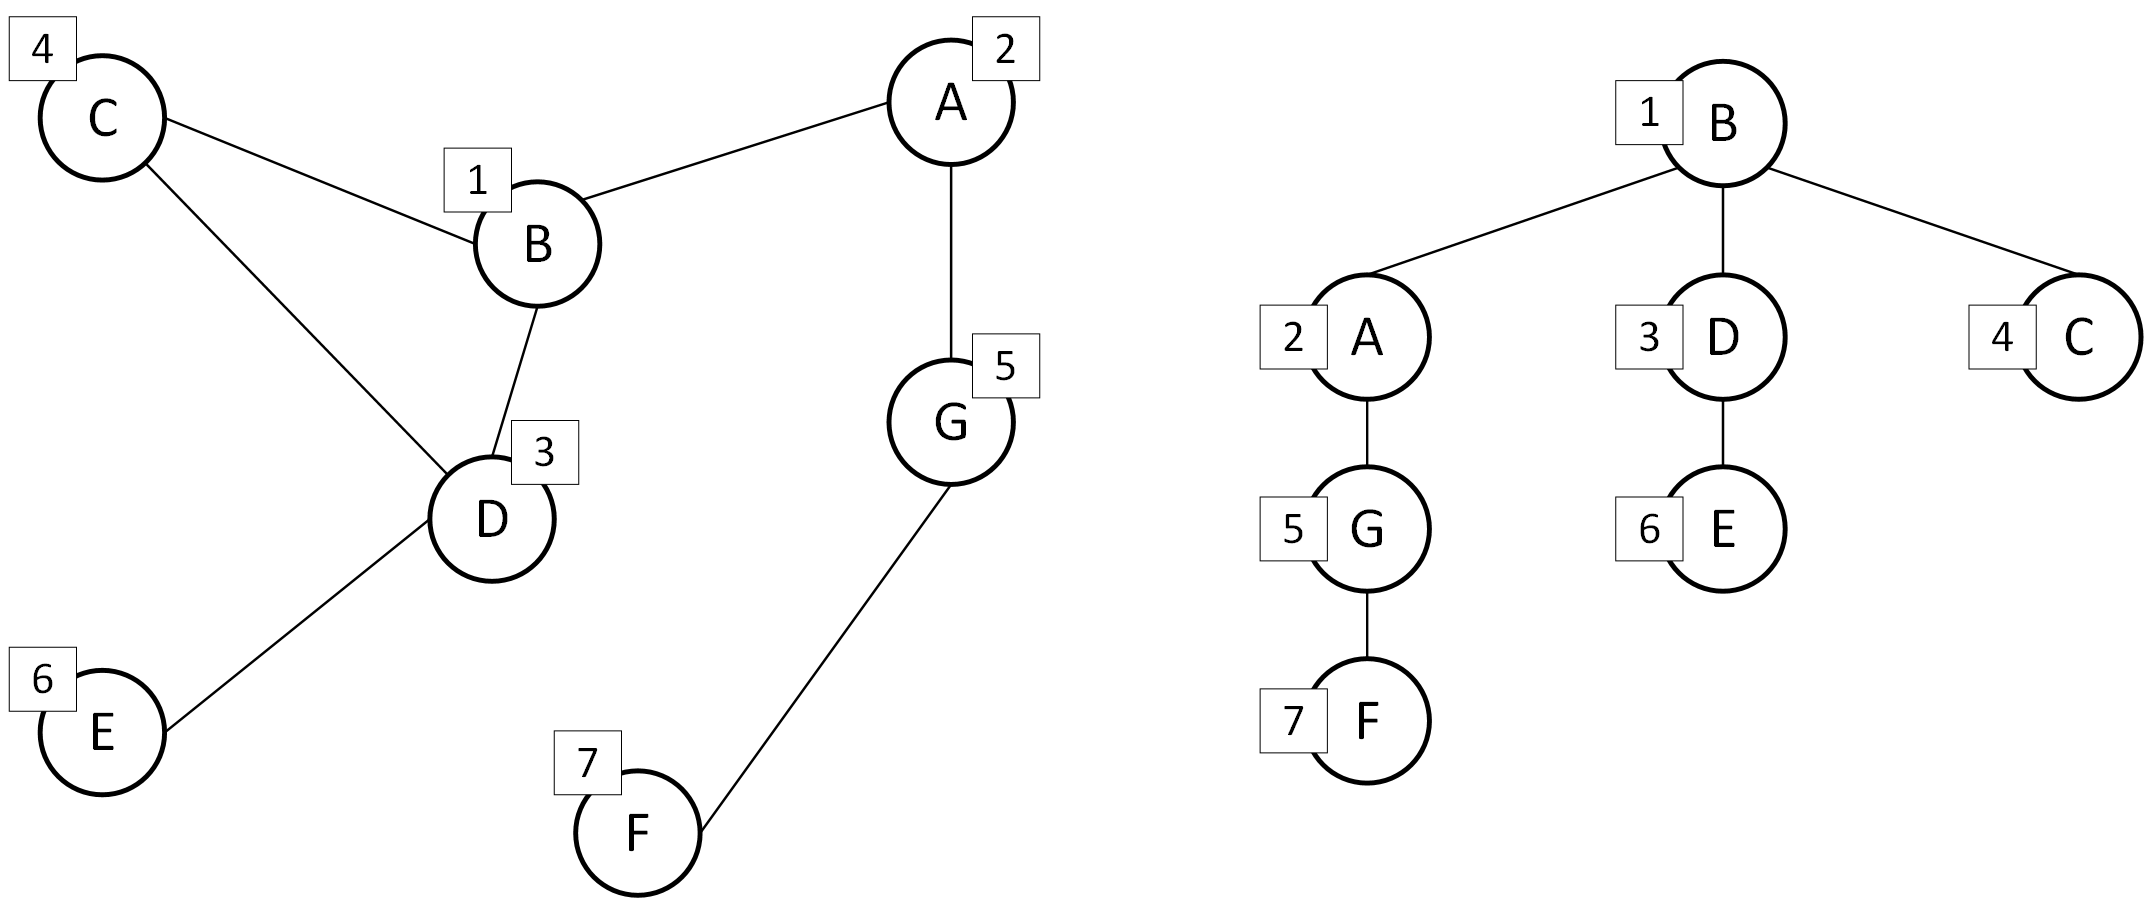
\includegraphics[width=\textwidth]{Bfs}
	\caption[Algoritmus prohledávání do šířky.]{Průchod algoritmu  BFS grafem.}
	\label{fig:bfs}
\end{figure}

\subsubsection{Prohledávání do hloubky}
Algoritmus DFS začíná v počátečním vrcholu. V aktuálně navštíveném vrcholu vždy přejde do dosud nenavštíveného souseda, pokud takový soused existuje, jinak provede backtracking -- vrací se zpět po cestě odkud přišel, dokud nenalezne vrchol jehož soused nebyl navštíven. Skončí, jakmile jsou všechny dosažitelné vrcholy navštíveny.

Tento způsob procházení grafu lze opět znázornit pomocí kořenového stromu, kde kořen je počáteční vrchol. Pozorování ohledně nejkratších cest, jaké jsme udělali u BFS, v tomto stromu obecně neplatí. DFS je výhodný pro předdefinovanou cestu, neboť není tak náročný na paměť. Při implementci využíváme zásobník. Průchod grafem do hloubky a strom, vzniklý průchodem algoritmu jsou znázorněny na obrázku \ref{fig:dfs}. Algoritmus začínal ve vrcholu B. Pořadí, ve kterém jsou vrcholy procházeny, je znázorněno čísly v obdélnících u každého vrcholu.

\begin{figure}[h]
	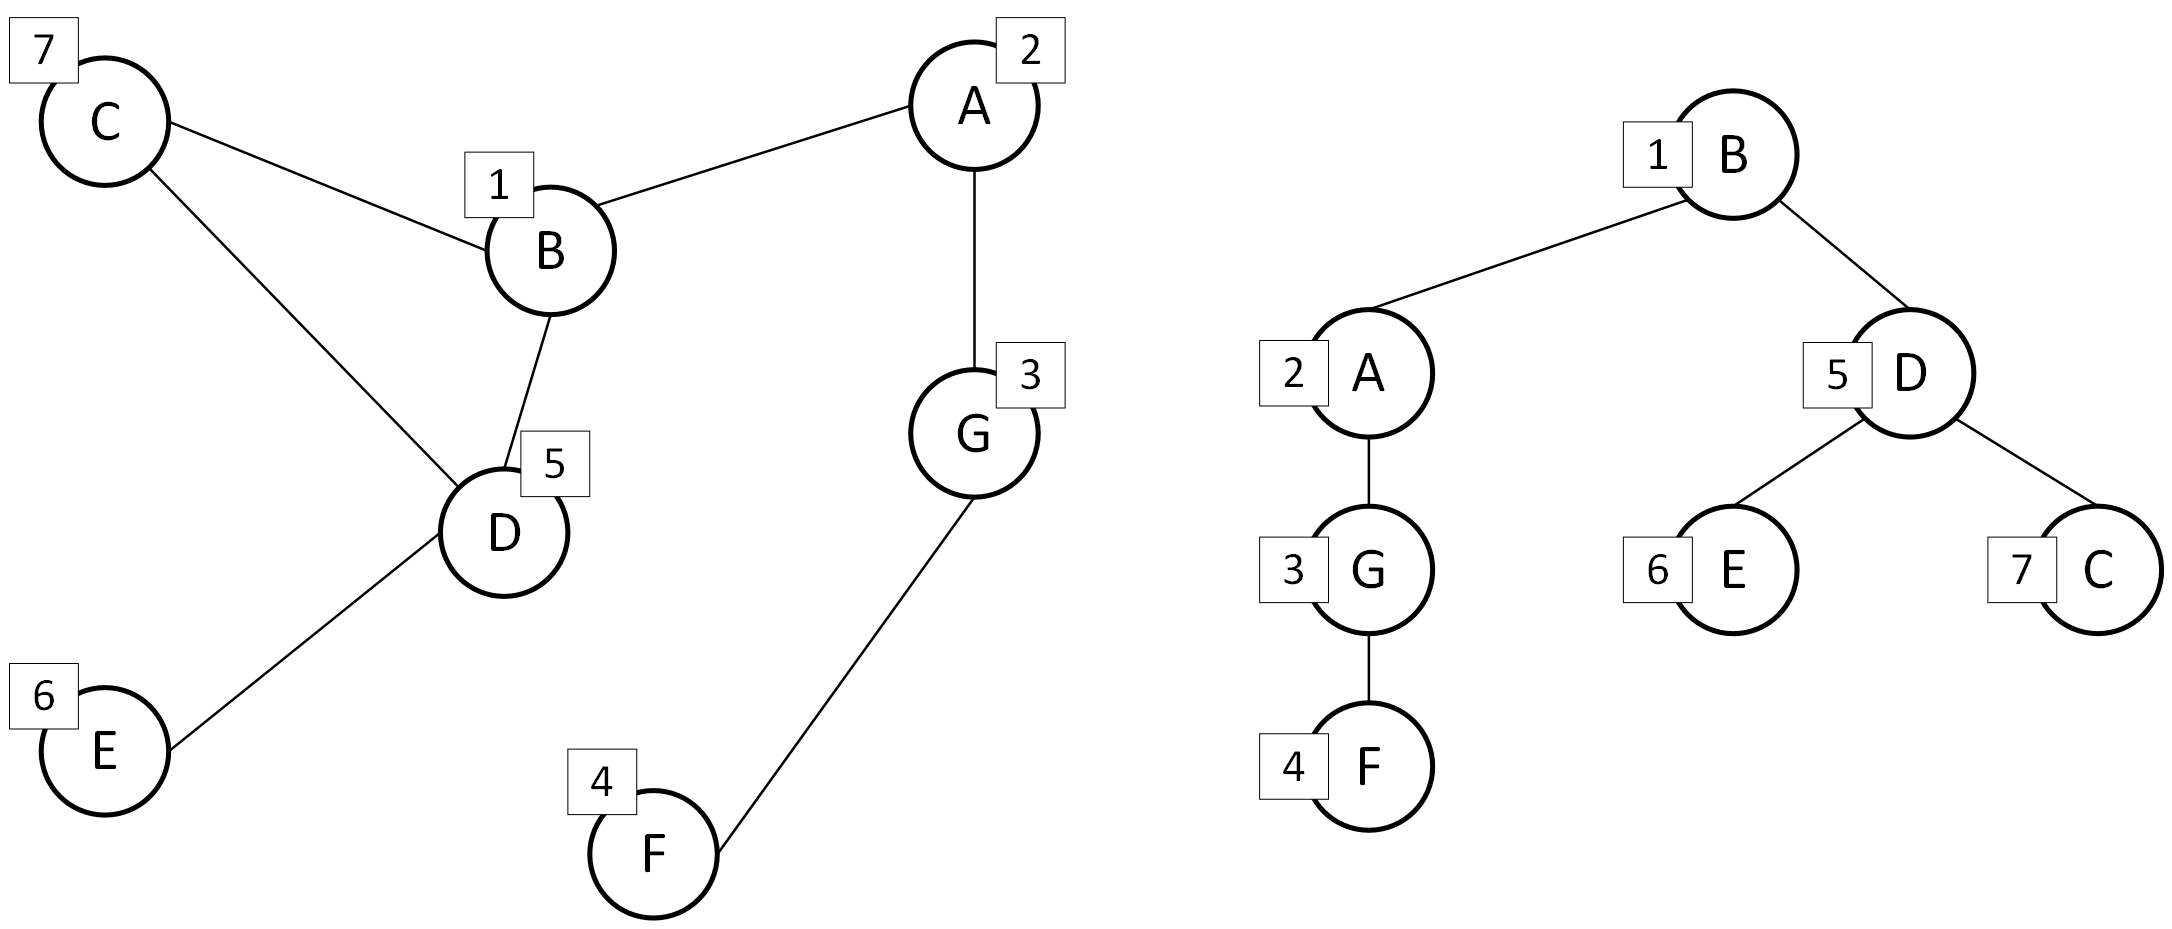
\includegraphics[width=\textwidth]{Dfs}
	\caption[Algoritmus prohledávání do hloubky.]{Průchod algoritmu DFS grafem.}
	\label{fig:dfs}
\end{figure}

\subsection{Předdefinovaná cesta}
Často při průchodu grafem předem známe grafový vzor určující cestu, kterou musíme projít, abychom dosáhli požadovaných výsledků pro daný dotaz. Předem známe délku cesty a vrcholové a hranové labely, přes které cesta prochází. Tento průchod grafem budeme označovat jako \textit{předdefinovaná cesta}. V této podkapitole se vrátíme k naší aplikaci pro cestovatelské nadšence s logickým datovým modelem na~obrázku \ref{fig:Schema}. Při překladu otázek na dotazy zjistíme, že všechny grafové vzory z těchto otázek odvozené představují předdefinovanou cestu.

\subsubsection{Ukázka předdefinované cesty}
Příkladem může být dotaz odpovídající na otázku \uv{Které destinace navštívil uživatel s identifikátorem X?}. Vidíme, že v dotazu budou jistě figurovat dvě entity: \textit{Uživatel} a \textit{Destinace}. Při pohledu na logický datový model je zřejmé, že abychom dostali všechny navštívené destinace pro konkrétního uživatele, musíme v grafu projít i přes všechny vrcholy s labelem \textit{Cesta}, které uživatel podniknul. Tyto vrcholy spojují uživatele s destinacemi, které navštívil. Jedná se tedy o~předdefinovanou cestu, neboť víme, že musíme provést cesty o délce 2 obsahující vrcholy s labely \textit{Uživatel}, \textit{Cesta} a \textit{Destinace}.

Nyní je otázkou, v kterých vrcholech je dobré průchod začít. Volba počátečních vrcholů má často velký vliv na výsledný čas výpočtu. Jednou z možností je začít na vrcholech s labelem \textit{Destinace}. Grafový vzor by pak určoval cestu ze~všech vrcholů s labelem \textit{Destinace} přes hrany spojující tyto vrcholy s~vrcholy s~labelem \textit{Cesta}. Následně pro všechny vrcholy s labelem \textit{Cesta} zkontrolujeme, zda se jich vrchol s labelem \textit{Uživatel}, který má shodný identifikátor s X, zúčastnil. Destinace, které by takto nebyly s uživatelem spojeny, by byly vyfiltrovány. Vyhovující destinace by byly vráceny. Ačkoliv by tento výpočet vedl ke správnému výsledku, procházet přes všechny destinace a tedy i přes všechny cesty není nejvhodnější. Vrcholů, které bychom museli zkontrolovat, je zbytečně mnoho. Obdobně nevyhovující by bylo začínat ve vrcholech s labelem \textit{Cesta}.

Nejlepším řešením je začít ve vrcholu představujícím konkrétního uživatele. Následně projít přes vrcholy s labelem \textit{Cesta}, kterých se uživatel zúčastnil a~dostat se tak ke všem destinacím, které daný uživatel navštívil. Obecně je doporučeno začínat v co nejmenším počtu vrcholů. Výsledný dotaz v Cypheru ukazuje zdrojový kód \ref{kod:VisitedDestinations}. Do odpovědi je zahrnuta též informace, kolikrát daný uživatel destinace navštívil. Výsledky jsou podle toho seřazeny.

\begin{listing}[h]
\begin{minted}{cypher}
WITH 3 AS id
MATCH (u:User {userId:id})-[:PARTICIPATED]->(:Journey)
	-[:LED_TO]->(d:Destination)
RETURN d.destinationName, COUNT(d) AS count
ORDER BY count DESC, d.destinationName ASC;
\end{minted}
\caption[Předdefinovaná cesta.]{Ukázka kódu dotazu využívajícího předdefinovanou cestu.}
\label{kod:VisitedDestinations}
\end{listing}

\subsection{Hledání cesty v neohodnoceném grafu}
\label{sec:unweightedPath}
Nyní se podíváme na hledání cesty v grafu, který je neohodnocený. Tyto cesty lze hledat i v grafu s ohodnocenými hranami tak, že ohodnocení hran ignorujeme. Počet hran na cestě pak určuje délku cesty.

Cest mezi dvěma vrcholy může být obrovské množství. Pokud neomezíme průchod grafem, například pomocí počtu hran na cestě, může se stát, že výpočet bude trvat velmi dlouho, nebo v horším případě bude nekonečný. Druhá možnost nastane pokud nezajistíme, že v grafu hledáme opravdu jen cesty a nikoliv sledy.

Důvodů pro hledání cesty mezi dvěma vrcholy může být vícero. Jedním z~nich je hledání cesty s nejkratší délkou. Dalšími je zjištění dosažitelnosti a hledání cesty o fixní délce.

Problém nejkratší cesty v neohodnoceném grafu lze vyřešit pomocí algoritmu BFS, neboť systematicky prochází všechny vrcholy, které mají vzdálenost od~počátečního vrcholu rovnou $k$, kde $ k \in \mathbb{N}_0 $. Začíná pro $ k = 0 $ a postupně v každém kroku $ k $ zvětšuje o 1. V každém kroku pak kontroluje všechny vrcholy $u$, které mají z počátečního vrcholu vzálenost rovnou $k$. Pokud narazí na cílový vrchol, vrací $k$, které představuje délku nejkratší cesty do daného vrcholu. Algoritmus si pro každý navštívený vrchol může pamatovat vrchol, ze kterého do něj přišel. Tímto způsobem může vrátit i konkrétní cestu, kterou se do vrcholu dostal. Nejkratších cest mezi dvěma vrcholy může být více. Pro libovolné $ m \in \mathbb{N} $ můžeme takto postupovat i~pro nalezení až $ m $ různých nejkratších cest pro dva dané vstupní vrcholy.

V databázi ArangoDB lze cesty mezi stanicemi obsahující 1 až 4 hrany najít pomocí dotazu ve zdrojovém kódu \ref{kod:unweightedPath}. Na řádku 2 vyfiltrujeme ty sledy, které obsahují cyklus a specifikujeme strategii prohledávání do šířky. Výsledky jsou seřazeny podle počtu hran na cestě. Tabulka \ref{tab:ShortestPath-Unweighted-Example} ukazuje výsledek tohoto dotazu po zavolání.

\begin{listing}[h]
\begin{minted}{SQL}
FOR v,e,p IN 1..4 OUTBOUND 'Station/157' LEADS_TO
OPTIONS {uniqueVertices: 'path', order: 'bfs'}
    FILTER p.vertices[-1]._id == 'Station/1061'
    LET distance = LENGTH(p.edges[*])
    LET stations = p.vertices[*].stationName
    SORT distance
    RETURN { 
        stations,
        distance
    }
\end{minted}
\caption{Cesty v neohodnoceném grafu.}
\label{kod:unweightedPath}
\end{listing}

\begin{table}[h]
\begin{center}
\caption[Tabulka výsledků]{Výsledná tabulka pro dotaz ve zdrojovém kódu \ref{kod:unweightedPath}.}
\label{tab:ShortestPath-Unweighted-Example}
\begin{tabular}{ | l | c | }
 \hline
 \textbf{stations}  & \textbf{distance} \\
 \hline \hline
 BILZEN, BOKRIJK, KIEWIT, SCHULEN & 3 \\
 BILZEN, DIEPENBEEK, HASSELT, SCHULEN & 3 \\
 BILZEN, BOKRIJK, KIEWIT, HASSELT, SCHULEN & 4 \\
 BILZEN, DIEPENBEEK, HASSELT, KIEWIT, SCHULEN & 4 \\
 BILZEN, DIEPENBEEK, HASSELT, ZONHOVEN, SCHULEN & 4 \\
 \hline
\end{tabular}
\end{center}
\end{table}

\subsection{Hledání cesty v ohodnoceném grafu}
\label{sec:weightedPath}
Délka cesty mezi počátečním a koncovým vrcholem v ohodnoceném grafu je dána součtem ohodnocení hran na cestě. Tedy nejmenší počet hran na cestě nutně neznamená, že součet ohodnocení hran je menší než na jiné cestě obsahující více hran.

Pro hledání nejkratší cesty v ohodnoceném grafu se nejčastěji využívá Dijkstrův algoritmus. Ve zdrojovém kódu \ref{kod:ShortestPath-Weighted-Example} z knihy \cite{practitioner} je ukázána verze Dijkstrova algoritmu pro hledání cesty mezi dvěma vrcholy napsaná v jazyce Gremlin. Dotaz najde nejkratší cestu mezi dvěma vrcholy v ohodnoceném grafu a vrátí jména stanic na této cestě, jejich počet a délku této cesty. Dijkstrův algoritmus je více popsán v následující kapitole. 

\begin{listing}[h]
\begin{minted}{groovy}
g.withSack(0.0).V().
    has("Station", "stationId", 1048).
    repeat(outE("LEADS_TO").
            sack(sum).by("length").
            inV().as("visited").
            simplePath().
            group("minDist").by().by(sack().min()).
            filter(project("currMinDist", "sackDist").
                    by(select("minDist").select(select("visited"))).
                    by(sack()).
                where("currMinDist", eq("sackDist")))).
    until(has("Station", "stationId", 810)).
    order().by(sack(), asc).
    limit(1).
    project("stations", "stationsCount", "totalLength").
        by(path().
            unfold().
            hasLabel("Station").
            values("stationName").
            fold()).
        by(path().count(local).math('(_+1)/2')).
        by(sack()).
    fold() 
\end{minted}
\caption[Nejkratší cesta v ohodnoceném grafu.]{Hledání nejkratší cesty v ohodnoceném grafu.}
\label{kod:ShortestPath-Weighted-Example}
\end{listing}

Zde obzvláště platí, že cest mezi dvěma vrcholy může být opravdu mnoho, hlavně ve velikých grafech. Proto se často z časových důvodů nejkratší cesta aproximuje. Například pokud při procházení grafu narazíme na superuzel, cestu přes něj nepočítáme, neboť bychom museli procházet jeho každou výstupní hranu, což by bylo výpočetně náročné.
\clearpage
\section{Algoritmy}

Tato kapitola byla napsána pomocí knih \cite{graphAlgorithms} a \cite{inAction}. Dále byla využita dokumentace knihovny Graph Data Science Library \cite{neo4jDoc} a zdroj \cite{disk}.

V této kapitole představíme několik užitečných algoritmů navržených pro práci s grafy. Tyto algoritmy jsou vhodné pro použití při dotazech na grafovou databázi a mohou být aplikovány v různých situacích. Používají je především OLAP systémy. Umožňují nám například efektivně hledat nejkratší cesty mezi vrcholy, nacházet vrcholy, které pro nás mohou být svým způsobem důležité, nebo třeba hledat skupiny navzájem propojených vrcholů v grafu. Tyto algoritmy a~mnohé další obsahuje knihovna s názvem \texttt{Graph Data Science Library}. Tuto knihovnu lze dodatečně nainstalovat do databáze Neo4j. Zkráceně ji budeme označovat \texttt{GDS}.

Pro nejefektivnější běh algoritmů používá \texttt{GDS} k reprezentaci dat grafu speciální formát grafu uložený dočasně v paměti. Jedná se o strukturu vrcholů a~hran, jejichž vlastnosti mohou být pouze číselné. Každý takový graf je pojmenován a~díky tomu na něj můžeme odkazovat v algoritmech. Tyto odkazy jsou uložené v \textit{grafovém katalogu}. Graf lze vytvořit více způsoby. V práci je použitý způsob vytvoření grafu pomocí \textit{Cypher projekce}.

Algoritmy pak mohou běžet ve třech režimech:
\begin{itemize}
\item \textit{Stream} -- výsledky algoritmu obdržíme jako výsledek dotazu.
\item \textit{Mutate} -- výstup algoritmu aktualizuje graf v paměti.
\item \textit{Write} -- zapíše výsledek algoritmu zpět do databáze Neo4j.
\end{itemize}

\subsection{Algoritmy pro hledání cesty v grafu}
V praxi je užitečné v grafu najít rychle optimální cestu mezi dvěma, či více vrcholy. Tento problém potřebují řešit například nástroje pracující s grafy reprezentující mapy, které hledají vhodné trasy mezi body na mapě. Dalšími příklady optimalizační problémů jsou řízení dodavatelských řetězců, hledání nejvhodnějšího autobusového spojení a analýza počítačové sítě. Pro řešení tohoto problému vznikly různé algoritmy. Každý pracuje odlišně a je výhodný pro různé poddruhy problémů. Dva z nich si zde představíme.

\subsubsection{Dijkstrův algoritmus}
Při psaní této podkapitoly jsem čerpal převážně ze zdroje \cite{disk}. Dijkstrův algoritmus\cite{dijkstra-original} je jeden z nejznámějších algoritmů pro hledání nejkratší cesty. Lze jej aplikovat na~neohodnocené grafy, nebo grafy s kladným ohodnocením hran. Jedná se o~hladový algoritmus, který vychází z daného vrcholu a~hledá nejkratší cesty ke~všem ostatním vrcholům v grafu. Lze jej také omezit, aby iteroval jen dokud nenajde nejkratší cestu ke konkrétnímu cílovému vrcholu. Správné řešení je dosáhnuto díky pamatování si dosud nejkratších nalezených cest do již navštívených vrcholů. V každé iteraci se pak vybere jeden vrchol s~nejkratší nalezenou cestu ze všech vrcholů, které ještě nebyly zpracovány. Poté se aktualizují všechny nejkratší cesty do jeho sousedů, pokud cesta přes tento vybraný vrchol představuje zlepšení. Pokud je nějaký vrchol nedosažitelný nebo ještě nebyl navštívený, má hodnotu $\infty$.

Nevýhodou tohoto algoritmu je, že pro nalezení nejkratší cesty mezi dvěma zadanými vrcholy je v nejhorším případě potřeba nalézt všechny nejkratší cesty do ostatních vrcholů, než se algoritmus dostane k požadovanému výsledku. To nastává v případě, kdy je mezi danými vrcholy nejkratší cesta nejdelší ze všech nejkratších cest z počátečního vrcholu do ostatních vrcholů. Dijkstrův algoritmus navíc nefunguje v grafu, kde se vyskytují hrany se záporným ohodnocením. V těchto grafech je proto nutné použít jiný algoritmus -- například Bellman-Fordův\cite{bellman-original} algoritmus.

\subsubsection{Algoritmus A*}
Při psaní této podkapitoly jsem čerpal též ze zdroje \cite{astar}. Algoritmus A*\cite{a*-original} pracuje podobně jako Dijkstrův algoritmus. Avšak často dosahuje výsledku rychleji díky dodatečné informaci, kterou dostane na vstupu. Této informaci se říká heuristika. Je to funkce $h\colon V\to \mathbb{R}^+$ odhadující délku cesty ze všech vrcholů do cílového vrcholu. Pro správný výsledek by heuristika měla být optimistická, tedy odhad vzdálenosti by měl být nejvýše roven skutečné vzdálenosti. Platí, že čím lépe odhadneme heuristiku, tím rychleji algoritmus najde řešení. Dijkstrův algoritmus je speciálním případem A*. Pro něj platí $h(v)=0$ pro všechny vrcholy $v \in V$. Pro svůj rychlý výpočet je například implementován ve videohrách.

Rozhodnutí do jakého vrcholu bude algoritmus pokračovat je provedeno na~základě funkce $f(n) = g(n) + h(n)$ pro každý navštívený vrchol $n$. Funkce $g(n)$ představuje součet ohodnocení nejkratší cesty z počátečního vrcholu přes již navštívené vrcholy do $n$. Funkce $h(n)$ je vstupní heuristika. V každé iteraci pak algoritmus pokračuje vrcholem, pro který je hodnota funkce $f$ nejmenší.

V \texttt{GDS} lze A* použít například pro vrcholy reprezentující nějakou lokaci, která je přesně určena pomocí zeměpisné šířky a délky. Geografické souřadnice nám slouží jako část heuristické funkce.

\subsection{Minimální kostra grafu}
Při psaní této podkapitoly jsem čerpal převážně z knihy \cite{graphAlgorithms}. Dalším známým grafovým problémem je hledání minimální kostry v souvislém grafu. Kostru grafu lze definovat jako podgraf grafu G, který je stromem obsahujícím všechny vrcholy původního grafu. My požadujeme, aby kostra byla minimální, tedy aby součet ohodnocení hran v nalezené kostře byl ze všech možných koster nejmenší. Vstupem algoritmu hledajícího minimální kostru grafu je souvislý neorientovaný graf G s ohodnocenými hranami. Příklad minimální kostry grafu je na obrázku \ref{fig:minimum-spanning-tree}.

\begin{figure}[h]
	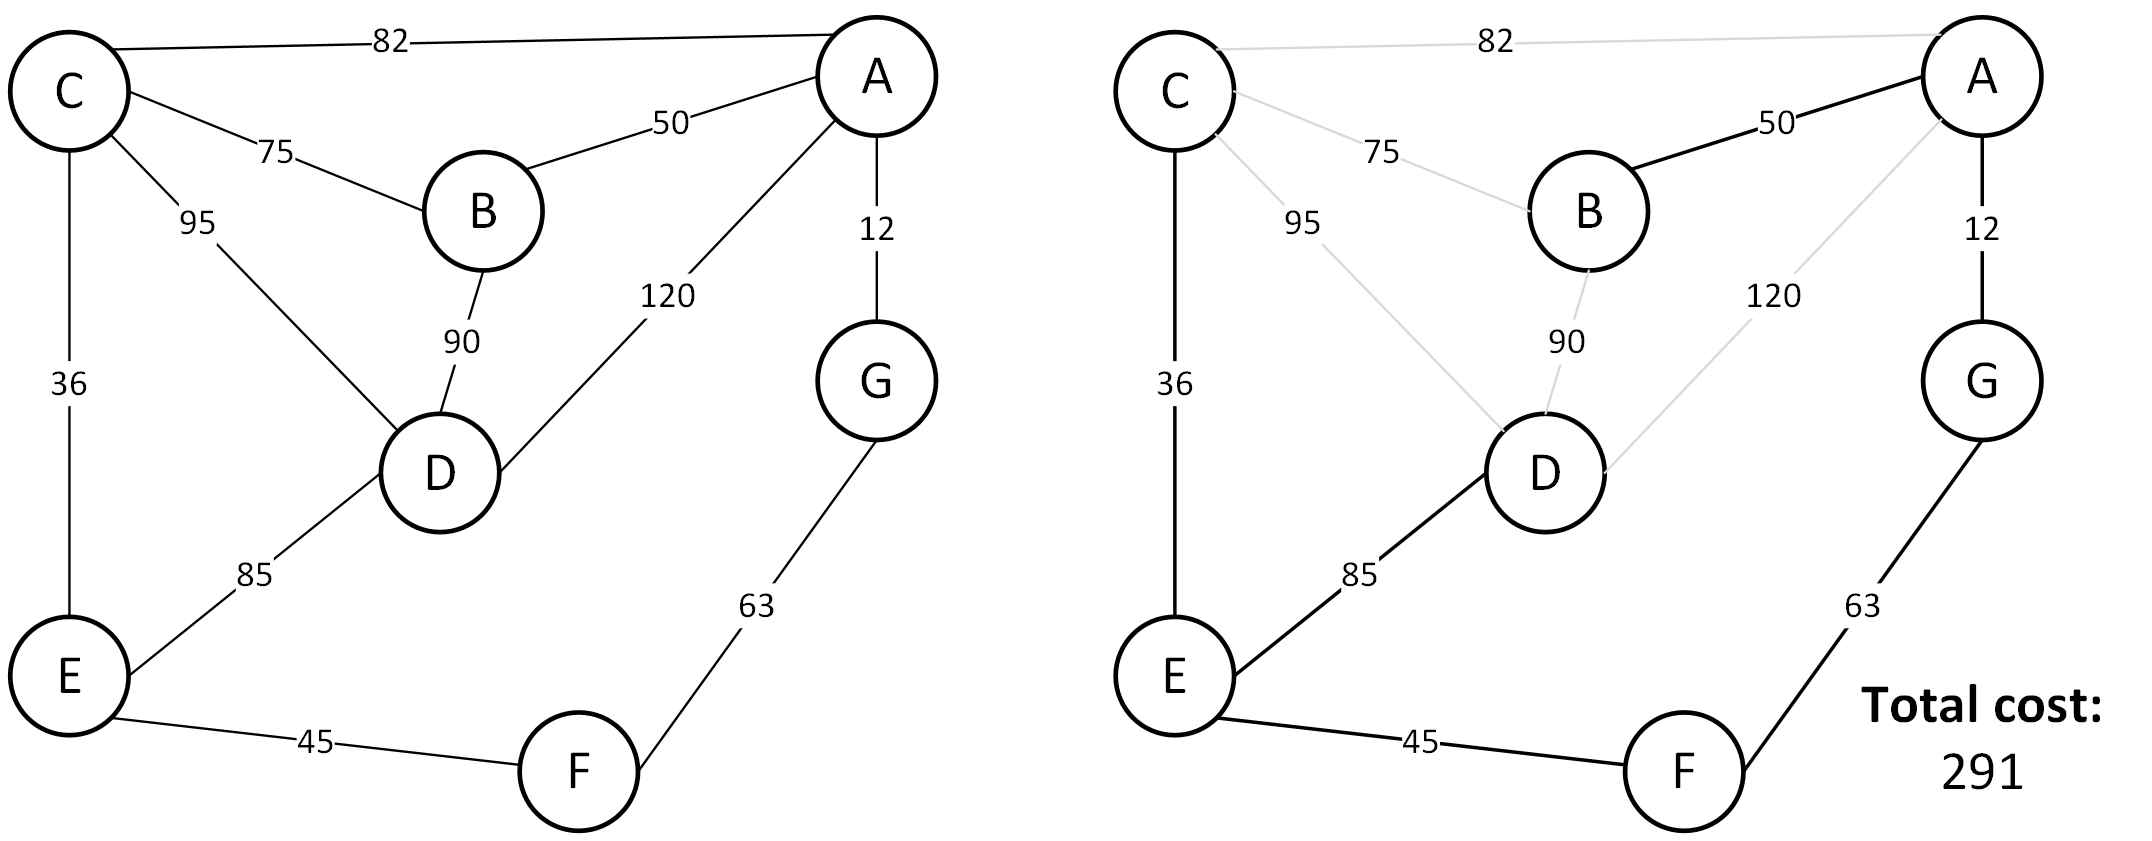
\includegraphics[width=\textwidth]{Minimum-Spanning-Tree}
	\caption{Minimální kostra grafu.}
	\label{fig:minimum-spanning-tree}
\end{figure}

\texttt{GDS} knihovna obsahuje \mbox{Primův} algoritmus. Tento iterativní hladový algoritmus vyžaduje na vstupu specifikovat počáteční vrchol $s$. Postupně je z něj vytvářen strom $T$ tak, že v každém kroku je k $T$ připojena jedna hrana. Vždy je vybrána hrana s nejmenší váhou, která vede z vrcholu v $T$ do vrcholu mimo $T$. Pokud neexistuje hrana, která by šla do stromu přidat, výpočet skončí a vrátí $T$, kde $T$ je minimální kostra komponenty vstupního grafu obsahující $s$. Pokud při implementaci využíváme binární prioritní frontu dostaneme celkovou složitost $O(|E| \log_2 |V|)$.

Tento algoritmus lze využít pro nejlevnější propojení měst vodním potrubím, kde nižší ohodnocení hran znamená menší náklady. Hledání minimální kostry se též využívá při aproximování složitých problémů, jako je například problém obchodního cestujícího.\cite{graphAlgorithms}

\subsection{Random walk}
Při psaní této podkapitoly jsem čerpal převážně ze zdroje \cite{neo4jDoc}. Random walk provádí náhodné sledy zadané délky z daného vrcholu. Jedná se o průchod grafem, kde je vždy v aktuálním vrcholu náhodně vybrána hrana, kterou bude algoritmus pokračovat. V klasické verzi algoritmu je v každém vrcholu pravděpodobnost vybrání hrany uniformní a nezáleží na předchozích výběrech. \texttt{GDS} nabízí sofistikovanější verzi označovanou jako \textit{Random walk druhého řádu}. U tohoto algoritmu se specifikují dva parametry:

\begin{itemize}
\item \texttt{returnFactor} -- určuje snahu algoritmu se vracet zpět do vrcholu, který byl navštíven naposledy. Hodnoty menší než 1 pravděpodobnost tohoto výběru zvyšují.
\item \texttt{inOutFactor} -- určuje snahu algoritmu zůstávat či nezůstávat v blízkosti počátečního vrcholu. Čím vyšší hodnota je zadána, tím bude průchod grafem lokálnější.
\end{itemize}
V klasické verzi jsou oba parametry nastaveny na hodnotu 1. Výběry hran lze též ovlivnit ohodnocením hran.

Random walk se používá jako součást jiných algoritmů, kde je potřeba určité množství náhodných, ale navzájem propojených vrcholů. Může být též využíván pro simulaci šíření epidemie. V následující ukázce byl algoritmus použit na graf s logickým datovým modelem z obrázku \ref{fig:RailNetwork-Graph} z předchozí kapitoly. Algoritmus začínal ve stanici s vlastností \texttt{stationId} rovné 9. Tabulka \ref{tab:randomWalk} ukazuje výsledky algoritmu. Pro jedno nastavení parametrů jsou ukázány tři náhodné cesty o délce sedmi hran. Každá cesta je reprezentována ve druhém sloupci posloupností identifikátorů stanic \texttt{stationId}, přes které cesta prochází. Tyto identifikátory jsou od sebe odděleny středníky. V třetím sloupci je pro každou cestu spočítána vzdálenost vzdušnou čarou z počátečního do cílového vrcholu naznačující, jak lokální průchod algoritmus provedl.

\begin{table}[h]
\caption[Random walk]{Příklady běhu algoritmu random walk.}
\label{tab:randomWalk}
\begin{tabularx}{\textwidth}{ | X | l | l | }
 \hline
 \textbf{Parametry} & \textbf{Vrcholy na cestě} & \textbf{Vzdálenost} \\
 \hline \hline
 \multirow{3}{*}{\shortstack{returnFactor = 20;\\inOutFactor = 0,2;}} & 9; 132; 187; 541; 814; 142; 732; 644 & 29\,596 m \\
 & 9; 686; 1134; 1270; 326; 1061; 523; 19 & 38\,943 m \\
 & 9; 1238; 553; 1174; 368; 648; 916; 1260 & 19\,693 m \\
 \hline
 \multirow{3}{*}{\shortstack{returnFactor = 0,2;\\inOutFactor = 20;}} & 9; 132; 9; 132; 9; 132; 686; 132 & 8\,181 m \\
 & 9; 686; 9; 686; 9; 686; 9; 686 & 9\,587 m \\
 & 9; 686; 9; 686; 132; 9; 132; 9 & 0 m \\
 \hline
\end{tabularx}
\end{table}

\subsection{Algoritmy pro míru centrality}
Při psaní této podkapitoly jsem čerpal převážně ze zdrojů \cite{inAction} a \cite{graphAlgorithms}. V rámci analýzy grafů mohou algoritmy centrality poskytnout vhled do významnosti jednotlivých vrcholů v grafu. Tyto algoritmy umožňují identifikovat vrcholy, které jsou v kontextu celého grafu významnější než ostatní. V praxi je možné využít těchto algoritmů například při analýze kritických sekcí v telekomunikačních nebo počítačových sítích, které slouží jako hlavní přenosové trasy pro informace. Dále lze centrality využít k identifikaci klíčových osobností v rámci organizace či k~detekci odlehlých dat, která mohou naznačovat nekalé praktiky či podvody.

\subsubsection{Degree Centrality}
Nejznámnější a nejjednodušší mírou centrality je degree centrality. Tato míra každému vrcholu v grafu přiřazuje skóre rovné jeho stupni. Stupeň vrcholu může být buď vstupní, výstupní, nebo kombinovaný. Vrcholy s vyšším stupněm lze obecně považovat za důležitější, neboť přes ně může proudit více informací díky většímu počtu hran. Příkladem může být graf reprezentující železniční síť. Čím více spojení má železniční stanice, tím spíše se jedná o významější stanici.

\subsubsection{Closeness Centrality}
Myšlenkou closeness centrality je identifikovat nejvlivnější vrchol v grafu na základě toho, jak rychle je možné se z něj lze dostat do ostatních vrcholů. Konkrétně je to vrchol, pro který je součet nejkratších cest do všech ostatních vrcholů co nejmenší. V případě nesouvislého grafu lze využít \textit{harmonic centrality}, která se umí vypořádat s nedosažitelnými vrcholy. Skóre vrcholu $ u \in V $ v grafu $G = \langle V,E\rangle$ se pak počítá podle vzorce
\begin{equation*}
closenessCentrality(u) = \frac{1}{ \sum_{ v \in V \smallsetminus \{ u \} }{ dist(u,v) } }.
\end{equation*}

\subsubsection{Betweenness Centrality}
Algoritmus pro výpočet betweenness centrality\cite{betweenness-original} nejprve spočítá nejkratší cesty mezi všemi páry různých vrcholů v grafu. Každý vrchol poté obdrží skóre, které je tím vyšší, čím více nejkratších cest vede přes daný vrchol. Tyto hodnoty mohou být klíčové například v grafu, kde vrcholy reprezentují křižovatky a hrany představují cesty mezi nimi. Informace o tom, kterými křižovatkami prochází nejvíce nejkratších cest, můžeme využít pro odhad lokací, kde se pravděpodobně bude pohybovat nejvíce lidí. Základní vzorec pro počítání skóre vrcholu $ u \in V $ v grafu $G = \langle V,E\rangle$ je
\begin{equation*}
betweennessCentrality(u) = \sum_{ v \neq u \neq w \in V } \frac{\delta(u)}{ { dist(v,w) } },
\end{equation*}
kde $\delta(u)$ značí počet nejkratších cest, které prochází vrcholem $u$.

Algoritmy pro closeness a betweenness centrality mohou být v případě velkých grafů výpočetně dost náročné. Proto se často přistupuje k jiným, ne zcela přesným, zato mnohem rychlejším, algoritmům.

\subsubsection{PageRank}
S tímto iterativním algoritmem\cite{pagerank-original} přišla na trh společnost Google. Byl určen pro hodnocení významnosti webových stránek, kde webové stránky si lze představit jako vrcholy grafu. Hrany mezi nimi reprezentují odkazy na stránkách odkazující na jiné stránky. Důležitost vrcholu je určena nejen důležitostí vrcholu samotného, ale také důležitostí vrcholů na tuto stránku odkazujících. Vysoké skóre vrcholu tedy znamená, že je vrchol propojen s vrcholy, které mají též vysoké skóre.

Toto řešení je založeno na vlastních vektorech a stochastických maticích z~lineární algebry. Výpočet skóre většinou vede na nekonečný výpočet a proto se omezuje počet iterací tohoto výpočtu, nebo se udává maximální možná odchylka mezi výsledky iterací.

\subsubsection{Použití algoritmů pro míru centrality}
Výsledky aplikace zmíněných algoritmů pro měření centrality na graf z obrázku \ref{fig:example-graph} je znázorněn v tabulce \ref{tab:centralityResults}.

\begin{figure}[h]
	\centering
	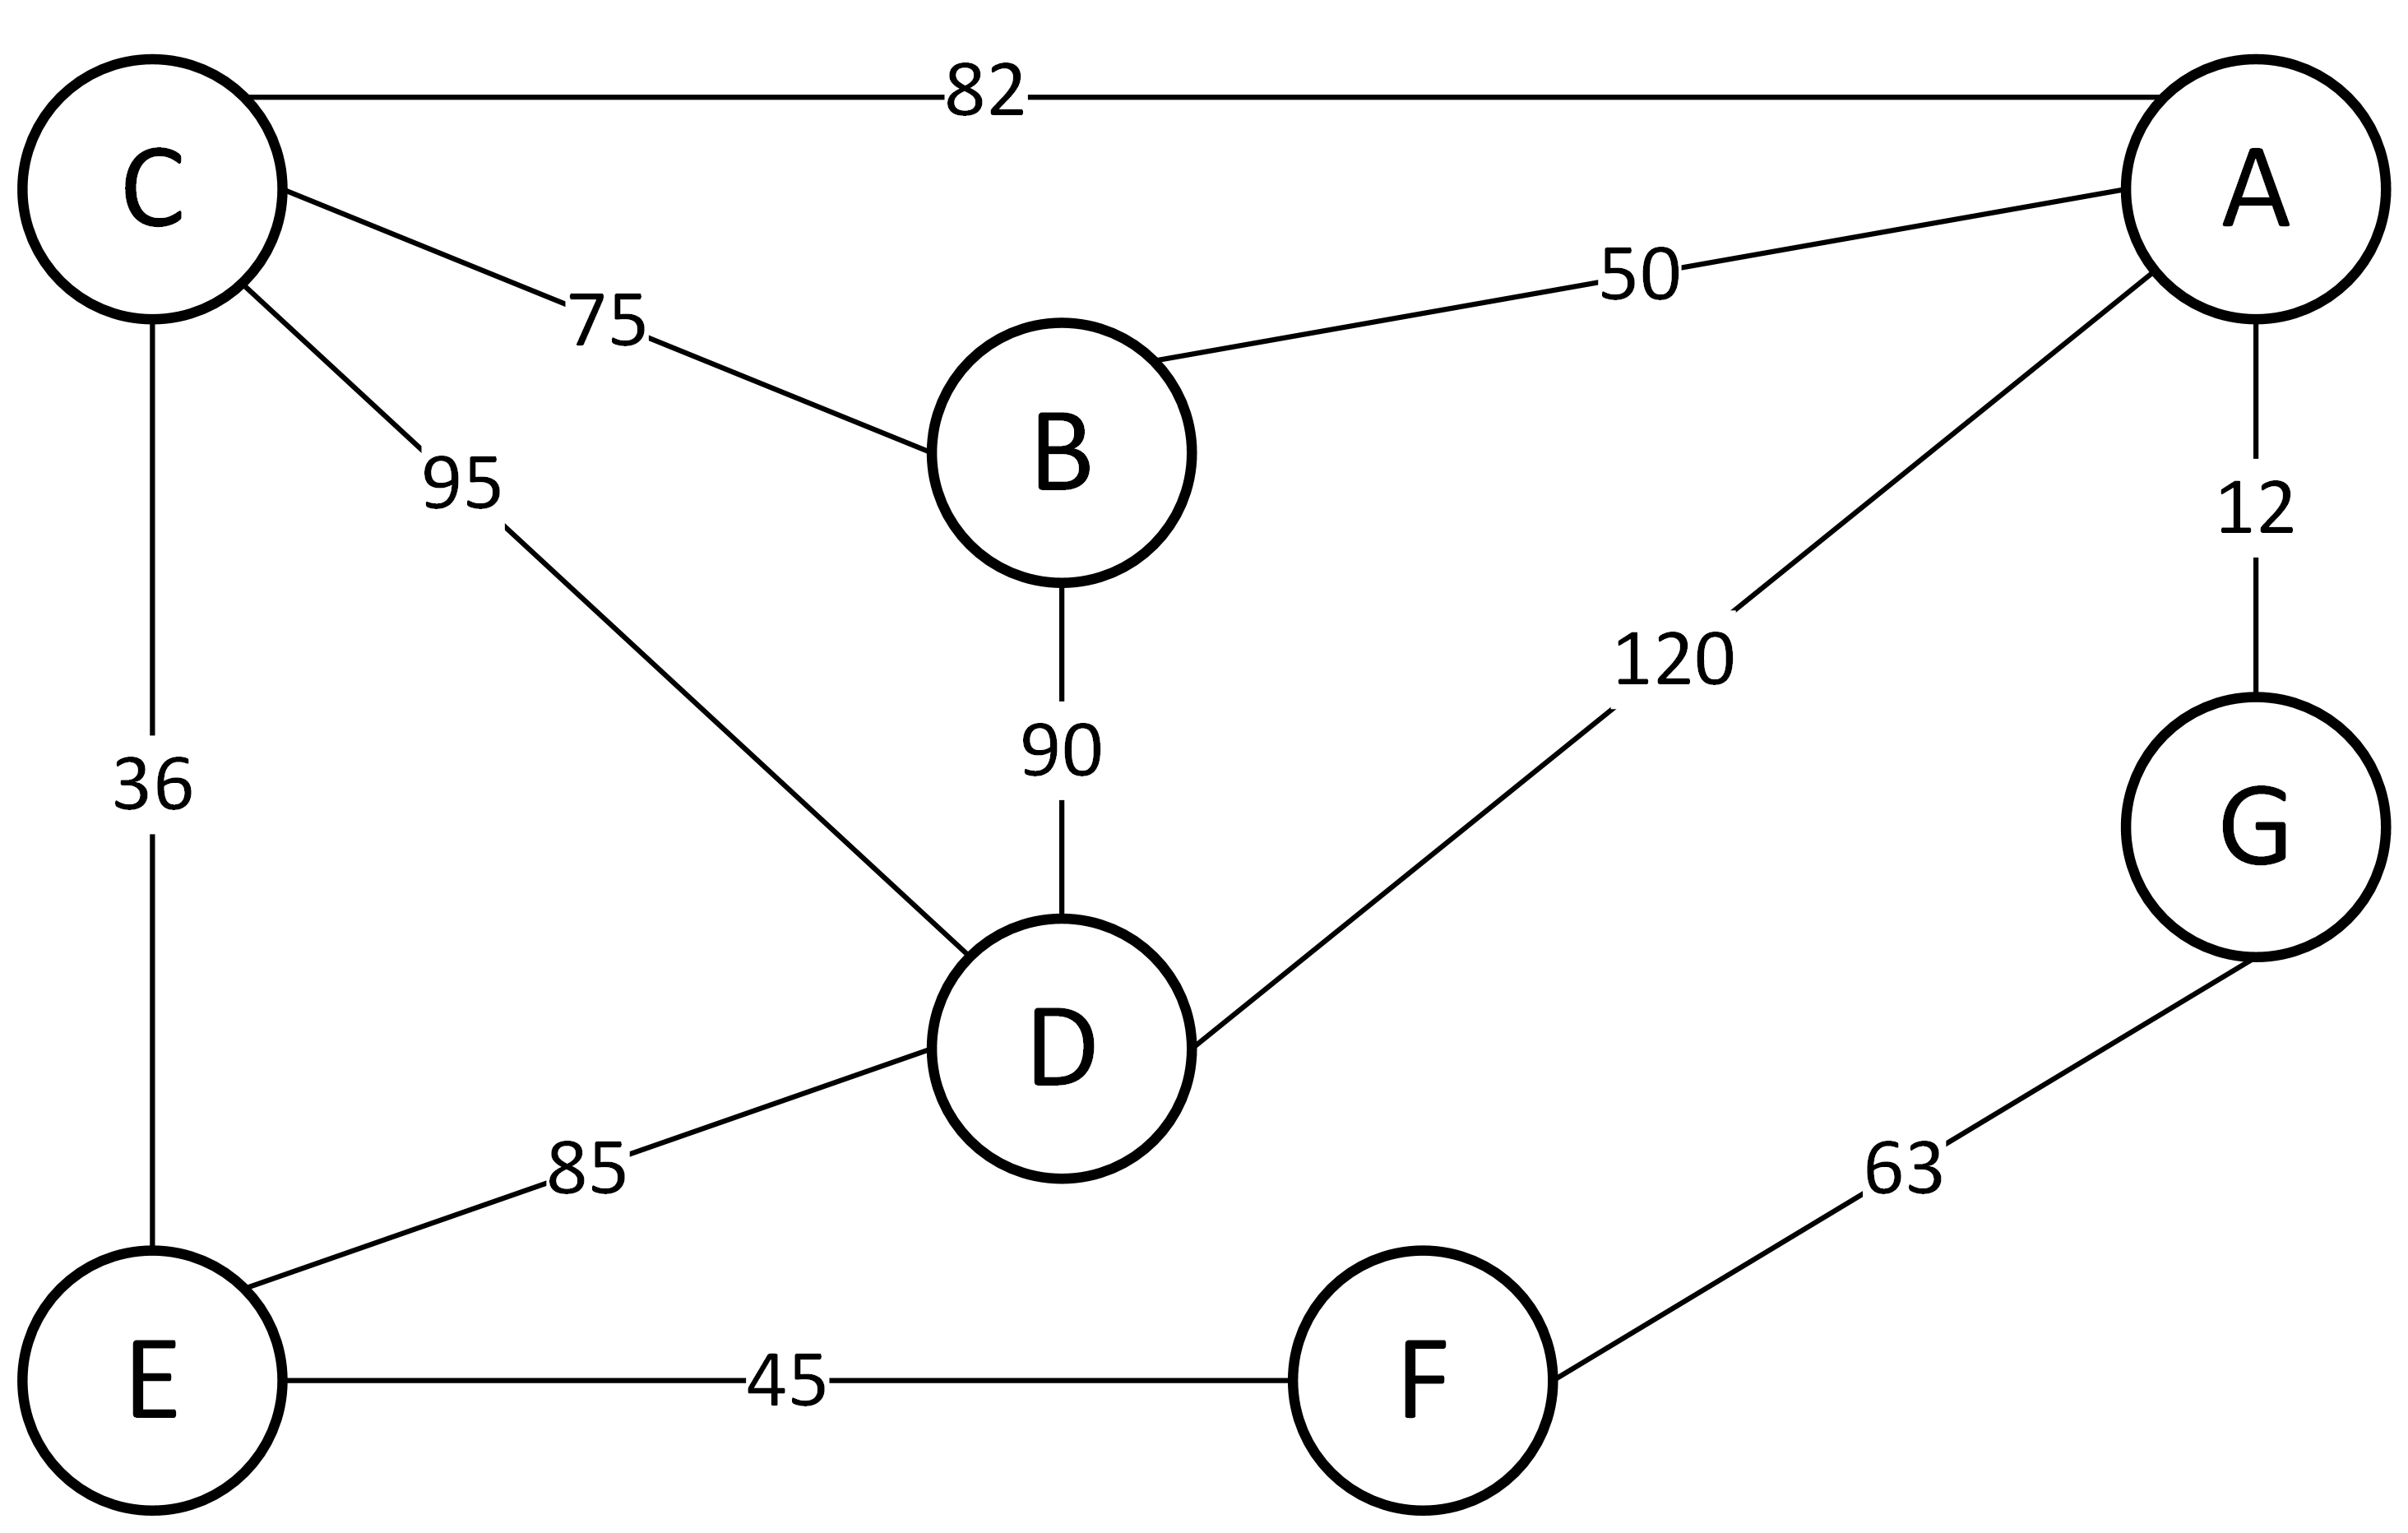
\includegraphics[scale=0.3]{ExampleGraph}
	\caption[Graf pro ukázkové příklady.]{Příklad grafu, na kterém jsou prováděny algoritmy.}
	\label{fig:example-graph}
\end{figure}

\begin{table}[h]
\begin{center}
\caption{Míry centrality.}
\label{tab:centralityResults}
\begin{tabular}{ | l || c | c | c | c | c | c | c | }
 \hline
 \textbf{Vrchol} & A & B & C & D & E & F & G \\
 \hline
 \textbf{Degree Centrality} & 4 & 3 & 4 & 4 & 3 & 2 & 2 \\
 \hline
 \textbf{Closeness Centrality} & 0,75 & 0,6 & 0,75 & 0,75 & 0,67 & 0,55 & 0,6 \\
 \hline
 \textbf{Betweeness Centrality} & 3,33 & 0 & 1,33 & 1,33 & 2,67 & 1 & 1,33 \\
 \hline
\end{tabular}
\end{center}
\end{table}

\subsection{Detekce komunit}
Při psaní této podkapitoly jsem čerpal převážně ze zdrojů \cite{graphAlgorithms} a \cite{neo4jDoc}. Algoritmy detekce komunit v grafech se zaměřují na nalezení skupin vrcholů, tzv. \textit{komunit}, které jsou mezi sebou silněji propojeny než s vrcholy v jiných částech grafu. Příkladem využití je analýza sociálních sítí, kde se hledají komunity blízkých přátel, které tvoří shluky propojených vrcholů. Následně lze z těchto informací odhadovat chování jednotlivců podle členů jejich komunity. Znalost komunit lze též využít pro doporučování produktů uživatelům s podobným nákupním chováním.

Algoritmy pro detekci komunit se dělí na \textit{deterministické} a \textit{nedeterministické}. Deterministické vrací pro stejný graf vždy stejný výsledek, zatímco výsledek u nedeterministických může být pro stejný graf při opakovaném spuštění mírně odlišný. Mezi deterministické se řadí počítání trojúhelníků, výpočet shlukavacího koeficientu, nebo hledání komponent. Mezi nedeterministické patří například Label Propagation, nebo Louvain Modularity.

\subsubsection{Počítání trojúhelníků a shlukovacího koeficientu}
Algoritmus pro každý vrchol vrátí počet \textit{trojúhelníků}, kterých je daný vrchol součástí. Trojúhelník je zde definován jako skupina tří navzájem propojených vrcholů. Trojúhelníky nám pomáhají určit do jaké míry jsou vrcholy v našem grafu propojeny. V hustých grafech, lze obvykle nalézt více trojúhelníků. Algoritmus je oblíbený při analýze sociálních sítí, kde pomáhá detekovat komunity, nebo zkoumání skupin webových stránek s podobným námětem podle odkazů mezi nimi.

Znalost počtu trojúhelníků lze využít též pro výpočet \textit{shlukovacího koeficientu} vrcholu, který určuje pravděpodobnost, s jakou jsou jeho sousedé propojeni -- tvoří s ním trojúhelník. Pokud je hodnota koeficientu rovna 1, znamená to, že vrchol se svými sousedy tvoří kliku v grafu. Shlukovací koeficient vrcholu $u$ lze vypočítat pomocí vzorce

\begin{equation} 
\label{eq:ClusteringCoefficient}
ClusteringCoefficient(u) = \frac{2 * TriangleCount(u)}{deg(u) * (deg(u) - 1)}.
\end{equation}

Pro ukázkový graf na obrázku \ref{fig:example-graph} počet trojúhelníků a shlukovací koeficient jednotlivých vrcholů zobrazuje tabulka \ref{tab:triangles}. Vidíme, že vrchol A je součástí tří trojúhelníků, které jsou tvořeny vrcholy A-B-C, A-B-D a A-C-D. Stupeň vrcholu je 4. Dosazením do vzorce \ref{eq:ClusteringCoefficient} dostáváme shlukovací koeficient 0.5.

\begin{table}[h]
\begin{center}
\caption{Počet trojúhelníků a shlukovací koeficient.}
\label{tab:triangles}
\begin{tabular}{ | l || c | c | c | c | c | c | c | }
 \hline
 \textbf{Vrchol} & A & B & C & D & E & F & G \\
 \hline
 \textbf{Triangle Count} & 3 & 3 & 4 & 4 & 1 & 0 & 0 \\
 \hline
 \textbf{Clustering Coefficient} & 0,5 & 1 & 0,67 & 0,67 & 0,33 & 0 & 0 \\
 \hline
\end{tabular}
\end{center}
\end{table}

\subsubsection{Hledání komponent}
Nalezení komponent v grafu je užitečné pro pochopení našich dat. Algoritmy pro tuto úlohu jsou rychlé. Mohou být využívány v grafech, které se často aktualizují pro detekci nových vrcholů mezi skupinami. Nebo jsou použity pro hrubé nalezení komunit, které lze dál analyzovat.  Existují algoritmy pro hledání silně a~slabě souvislých komponent. Pro graf na obrázku \ref{fig:example-graph} nám algoritmus pro hledání slabě souvislých komponent vrátí, že všechny vrcholy grafu jsou součástí jedné komponenty.

\subsubsection{Algoritmus Louvain}
Louvainův algoritmus\cite{louvain-original} je hladový a iterativní algoritmus, který se snaží maximalizovat modularitu komunit. Mudularita je způsob, jakým můžeme měřit kvalitu nalezených komunit. Porovnává komunity v grafu s náhodným grafem, který vznikne odstraněním hran v původním grafu a následným přidáním těchto hran mezi dva náhodně zvolené nepropojené vrcholy. U náhodného grafu se předpokládá rovnoměrné propojení těchto vrcholů. Modularita nabývá hodnot z intervalu $\langle -1, 1\rangle$. Čím je hodnota vyšší, tím jsou vrcholy v komunitách propojenější. Výpočet modularity je počítán vzorcem
\begin{equation} 
\label{eq:louvain}
M = \frac{1}{2m} \sum_{u,v} [A_{uv} - \frac{k_u k_v}{2m}] \delta (C_u, C_v),
\end{equation}
kde
\begin{itemize}
\item $u$ a $v$ jsou vrcholy,
\item $m$ je součet přes všechna ohodnocení hran,
\item $A_{uv}$ je váha hrany mezi vrcholy $u$ a $v$,
\item $k_x$ je součet přes všechna ohodnocení hran incidentních s $x$
\item a 
$
 \delta (C_u, C_v)=
    \begin{cases}
        1 & \text{jestliže } u \text{ i } v \text{ patří do stejné komunity,} \\
        0 & \text{jinak.}
    \end{cases}
$
\end{itemize}
Podíl $\frac{k_u k_v}{2m}$ ve vzorci \ref{eq:louvain} odpovídá náhodnému grafu mající stejnou distribuci stupňů a tedy vyjadřuje očekávanou sumu ohodnocení hran mezi dvěma vrcholy.

Na začátku každý vrchol tvoří komunitu. V neohodnoceném grafu má každá hrana váhu 1. Algoritmus má dva kroky:
\begin{enumerate}
\item Pro každý vrchol (komunitu) $v$ v grafu je vyhodnocována změna modularity, pokud by se vrchol přemístil do jedné ze sousedních komunit. Vyhodnocuje se pomocí vzorce \ref{eq:louvain}. Jestliže je hodnota modularity pro všechny sousedy záporná, pak vrchol $v$ zůstane ve vlastní komunitě. Jinak je vrchol $v$ sloučen do komunity, pro kterou je hodnota modularity nejvyšší. Cílem je najít nejlepší rozřazení jednotlivých vrcholů do komunit.
\item Každá nalezená komunita tvoří vrchol v novém grafu. Každému vrcholu je vytvořena smyčka s váhou rovnou součtu ohodnocení hran v rámci komunity. Hrana propojující dva nově vzniklé vrcholy má váhu, která je součtem ohodnocení hran mezi komunitami, které tyto vrcholy reprezentují. Tento nový graf bude vstupem v další iteraci.
\end{enumerate}
Algoritmus iteruje tak dlouho, dokud dochází ke zvyšování modularity ve vzniklých komunitách. Dá se též omezit, aby iteroval tak dlouho, dokud budou hodnoty modularity vyšší než zadaná prahová hodnota. Výsledkem je rozřazení vrcholů do jednotlivých komunit na~základě výsledného grafu.\cite{louvain}

Pro ukázkový graf \ref{fig:example-graph} nám algoritmus z knihovny \texttt{GDS} rozdělil vrcholy do~dvou komunit. Výsledky shrnuje tabulka \ref{tab:louvain}.

\begin{table}[h]
\begin{center}
\caption{Algoritmus Louvain.}
\label{tab:louvain}
\begin{tabular}{ | l || c | c | c | c | c | c | c | }
 \hline
 \textbf{Vrchol} & A & B & C & D & E & F & G \\
 \hline
 \textbf{Komunita} & 2 & 2 & 2 & 2 & 6 & 6 & 6 \\
 \hline
\end{tabular}
\end{center}
\end{table}
\clearpage
\section{Testování vybraných implementací}
Pro testování byl použit dataset \cite{youtubeDataset} obsahující informace o vztazích uživatelů ze sociální sítě Youtube. Pro testování byl též vytvořen csv soubor obsahující identifikátory všech uživatelů v síti a další soubor s vlastnostmi. Tato data tvoří neorientovaný graf. Při testování byly použity orientované hrany a obecně byly procházeny jak výchozí, tak příchozí hrany. Příslušný logický datový model k testovanému datasetu ukazuje obrázek \ref{fig:Youtube-Graph}. Seznam souborů shrnuje tabulka \ref{tab:Youtube-csv}.

\begin{figure}[h]
\begin{center}
	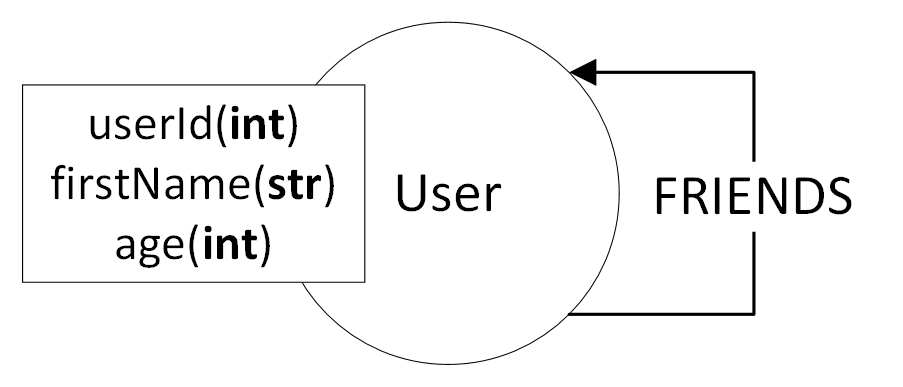
\includegraphics[scale=0.75]{Youtube-Graph}
	\caption[Grafový model pro testování.]{Logický grafový model pro testování.}
	\label{fig:Youtube-Graph}
\end{center}
\end{figure}

\begin{table}[h]
\caption{Použité soubory pro experimentování s databázemi.}
\label{tab:Youtube-csv}
\begin{tabularx}{\textwidth}{ | l | c | c | X | }
 \hline
 \textbf{Typ} & \textbf{Název souboru} & \textbf{Počet} & \textbf{Informace o souboru} \\
 \hline \hline
 Entity & \texttt{users.csv} & 1\,134\,890 & Identifikátory uživatelů. \\
 \hline
 Vztahy & \texttt{com-youtube.ungraph.tsv} & 2\,987\,624 & Přátelství mezi uživateli.\\
 \hline
 Vlastnosti & \texttt{properties.csv} & 1\,134\,890 & Jméno a věk uživatelů.\\
 \hline
\end{tabularx}
\end{table}

Průměrný stupeň vrcholu je 5,265. Medián a modus jsou 1. První kvartil je roven 1 a třetí kvartil je roven 3. Největší stupeň ze všech vrcholů má vrchol s identifikátorem 1\,072, který má stupeň 28\,754. Částečnou distribuci stupně vrcholů zobrazuje graf \ref{fig:youtube-log}. Pro zvýšení přehlednosti bylo na vertikální ose použito logaritmické měřítko o základu 10. Horizontální osa zobrazující stupně vrcholů byla omezena na interval $\langle 0,2000\rangle$.

\begin{figure}[h]
	\centering
	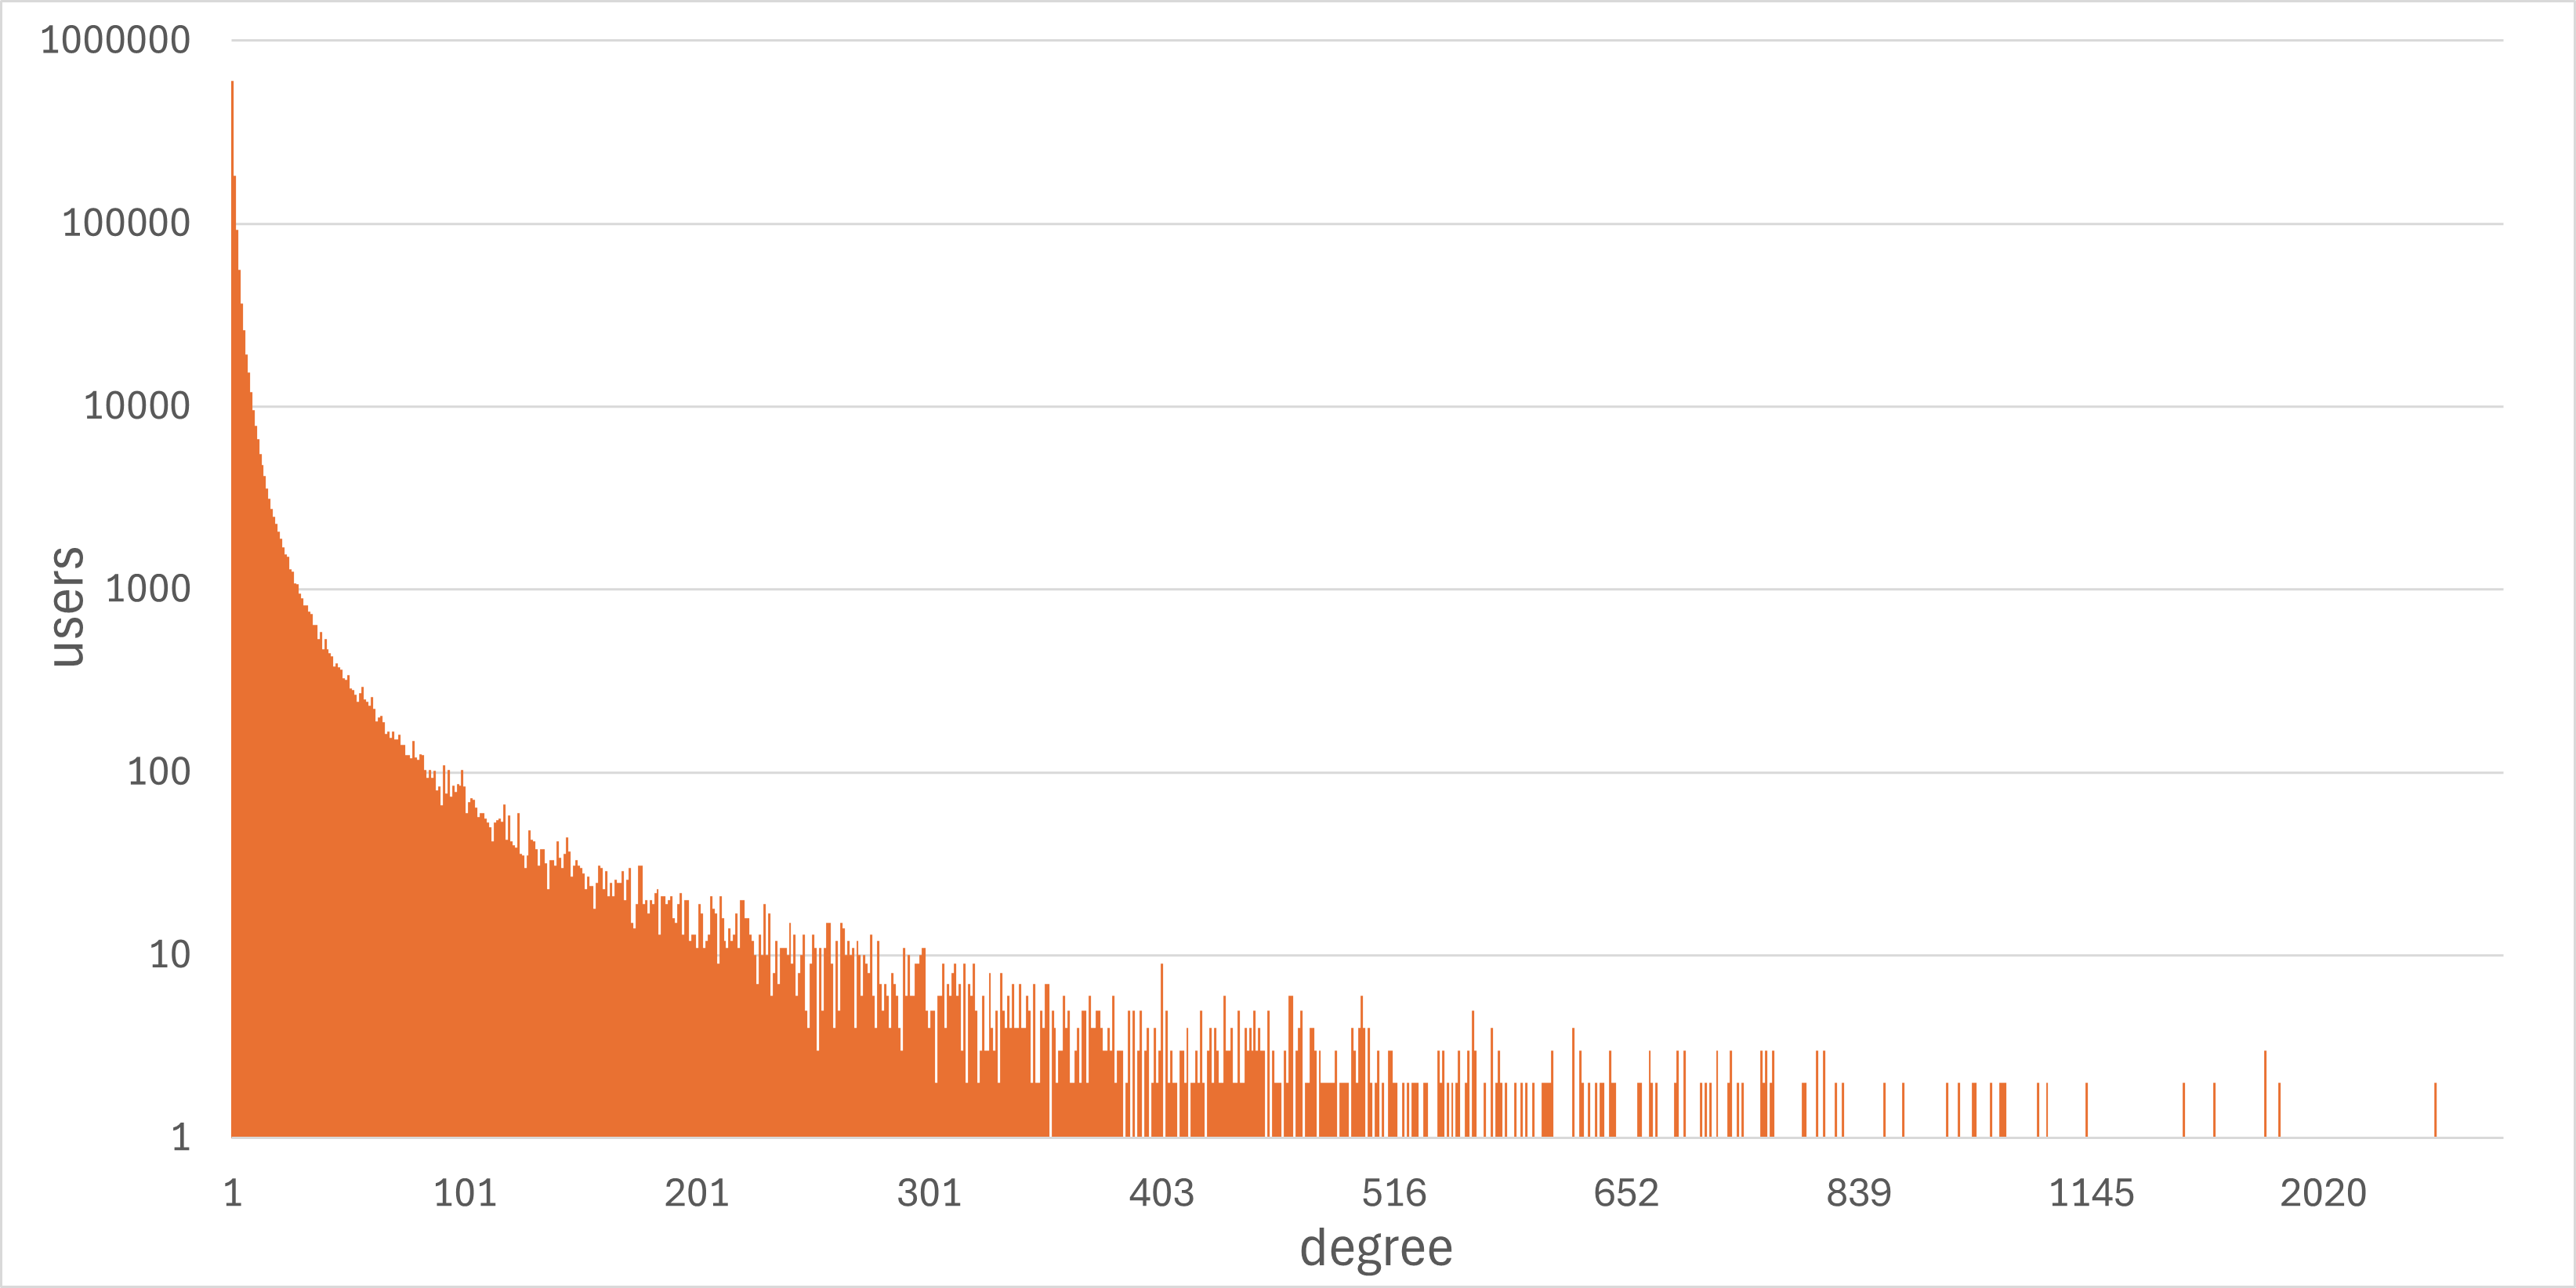
\includegraphics[width=\textwidth]{youtube-log}
	\renewcommand{\figurename}{Graf}
	\caption[Distribuce stupně vrcholů]{Distribuce stupně vrcholů testovaného datasetu.}
	\label{fig:youtube-log}
\end{figure}

Testování probíhalo na notebooku s operační pamětí o velikosti 16 GB. Notebook byl po celou dobu testování napájen. Konfiguraci databází jsem ponechal v původním stavu, neboť tak podávaly nejlepší výsledky. Pouze jsem upravil velikost Java Heap v Gremlin konzoli na 4 GB. V Gremlin konzoli jsem pracoval s lokální databází pomocí módu \texttt{plocal}, protože výsledky byly mnohonásobně lepší. U testování výkonu procházení grafu a hledání nejkratší cesty jsem provedl první pokus, abych viděl, jak funguje cache. Následně byl každý dotaz proveden desetkrát. Z těchto výsledků pak byla vypočítána průměrná doba dotazu.

Pro snazší zprovoznění zvolených databázových systémů jsem pro každou databázi vytvořil složku obsahující soubor \texttt{Dockerfile}, což umožňuje snadné spuštění databázového systému v Docker kontejneru. Do těchto kontejnerů jsou zkopírovány všechny používané datasety a potřebné soubory. Ke každé databázi jsou též k dispozici okomentované dotazy. Testy v Dockeru mi podávaly mírně horší výsledky než výsledky prezentované v této práci, které byly prováděny na~lokálně stažených databázových systémech.

\subsection{Výsledky testování}

První jsem testoval vkládání a mazání vrcholů a hran v databázích. Data do~databáze Neo4j byla vložena pomocí klauzule \texttt{LOAD CSV} v transakcích. Pro vložení dat do databáze ArangoDB byl použit nástroj \texttt{arangoimport}. Pro databázi OrientDB byl použit nástroj \texttt{ETL}. Mazání vrcholů a hran probíhalo pomocí dotazovacího jazyka dané databáze. V OrientDB jsem mazal vrcholy pouze pomocí SQL. Výsledky testu zobrazuje graf \ref{fig:insertDelete}.

\begin{figure}[h]
	\centering
	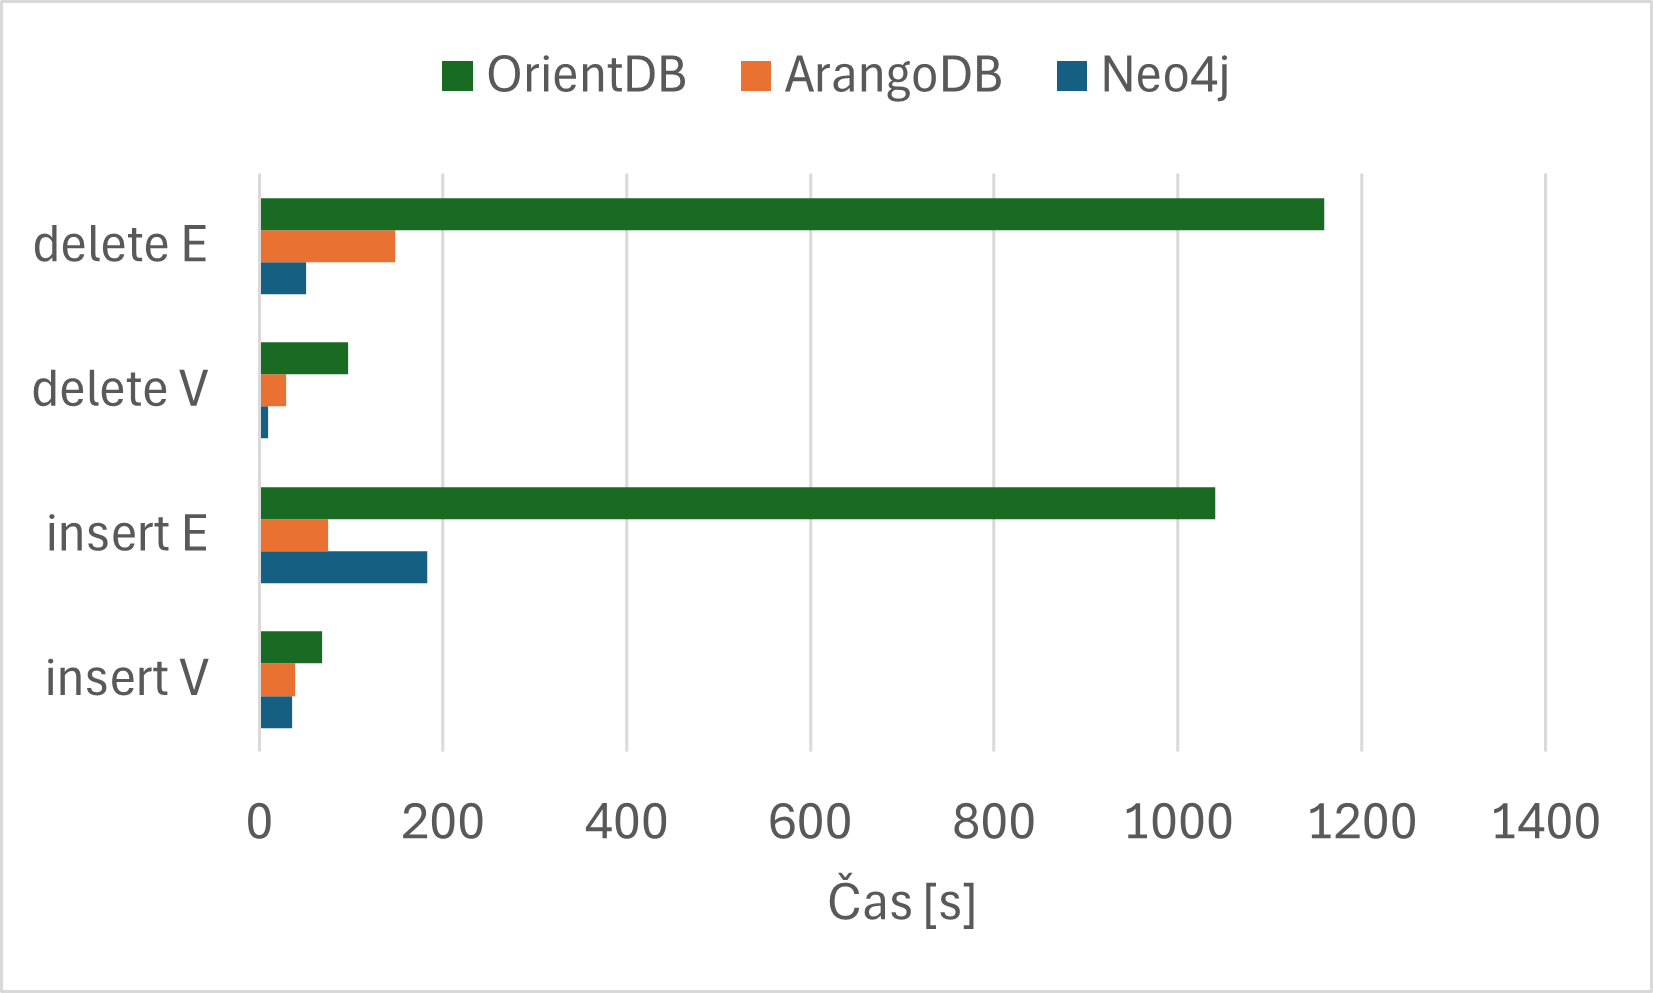
\includegraphics[width=\textwidth]{insertDelete}
	\renewcommand{\figurename}{Graf}
	\caption{Průměrné výsledky dotazů vkládání a mazání.}
	\label{fig:insertDelete}
\end{figure}

Následně jsem otestoval výkon databází pomocí osmi dotazů. Inspiroval jsem se dotazy používanými ve zdroji \cite{benchmark}. První čtyři dotazy testují průchod grafem. Další dva hledají nejkratší cestu. Pro poslední dva dotazy jsem do databáze přidal pomocí výše zmíněných importovacích nástrojů vlastnosti ze souboru \texttt{properties.csv}. Sloužily k otestování filtrování a agregování. Na tyto vlastnosti nebyl použitý index. Ten jsem použil pouze pro vlastnost \texttt{userId}. Všechny dotazy jsou shrnuty v tabulce \ref{tab:test-queries}. Grafy \ref{fig:queryResults} a \ref{fig:queryResults2} ukazují průměrnou dobu trvání jednotlivých dotazů.

\begin{table}[h]
\caption[Použité dotazy pro testování]{Tabulka použitých dotazů při testování databází.}
\label{tab:test-queries}
\begin{tabularx}{\textwidth}{ | l | X | l | }
 \hline
 \textbf{Dotaz} & \textbf{Popis dotazu} & \textbf{Výsledek} \\
 \hline \hline
 Q1 & Spočítá sousedy vrcholu s userId 1 do hloubky 2. & 7\,176 \\
 \hline
 Q2 & Spočítá sousedy vrcholu s userId 1 do hloubky 3. & 240\,249\\
 \hline
 Q3 & Spočítá sousedy vrcholu s userId 1 do hloubky 4. & 814\,122 \\
 \hline
 Q4 & Spočítá sousedy vrcholu s userId 1 do hloubky 5. & 1\,051\,030\\
 \hline
 Q5 & Najde nejkratší neorientovanou cestu mezi dvěma vrcholy s userId 12000 a 1047. & 3 hrany \\
 \hline
 Q6 & Hledá nejkratší orientovanou cestu z vrcholu s userId 12000 do vrcholu s userId 1047, přičemž cesta neexistuje. & null \\
 \hline
 Q7 & Vrátí počet uživatel starších 75 let, jejichž jméno začíná na řetězec \uv{Ma}. & 13\,779 \\
 \hline
 Q8 & Vrátí průměrný věk uživatelů jmenujících se \uv{James}. & 56,574 let\\
 \hline
\end{tabularx}
\end{table}

\begin{figure}
\centering
 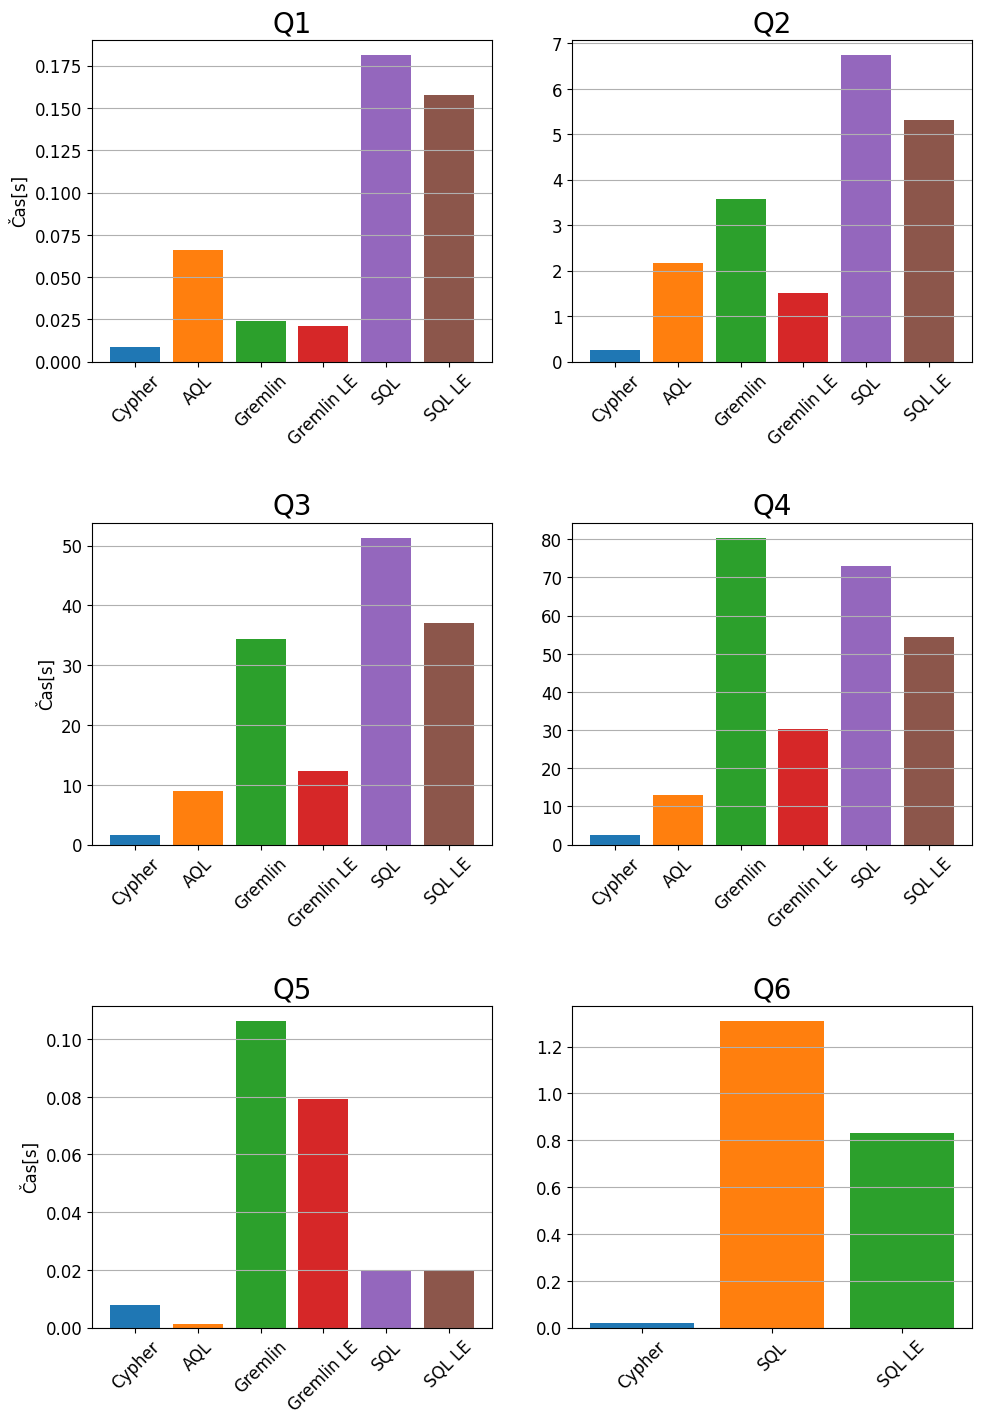
\includegraphics[width=\textwidth]{results}
\renewcommand{\figurename}{Graf}
\caption{Průměrné výsledky dotazů Q1-Q6.}
\label{fig:queryResults}
\end{figure}

\begin{figure}
\centering
 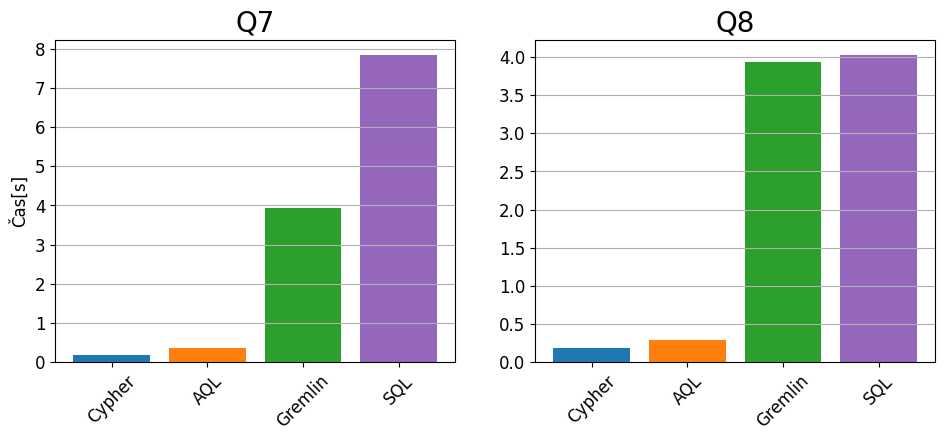
\includegraphics[width=\textwidth]{properties-test}
\renewcommand{\figurename}{Graf}
\caption{Průměrné výsledky dotazů Q7 a Q8.}
\label{fig:queryResults2}
\end{figure}

\subsection{Shrnutí}
Následuje shrnutí výsledků výkonostních testů jednotlivých databází. To jsem rozdělil na tři podkapitoly, kde se v každé věnuji jedné databázi.

\subsubsection{OrientDB}
Při vkládání a mazání byly mnou naměřené výsledky i více než 14krát horší než u dalších databází. Přitom bylo dodrženo doporučení z dokumentace -- hodnota WAL nastavena na hodnotu \texttt{false}. Mnou naměřené výsledky databází OrientDB a Neo4j víceméně odpovídají výsledkům experimentu \cite{experimentalComparision}.

Pro porovnání výkonu zpracování dotazů Q1-Q8 jsem dotazy zadával jak v~jazyce SQL pro OrientDB databázi, tak v~jazyce Gremlin. Pro zlepšení výsledků jsem také zkusil dotazy Q1-Q6 spustit v databázi používající lightweight hrany (dotazy s nimi jsou na grafu \ref{fig:queryResults} označeny jako LE). V případě jazyka Gremlin se pak vyhodnocení dotazů v databázi s lightweight hranami více než dvakrát zrychlilo. Pokud tedy není potřeba uchovávat na hranách vlastnosti, z testování plyne, že je dobré kvůli výkonu i prostoru v úložišti použít lightweight hrany.

Vyhodnocení většiny dotazů bylo v jazyce Gremlin výrazně rychlejší, než v~případě SQL. Dotaz Q5 byl rychlejší v OrientDB SQL pomocí zabudované funkce \texttt{SHORTEST\_PATH}. Pomocí jazyka Gremlin jsem nedostal odpověď na~dotaz Q6 ani po čtyřiceti minutách běhu. Výsledku se dá dočkat, pokud omezíme průchod grafem nastavením limitu pro délku cesty.

V porovnání s ostatními databázemi však OrientDB silně zaostávala. Z výsledků zkoumání \cite{benchmark} jsem očekával, že vyhodnocení dotazů Q3 a Q4 bude v~OrientDB rychlejší než v Neo4j. Mnou naměřené výsledky však byly i více než desetkrát horší.

Dokumentace OrientDB není v porovnání s ostatními příliš přehledná. Setkal jsem se s odkazy na prázdné webové stránky a to i v rámci webového rozhraní OrientDB Studio. Problémy s databází se mi řešily hůře než u ostatních, neboť komunita OrientDB na internetu není tak velká. Při importování dat se někdy do databáze nevložily všechny vrcholy a hrany, i když soubor určený pro import byl stejný. Podle dokumentace stačí v JSON souboru určeném pro konfiguraci importu nastavit hodnotu \texttt{useLightweightEdges} na \texttt{true} pro vložení lightweight hran. Nicméně, i při tomto nastavení se hrany vkládaly jako regulární. Pomohlo až nastavení lightweight hran přes OrientDB Studio.

\subsubsection{ArangoDB}
V prvním testu při vkládání hran byla ArangoDB rychlejší než Neo4j. Jinak se databáze většinou pohybovala mezi dalšími dvěmi testovanými databázemi.  Jediným větším problémem byl dotaz Q6 na hledání nejkratší cesty, mezi dvěma nepropojenými vrcholy. Ani po čtyřiceti minutách se nezastavil, když jsem využil vestavěnou funkci \texttt{SHORTEST\_PATH}.

\subsubsection{Neo4j}
Neo4j byla dle očekávání ve zpracování dotazů nejrychlejší. Při práci s databází jsem nenarazil na žádný problém. Jedním z důvodů jistě bylo zaměření databáze pouze na grafy, oproti multimodelovým konkurentům. Výsledky prvních pokusů pro testování cache se výrazněji nelišily od následujících testů v porovnání s~ostatními testovanými databázemi.

%% Závěry práce. V jazyce práce a anglicky. Text pro jiný než
%% nastavený jazyk práce (nepovinným parametrem language makra
%% \documentclass, výchozí český) se zadává použitím makra s uvedením
%% jazyka jako nepovinného parametru.
\begin{kiconclusions}
Cílem práce bylo představit grafové databáze. Popsal jsem principy ukládání a praci s daty ve formě grafu. V práci jsem se věnoval modelování grafových dat a následně hlavní přednosti grafových databází -- cestování grafem. Představil jsem tři kategorie grafových algoritmů používaných v grafových databázích. Konkrétně to byly algoritmy pro hledání cest, míru centrality a detekci komunit.

V praktické části jsem se věnoval vybraným známým grafovým databázovým systémům a ukázkám jejich použití. Demonstroval jsem na nich jednotlivé problémy zmiňované v textu práce. Následně jsem vybral dataset, na kterém byly vybrané implementace experimentálně porovnány. Nejlepší výsledky při testování podávala databáze Neo4j. Pro jednodušší zprovoznění jsem pro jednotlivé databáze vytvořil \texttt{Dockerfile} s potřebným nastavením.

Práce by se dala rozšířit o porovnání více implementací grafových databází. Toto porovnání by bylo mnohem přínosnější provést za přísnějších podmínek, které by zajistilo mnohem vyšší přesnost testování. Také by mohla být věnována větší pozornost grafovým databázím implementující RDF model nebo hypergraf.

\end{kiconclusions}

\begin{kiconclusions}[english]
The aim of the thesis was to introduce graph databases. I described the principles of storing and working with data in the form of a graph. In the thesis, I focused on graph data modeling and subsequently the main advantages of graph databases -- graph traversal. I introduced three categories of graph algorithms used in graph databases. Specifically, these were algorithms for path finding, centrality measure, and community detection.

In the practical part, I focused on selected well-known implementations of graph databases and examples of their usage. I demonstrated on them the individual problems mentioned in the text of the thesis. Subsequently, I selected a dataset on which the selected implementations were experimentally compared. The best test results were given by database Neo4j. For easier commisioning, I've created a \texttt{Dockerfile} for each database with the necessary configurations.

The thesis could be expanded by comparing more implementations of graph databases. This comparison would be much more beneficial if conducted under stricter conditions to ensure much higher testing accuracy. Also, greater attention could be devoted to graph databases implementing the RDF model or hypergraph.
\end{kiconclusions}


%% -------------------------------------------------------------------

%% Sazba volitelného seznamu zkratek, za přílohami.

%\printglossary

%% Sazba povinné bibliografie, za přílohami (případně i za seznamem
%% zkratek). Při použití BibLaTeXu použijte makro
%% \printbibliography. jinak prostředí thebibliography. Ne obojí!

%% Sazba i v textu necitovaných zdrojů, při použití
%% BibLaTeXu. Volitelné.
%\nocite{*}
%% Vlastní sazba bibliografie při použití BibLaTeXu.
\printbibliography

%% Sazba volitelného rejstříku, za bibliografií.
%\printindex

\end{document}

%%% Local Variables:
%%% mode: latex
%%% TeX-master: t
%%% End:
